\documentclass[12pt, a4paper]{extarticle}


% Russian text support
\usepackage[T2A]{fontenc}
\usepackage[utf8]{inputenc}
\usepackage[russian]{babel}

% Some useful packages
\usepackage{indentfirst}
\usepackage{etoolbox}
\usepackage{amsmath}
\usepackage{amssymb}
\usepackage{amsfonts}
\usepackage{xcolor}
\usepackage{indentfirst}
\usepackage{listings}
\usepackage{mathtools}
\usepackage{tabularx}
\usepackage{caption}
\usepackage{placeins}
\usepackage[bottom]{footmisc}

\captionsetup{skip=0pt}

% Codestyle
\definecolor{codegreen}{rgb}{0,0.6,0}
\definecolor{codegray}{rgb}{0.5,0.5,0.5}
\definecolor{codepurple}{rgb}{0.58,0,0.82}
\definecolor{backcolour}{rgb}{1,1,1}

\lstdefinestyle{mystyle}{
    backgroundcolor=\color{backcolour},   
    commentstyle=\color{codegreen},
    keywordstyle=\color{magenta},
    numberstyle=\tiny\color{codegray},
    stringstyle=\color{codepurple},
    basicstyle=\ttfamily\footnotesize,
    breakatwhitespace=false,         
    breaklines=true,                 
    captionpos=b,                    
    keepspaces=true,                 
    numbers=left,                    
    numbersep=5pt,                  
    showspaces=false,                
    showstringspaces=false,
    showtabs=false,                  
    tabsize=2
}

\lstset{style=mystyle}

\makeatletter
\renewcommand*{\@biblabel}[1]{\hfill #1.}
\makeatother

%
% Remove References header completely
% Stolen from original article.cls
%
\makeatletter
\renewenvironment{thebibliography}[1]{%
%     \section*{\refname}%
%      \@mkboth{\MakeUppercase\refname}{\MakeUppercase\refname}%
      \list{\@biblabel{\@arabic\c@enumiv}}%
          {\settowidth\labelwidth{\@biblabel{#1}}%
            \leftmargin\labelwidth
            \advance\leftmargin\labelsep
            \@openbib@code
            \usecounter{enumiv}%
            \let\p@enumiv\@empty
            \renewcommand\theenumiv{\@arabic\c@enumiv}}%
      \sloppy
      \clubpenalty4000
      \@clubpenalty \clubpenalty
      \widowpenalty4000%
      \sfcode`\.\@m}
     {\def\@noitemerr
      {\@latex@warning{Empty `thebibliography' environment}}%
      \endlist}
\makeatother

% Pictures support
\usepackage{graphicx}
\graphicspath{ {./pictures/} }

% Page geometry
\usepackage[
    left=3cm,
    right=1cm,
    top=2cm,
    bottom=2cm
]{geometry}

% Make titles not to have numbering
\newenvironment*{dummyenv}{}{}

\newcommand{\mysection}[1]{
    \addcontentsline{toc}{section}{#1}
    \begin{dummyenv}
        \bfseries\large #1
    \end{dummyenv}
}

\makeatletter
\patchcmd{\l@section}
  {\hfil}
  {\leaders\hbox{\normalfont$\m@th\mkern \@dotsep mu\hbox{.}\mkern \@dotsep mu$}\hfill}
  {}{}
\makeatother

% Useful commands
\newcommand{\Answer}[1]{\textbf{Ответ:} #1 \\}
\newcommand{\Sum}[2]{\sum\limits_{#1}^{#2}}
\newcolumntype{Y}{>{\centering\arraybackslash}X}
\DeclareMathOperator{\sgn}{sgn}
\DeclareMathOperator*{\argmin}{argmin}
\renewcommand{\vec}[1]{\mathbf{#1}}

\sloppy

% Here we go...
\title{БДЗ по анализу данных и машинному обучению}
\author{Фирсов Георгий, М21-507}
\date{18 января 2023 г.}

\begin{document}

\maketitle

\begin{center}
    \textbf{Вариант}: 10
\end{center}

\tableofcontents

\pagebreak
\mysection{Задание 6}

\begin{enumerate}
    \setcounter{MaxMatrixCols}{20}
    \item Свертка <<расширенной>> матрицы признаков по каналам.
        Первый канал:
        \begin{equation}
            \left|\left|
            \begin{array}{|cc|c|cc|c|cc|c|cc|c}
                \cline{1-2} \cline{4-5} \cline{7-8} \cline{10-11}
                0 & 0 & 0 & 0 & 0 & 0 & 0 & 0 & 0 & 0 & 0 & 0 \\
                0 & 42 & 89 & 56 & 78 & 64 & 97 & 74 & 68 & 33 & 85 & 0 \\
                \cline{1-2} \cline{4-5} \cline{7-8} \cline{10-11}
                0 & 77 & 57 & 31 & 72 & 64 & 93 & 48 & 46 & 68 & 68 & 0 \\
                0 & 52 & 23 & 18 & 2 & 87 & 56 & 84 & 90 & 47 & 12 & 0 \\
                \cline{1-2} \cline{4-5} \cline{7-8} \cline{10-11}
                0 & 58 & 17 & 46 & 26 & 45 & 78 & 97 & 95 & 80 & 10 & 0 \\
                0 & 0 & 67 & 30 & 3 & 91 & 20 & 93 & 53 & 24 & 43 & 0 \\
                \cline{1-2} \cline{4-5} \cline{7-8} \cline{10-11}
                0 & 92 & 16 & 36 & 81 & 63 & 46 & 18 & 77 & 90 & 38 & 0 \\
                0 & 77 & 15 & 17 & 49 & 5 & 42 & 94 & 61 & 10 & 17 & 0 \\
                \cline{1-2} \cline{4-5} \cline{7-8} \cline{10-11}
                0 & 84 & 39 & 81 & 48 & 74 & 55 & 93 & 34 & 76 & 9 & 0 \\
                0 & 83 & 82 & 2 & 14 & 58 & 22 & 68 & 68 & 87 & 46 & 0 \\
                \cline{1-2} \cline{4-5} \cline{7-8} \cline{10-11}
                0 & 47 & 53 & 80 & 95 & 47 & 46 & 27 & 5 & 19 & 60 & 0 \\
                0 & 0 & 0 & 0 & 0 & 0 & 0 & 0 & 0 & 0 & 0 & 0 \\
                \cline{1-2} \cline{4-5} \cline{7-8} \cline{10-11}
            \end{array}\right|\right|
            \ast
            \begin{Vmatrix}
                0 & 1 \\
                2 & 3
            \end{Vmatrix}
            =
            \begin{Vmatrix}
                126 & 346 & 416 & 321 \\
                233 & 114 & 412 & 198 \\
                58 & 95 & 416 & 187 \\
                323 & 262 & 384 & 109 \\
                333 & 94 & 341 & 321 \\
                47 & 95 & 27 & 60 \\
            \end{Vmatrix}
        \end{equation}
        
        Второй канал:
        \begin{equation}
            \left|\left|
            \begin{array}{|cc|c|cc|c|cc|c|cc|c}
                \cline{1-2} \cline{4-5} \cline{7-8} \cline{10-11}
                0 & 0 & 0 & 0 & 0 & 0 & 0 & 0 & 0 & 0 & 0 & 0 \\
                0 & 7 & 51 & 13 & 3 & 71 & 76 & 64 & 38 & 70 & 24 & 0 \\
                \cline{1-2} \cline{4-5} \cline{7-8} \cline{10-11}
                0 & 3 & 0 & 9 & 44 & 77 & 17 & 67 & 19 & 77 & 7 & 0 \\
                0 & 4 & 78 & 10 & 64 & 43 & 33 & 87 & 37 & 48 & 2 & 0 \\
                \cline{1-2} \cline{4-5} \cline{7-8} \cline{10-11}
                0 & 93 & 56 & 17 & 86 & 91 & 41 & 3 & 79 & 95 & 79 & 0 \\
                0 & 94 & 75 & 16 & 21 & 46 & 21 & 89 & 62 & 37 & 45 & 0 \\
                \cline{1-2} \cline{4-5} \cline{7-8} \cline{10-11}
                0 & 42 & 51 & 51 & 46 & 69 & 90 & 100 & 65 & 44 & 51 & 0 \\
                0 & 66 & 33 & 86 & 79 & 74 & 70 & 31 & 34 & 13 & 3 & 0 \\
                \cline{1-2} \cline{4-5} \cline{7-8} \cline{10-11}
                0 & 84 & 23 & 41 & 73 & 17 & 60 & 43 & 26 & 50 & 69 & 0 \\
                0 & 22 & 64 & 29 & 64 & 6 & 22 & 8 & 58 & 96 & 34 & 0 \\
                \cline{1-2} \cline{4-5} \cline{7-8} \cline{10-11}
                0 & 16 & 72 & 20 & 91 & 79 & 41 & 6 & 78 & 80 & 99 & 0 \\
                0 & 0 & 0 & 0 & 0 & 0 & 0 & 0 & 0 & 0 & 0 & 0 \\
                \cline{1-2} \cline{4-5} \cline{7-8} \cline{10-11}
            \end{array}\right|\right|
            \ast
            \begin{Vmatrix}
                3 & 4 \\
                5 & 6
            \end{Vmatrix}
            =
            \begin{Vmatrix}
                42 & 83 & 764 & 494 \\
                36 & 637 & 1006 & 511 \\
                936 & 601 & 774 & 1056 \\
                564 & 1241 & 1206 & 419 \\
                468 & 944 & 510 & 1110 \\
                64 & 424 & 147 & 636 \\
            \end{Vmatrix}
        \end{equation}
        
        Третий канал:
        \begin{equation}
            \left|\left|
            \begin{array}{|cc|c|cc|c|cc|c|cc|c}
                \cline{1-2} \cline{4-5} \cline{7-8} \cline{10-11}
                0 & 0 & 0 & 0 & 0 & 0 & 0 & 0 & 0 & 0 & 0 & 0 \\
                0 & 73 & 90 & 8 & 0 & 19 & 24 & 100 & 6 & 51 & 69 & 0 \\
                \cline{1-2} \cline{4-5} \cline{7-8} \cline{10-11}
                0 & 65 & 38 & 47 & 9 & 72 & 22 & 37 & 76 & 62 & 18 & 0 \\
                0 & 95 & 35 & 54 & 21 & 65 & 78 & 47 & 79 & 34 & 15 & 0 \\
                \cline{1-2} \cline{4-5} \cline{7-8} \cline{10-11}
                0 & 79 & 2 & 83 & 68 & 32 & 56 & 10 & 35 & 89 & 66 & 0 \\
                0 & 37 & 93 & 86 & 22 & 20 & 36 & 21 & 84 & 34 & 41 & 0 \\
                \cline{1-2} \cline{4-5} \cline{7-8} \cline{10-11}
                0 & 11 & 32 & 85 & 20 & 1 & 55 & 15 & 29 & 2 & 8 & 0 \\
                0 & 44 & 37 & 60 & 22 & 24 & 58 & 86 & 53 & 48 & 86 & 0 \\
                \cline{1-2} \cline{4-5} \cline{7-8} \cline{10-11}
                0 & 32 & 87 & 67 & 29 & 27 & 33 & 81 & 31 & 40 & 16 & 0 \\
                0 & 85 & 4 & 40 & 0 & 98 & 50 & 98 & 22 & 9 & 87 & 0 \\
                \cline{1-2} \cline{4-5} \cline{7-8} \cline{10-11}
                0 & 63 & 21 & 23 & 93 & 67 & 77 & 3 & 38 & 60 & 12 & 0 \\
                0 & 0 & 0 & 0 & 0 & 0 & 0 & 0 & 0 & 0 & 0 & 0 \\
                \cline{1-2} \cline{4-5} \cline{7-8} \cline{10-11}
            \end{array}\right|\right|
            \ast
            \begin{Vmatrix}
                6 & 7 \\
                8 & 9
            \end{Vmatrix}
            =
            \begin{Vmatrix}
                657 & 64 & 1092 & 1029 \\
                1310 & 966 & 1438 & 905 \\
                886 & 1860 & 883 & 1637 \\
                473 & 1328 & 1673 & 1226 \\
                989 & 925 & 2047 & 1207 \\
                441 & 789 & 483 & 444 \\
            \end{Vmatrix}
        \end{equation}
        
    \item Пулинг по максимальному значению по каналам.
        Первый канал:
        \begin{equation}
            \begin{Vmatrix}
                126 & 346 & 416 & 321 \\
                233 & 114 & 412 & 198 \\
                58 & 95 & 416 & 187 \\
                323 & 262 & 384 & 109 \\
                333 & 94 & 341 & 321 \\
                47 & 95 & 27 & 60 \\
            \end{Vmatrix}
            \xrightarrow[\begin{array}{c} \text{max pooling} \\ (2, 2) \end{array}]{}
            \begin{Vmatrix}
                346 & 416 & 416 \\
                233 & 416 & 416 \\
                323 & 416 & 416 \\
                333 & 384 & 384 \\
                333 & 341 & 341 \\
            \end{Vmatrix}
        \end{equation}
        
        Второй канал:
        \begin{equation}
            \begin{Vmatrix}
                42 & 83 & 764 & 494 \\
                36 & 637 & 1006 & 511 \\
                936 & 601 & 774 & 1056 \\
                564 & 1241 & 1206 & 419 \\
                468 & 944 & 510 & 1110 \\
                64 & 424 & 147 & 636 \\
            \end{Vmatrix}
            \xrightarrow[\begin{array}{c} \text{max pooling} \\ (2, 2) \end{array}]{}
            \begin{Vmatrix}
                637 & 1006 & 1006 \\
                936 & 1006 & 1056 \\
                1241 & 1241 & 1206 \\
                1241 & 1241 & 1206 \\
                944 & 944 & 1110 \\
            \end{Vmatrix}
        \end{equation}
        
        Третий канал:
        \begin{equation}
            \begin{Vmatrix}
                657 & 64 & 1092 & 1029 \\
                1310 & 966 & 1438 & 905 \\
                886 & 1860 & 883 & 1637 \\
                473 & 1328 & 1673 & 1226 \\
                989 & 925 & 2047 & 1207 \\
                441 & 789 & 483 & 444 \\
            \end{Vmatrix}
            \xrightarrow[\begin{array}{c} \text{max pooling} \\ (2, 2) \end{array}]{}
            \begin{Vmatrix}
                1310 & 1438 & 1438 \\
                1860 & 1860 & 1637 \\
                1860 & 1860 & 1673 \\
                1328 & 2047 & 2047 \\
                989 & 2047 & 2047 \\
            \end{Vmatrix}
        \end{equation}
        
    \item Теперь финальный шаг --- кросс-канальная свертка. Первый выходной канал:
        \begin{equation}
        \begin{array}{rcccccc}
            \begin{Vmatrix}
                346 & 416 & 416 \\
                233 & 416 & 416 \\
                323 & 416 & 416 \\
                333 & 384 & 384 \\
                333 & 341 & 341 \\
            \end{Vmatrix}
            & \ast & 
            \begin{Vmatrix}
                2 \\ 4 \\ 6
            \end{Vmatrix} 
            & = &
            \begin{Vmatrix}
                3562 & 4992 & 4992 \\
                3756 & 4800 & 4800 \\
                3976 & 4414 & 4414 \\
            \end{Vmatrix} & & \\
            & & & & + & & \\
            \begin{Vmatrix}
                637 & 1006 & 1006 \\
                936 & 1006 & 1056 \\
                1241 & 1241 & 1206 \\
                1241 & 1241 & 1206 \\
                944 & 944 & 1110 \\
            \end{Vmatrix}
            & \ast &
            \begin{Vmatrix}
                2 \\ 4 \\ 6
            \end{Vmatrix} 
            & = & 
            \begin{Vmatrix}
                12464 & 13482 & 13472 \\
                14282 & 14422 & 14172 \\
                13110 & 13110 & 13896 \\
            \end{Vmatrix} 
            & = &
            \begin{Vmatrix}
                37246 & 39950 & 37926 \\
                37166 & 42664 & 41220 \\
                32052 & 41714 & 42126 \\
            \end{Vmatrix} \\
            & & & & + & & \\
            \begin{Vmatrix}
                1310 & 1438 & 1438 \\
                1860 & 1860 & 1637 \\
                1860 & 1860 & 1673 \\
                1328 & 2047 & 2047 \\
                989 & 2047 & 2047 \\
            \end{Vmatrix}
            & \ast & 
            \begin{Vmatrix}
                2 \\ 4 \\ 6
            \end{Vmatrix} 
            & = &
            \begin{Vmatrix}
                21220 & 21476 & 19462 \\
                19128 & 23442 & 22248 \\
                14966 & 24190 & 23816 \\
            \end{Vmatrix} & & 
        \end{array}
        \end{equation}
        
        Второй выходной канал:
        \begin{equation}
        \begin{array}{rcccccc}
            \begin{Vmatrix}
                346 & 416 & 416 \\
                233 & 416 & 416 \\
                323 & 416 & 416 \\
                333 & 384 & 384 \\
                333 & 341 & 341 \\
            \end{Vmatrix}
            & \ast & 
            \begin{Vmatrix}
                3 \\ 5 \\ 7
            \end{Vmatrix} 
            & = &
            \begin{Vmatrix}
                4464 & 6240 & 6240 \\
                4645 & 6016 & 6016 \\
                4965 & 5555 & 5555 \\
            \end{Vmatrix} & & \\
            & & & & + & & \\
            \begin{Vmatrix}
                637 & 1006 & 1006 \\
                936 & 1006 & 1056 \\
                1241 & 1241 & 1206 \\
                1241 & 1241 & 1206 \\
                944 & 944 & 1110 \\
            \end{Vmatrix}
            & \ast &
            \begin{Vmatrix}
                3 \\ 5 \\ 7
            \end{Vmatrix} 
            & = & 
            \begin{Vmatrix}
                15278 & 16735 & 16740 \\
                17700 & 17910 & 17640 \\
                16536 & 16536 & 17418 \\
            \end{Vmatrix} 
            & = &
            \begin{Vmatrix}
                45992 & 49609 & 47190 \\
                46521 & 53135 & 51261 \\
                40644 & 52235 & 52556 \\
            \end{Vmatrix} \\
            & & & & + & & \\
            \begin{Vmatrix}
                1310 & 1438 & 1438 \\
                1860 & 1860 & 1637 \\
                1860 & 1860 & 1673 \\
                1328 & 2047 & 2047 \\
                989 & 2047 & 2047 \\
            \end{Vmatrix}
            & \ast & 
            \begin{Vmatrix}
                3 \\ 5 \\ 7
            \end{Vmatrix} 
            & = &
            \begin{Vmatrix}
                26250 & 26634 & 24210 \\
                24176 & 29209 & 27605 \\
                19143 & 30144 & 29583 \\
            \end{Vmatrix} & & 
        \end{array}
        \end{equation}
\end{enumerate}

\Answer{Первый выходной канал:
    \begin{equation*}
        \begin{Vmatrix}
            37246 & 39950 & 37926 \\
            37166 & 42664 & 41220 \\
            32052 & 41714 & 42126 \\
        \end{Vmatrix}
    \end{equation*}
    
    Второй выходной канал:
    \begin{equation*}
        \begin{Vmatrix}
            45992 & 49609 & 47190 \\
            46521 & 53135 & 51261 \\
            40644 & 52235 & 52556 \\
        \end{Vmatrix}
    \end{equation*}
}

\mysection{Задание 7}

Ядро $K(x, y) = \left( \langle x, y \rangle + 1 \right) ^ d$ является частным случаем \textit{полиномиального}
ядра $K(x, y) = \left( \langle x, y \rangle + \theta \right) ^ d$. Произведем некоторые преобразования,
а также воспользуемся мультиномиальной теоремой:
\begin{equation}
\begin{split}
    K(\mathbf{x}, \mathbf{y}) & = \left( \langle x, y \rangle + \theta \right) ^ d = \\
    & = \left( x_1 y_1 + \cdots + x_n y_n + \sqrt{\theta} \sqrt{\theta} \right) ^ d = \\
    & = \sum_{\begin{array}{c}j_1 + \cdots + j_{n + 1} = d \\ j_1, ..., j_{n + 1} \geq 0 \end{array}} 
        \binom{d}{j_1, ..., j_{n + 1}} \theta ^ {j_{n+1} / 2} \theta ^ {j_{n+1} / 2} 
        \prod_{k = 1}^{n} x_k ^ {j_k} y_k ^ {j_k},
\end{split}
\end{equation}
где $\mathbf{x} = (x_1, ..., x_n)$ и $\mathbf{y} = (y_1, ..., y_n)$.

Несложно заметить, что последнее выражение является суммой <<элементарных>> произведений, один множитель
которых зависит только от $\mathbf{x}$, а второй --- только от $\mathbf{y}$, действительно:
\begin{equation}
\begin{split}
    K(\mathbf{x}, \mathbf{y}) & = 
        \sum_{\begin{array}{c}j_1 + \cdots + j_{n + 1} = d \\ j_1, ..., j_{n + 1} \geq 0 \end{array}}
        \sqrt{\binom{d}{j_1, ..., j_{n + 1}}} \theta ^ {j_{n+1} / 2} \prod_{k = 1}^{n} x_k ^ {j_k} \cdot
        \sqrt{\binom{d}{j_1, ..., j_{n + 1}}} \theta ^ {j_{n+1} / 2} \prod_{k = 1}^{n} y_k ^ {j_k} = \\
    & = \langle \phi(\mathbf{x}), \phi(\mathbf{y}) \rangle,
\end{split}
\label{eq:7-dot-product}
\end{equation}
где $\phi : F \to H$, $\mathbf{x}, \mathbf{y} \in F$ (т.е. $H$ --- спрямляющее пространство).

Заметим, что сумма в (\ref{eq:7-dot-product}) имеет ровно $\binom{n + d}{n}$ слагаемых, а значит
это число является и размерностью спрямляющего пространства $H$.

\Answer{$\dim H = \binom{n + d}{n}$.}

\mysection{Задание 8}

Положим $\alpha = \langle \cdot, \cdot \rangle$, тогда уравнения несколько упрощаются (точнее их получится
записать в матричном виде). Расчет ведется попросту по шагам:
\begin{enumerate}
    \item Вычисление оценки: 
        \begin{equation}
        \begin{split}
            a & = q \cdot \mathbf{K} ^ \top = 
                \begin{Vmatrix}
                    0,592 & 1,683 & 3,100 
                \end{Vmatrix}
                \cdot
                \begin{Vmatrix}
                    0,316 & 0,587 & 1,310 & 0,011 \\
                    1,218 & 2,156 & 4,011 & 0,592 \\
                    3,654 & 1,857 & 2,982 & 1,816 \\
                \end{Vmatrix} = \\
            & = \begin{Vmatrix}
                13,564366 & 9,732752 & 16,770233 & 6,632448
            \end{Vmatrix}
        \end{split}    
        \end{equation}
        
    \item Получение весов:
        \begin{equation}
        \begin{split}
            b & = softmax(a) = \Bigr[ m = e ^ {13,564366} + e ^ {9,732752} + e ^ {16,770233} + 
                e ^ {6,632448} \approx 19991924,01 \Bigr] = \\
            & =
                \begin{Vmatrix}
                    \frac{e ^ {13,564366}}{m} & \frac{e ^ {9,732752}}{m} & 
                        \frac{e ^ {16,770233}}{m} & \frac{e ^ {6,632448}}{m}
                \end{Vmatrix}
                \approx
                \begin{Vmatrix}
                    0,03891 & 0,00084 & 0,96021 & 0,00004
                \end{Vmatrix}
        \end{split}
        \end{equation}
        
    \item Вычисление результата:
        \begin{equation}
        \begin{split}
            o & = b \cdot \mathbf{V} = 
                \begin{Vmatrix}
                    0,03891 & 0,00084 & 0,96021 & 0,00004
                \end{Vmatrix}
                \cdot
                \begin{Vmatrix}
                    0,210 & 1,312 & 2,654 \\
                    0,612 & 2,389 & 1,762 \\
                    0,998 & 3,654 & 3,002 \\
                    0,312 & 0,861 & 1,368 \\
                \end{Vmatrix} \approx \\
            & \approx
                \begin{Vmatrix}
                    0,96699 & 3.56169 & 2.98735
                \end{Vmatrix}
        \end{split}
        \end{equation}
\end{enumerate}

\Answer{$o = \begin{Vmatrix} 0,96699 & 3.56169 & 2.98735 \end{Vmatrix}$.}

\mysection{Задание 9}

Модель BLOOM (BigScience Large Open-science Open-access Multilingual Language Model) была разработана
в рамках проекта BigScience в период с 2021 по 2022 годы. Релиз первой версии состоялся в 2022 году,
данная версия является на текущий момент самой актуальной \cite{bib:bloom-hf}.

Исходный код модели является закрытым, однако разработчики сообщают об использовании 13 языков программирования
для реализации данной модели \cite{bib:what-to-tarin}. В то же время модель предоставляет открытый
интерфейс для взаимодействия с использованием специального веб-приложения \cite{bib:bloom-hf}.

Модель может продолжать текст некоторого поданного ей на вход запроса. По утверждениям разработчиков
генерируемый текст трудно отличим от написанного человеком \cite{bib:bloom-hf}. Поддерживается 46
различных языков.

Следует отметить, что модель также может быть нацелена на решение задач, для которых она непосредственно
не обучалась путем сведения их к задаче генерирования текста.

Обучение производилось на основе корпусов текстов суммарным объемом 1.6 терабайт \cite{bib:what-to-tarin}
при помощи 384 основных графических процессоров (с объемом видеопамяти 80 гигабайт) и 32 дополнительных
аналогичных по характеристикам графических процессоров \cite{bib:bloom-hf}. Обучение стартовало 11 марта
2022 года. Интересный факт: используемый для обучения суперкомпьютер потребляет энергию, в основном
выработанную на атомных электростанциях \cite{bib:bloom-hf}.

Модель содержит 176 миллиардов параметров (если точнее, то 176,247,271,424 параметра) \cite{bib:bloom-arxiv, 
bib:bloom-hf}. Представляет из себя сеть-кодировщик, применяет эмбеддинги и механизмы внимания. Впрочем, 
прочие параметры модели авторами не раскрываются подробно ни на сайте модели, ни в публикациях. Количество
параметров сети выделяется в качестве основной особенности авторами разработки.

К возможным недостаткам и рискам следует отнести \cite{bib:bloom-hf}:
\begin{itemize}
    \item возможность присутствия персональных данных в выходных результатах модели;
    \item потенциальное наличие стереотипных суждений, которые могут кого-либо оскорбить;
    \item генерирование текста, содержащего оскорбительный, дискриминационный и иной неприемлемый контент;
    \item допущение фактических ошибок в генерируемом тексте;
    \item генерирование нерелевантного вывода, что может быть использовано для введения кого-либо в заблуждение.
\end{itemize} 

\textbf{Список использованных источников}
\bibliographystyle{ugost2008}
\bibliography{bibliography.bib}

\mysection{Задание 10}

\begin{enumerate}
    \item В таблице \ref{tbl:10-spls} представлены длины кратчайших путей из вершины $u = 18$ во все остальные.
        \begin{table}[h!]
            \caption{Длины кратчайших путей в графе из вершины $u = 18$ во все остальные}
            \label{tbl:10-spls}
            \begin{tabularx}{\textwidth}{|X|X|X|X|}
                \hline
                Вершина $v$ & Длина пути $d(u, v)$ & Вершина $v$ & Длина пути $d(u, v)$ \\
                \hline
                1  & 5 & 11 & 4  \\
                \hline
                2  & 5 & 12 & 3  \\
                \hline
                3  & 4 & 13 & 2  \\
                \hline
                4  & 5 & 14 & 2  \\
                \hline
                5  & 5 & 15 & 1  \\
                \hline
                6  & 4 & 16 & 2  \\
                \hline
                7  & 4 & 17 & 1  \\
                \hline
                8  & 5 & 19 & 1  \\
                \hline
                9  & 3 & 20 & 2  \\
                \hline
                10 & 3 & -- & -- \\
                \hline
            \end{tabularx}
        \end{table}
        
        Рассчитаем величину closeness centrality:
        \begin{equation}
            cc_{18} = \frac{1}{\sum_{v, v \ne 18} d(18, v)} \approx 0.016.
        \end{equation}
        
        \Answer{$cc_{18} \approx 0.016$}
        
    \item Для расчета величины betweenness centrality построим все кратчайшие пути из всех вершин, кроме
        $u = 18$, во все остальные, кроме $u = 18$, и рассчитаем долю содержащих $u$ (см. таблицы в приложении А).
        Для получения искомой величины следует просуммировать значения последнего столбца всех таблиц 
        \ref{tbl:10-1}--\ref{tbl:10-19}.
        
        \Answer{$bc_{18} = 19 \frac{2}{3}$.}
        
    \item Смежными с вершиной $u = 18$ являются: $15$, $17$ и $19$, которые при этом не являются смежными 
        попарно. Таким образом, $\mathfrak{N}_{18} = 0$, где через $\mathfrak{N}_{u}$ обозначим количество 
        ребер между смежными с $u$ вершинами.
        
        Так как $e(u) = \mathfrak{N}_{u} / \binom{\deg u}{2}$, то $e(18) = 0$.
        
        \Answer{$e(18) = 0$.}
\end{enumerate}

\mysection{Задание 11}

Выделим все графлеты (в количестве 195 штук), содержащие от 2 до 5 вершин, в числе которых также присутствует
$u = 23$ (см. приложение Б). Далее механически соотнесем каждый графлет с его <<типом>> по его топологии и
расположению вершины $u$. После подсчета количеств графлетов для каждого <<типа>> получается следующий вектор:
\begin{equation}
\begin{split}
    GDV(23) = || & 4,  9,  4,  2, 12, 11,  6,  1,  4,  1,  8,  2,  0,  1,  0, 19, 12, 5,  6, 18,  4,  4,  1,  \\ 
    & 0,  0,  6,  5,  3,  1, 10,  2,  1,  5,  0, 1,  0,  4,  9,  0,  0,  0,  2,  1,  0,  0,  0,  0,  0, \\ 
    &  2,  0,  1,  2,  1,  4,  0,  0,  0,  0,  0,  0,  0,  0,  0,  0,  1,  0,  0,  0,  0,  0,  0,  0,  0 ||.
\end{split}
\label{eq:11-gdv}
\end{equation}

\Answer{Значение вектора $GDV(23)$ см. в (\ref{eq:11-gdv}).}

\mysection{Задание 12}

Запишем множества смежных вершин для указанных в задании: $N(u) = N(5) = \{ 1, 4, 6 \}$,
$N(v) = N(8) = \{ 7, 9 \}$. Отметим, что $N(5) \cap N(8) = \varnothing$, $N(5) \cup N(8) = \{ 1, 4, 6, 7, 9 \}$.

\begin{enumerate}
    \item Индекс Жаккарда:
        \begin{equation}
            J(5, 8) = \frac{|N(5) \cap N(8)|}{|N(5) \cup N(8)|} = \frac{0}{5} = 0.
        \end{equation}
        
        \Answer{$J(5, 8) = 0$.}
        
    \item Адамика–Адара:
        \begin{equation}
            A(5, 8) = \sum_{v \in N(5) \cap N(8)} \frac{1}{\log \deg v} = 0.
        \end{equation}
        
        \Answer{$A(5, 8) = 0$.}
        
    \item Индекс Каца. Построим матрицу смежности графа:
        \begin{equation}
            \begin{Vmatrix}
                0 & 0 & 1 & 0 & 1 & 0 & 0 & 0 & 0 & 0 & 0 \\
                0 & 0 & 1 & 0 & 0 & 0 & 1 & 0 & 0 & 0 & 0 \\
                1 & 1 & 0 & 1 & 0 & 0 & 1 & 0 & 0 & 0 & 0 \\
                0 & 0 & 1 & 0 & 1 & 0 & 1 & 0 & 0 & 0 & 0 \\
                1 & 0 & 0 & 1 & 0 & 1 & 0 & 0 & 0 & 0 & 0 \\
                0 & 0 & 0 & 0 & 1 & 0 & 1 & 0 & 0 & 1 & 0 \\
                0 & 1 & 1 & 1 & 0 & 1 & 0 & 1 & 1 & 1 & 0 \\
                0 & 0 & 0 & 0 & 0 & 0 & 1 & 0 & 1 & 0 & 0 \\
                0 & 0 & 0 & 0 & 0 & 0 & 1 & 1 & 0 & 1 & 1 \\
                0 & 0 & 0 & 0 & 0 & 1 & 1 & 0 & 1 & 0 & 0 \\
                0 & 0 & 0 & 0 & 0 & 0 & 0 & 0 & 1 & 0 & 0 \
            \end{Vmatrix}
        \end{equation}
        
        Элемент на пересечении 5 строки и 8 столбца равен 0, то есть между вершинами 5 и 8 нет путей длины 1.
        Возведем матрицу во вторую степень:
        \begin{equation}
            \begin{Vmatrix}
                2 & 1 & 0 & 2 & 0 & 1 & 1 & 0 & 0 & 0 & 0 \\
                1 & 2 & 1 & 2 & 0 & 1 & 1 & 1 & 1 & 1 & 0 \\
                0 & 1 & 4 & 1 & 2 & 1 & 2 & 1 & 1 & 1 & 0 \\
                2 & 2 & 1 & 3 & 0 & 2 & 1 & 1 & 1 & 1 & 0 \\
                0 & 0 & 2 & 0 & 3 & 0 & 2 & 0 & 0 & 1 & 0 \\
                1 & 1 & 1 & 2 & 0 & 3 & 1 & 1 & 2 & 1 & 0 \\
                1 & 1 & 2 & 1 & 2 & 1 & 7 & 1 & 2 & 2 & 1 \\
                0 & 1 & 1 & 1 & 0 & 1 & 1 & 2 & 1 & 2 & 1 \\
                0 & 1 & 1 & 1 & 0 & 2 & 2 & 1 & 4 & 1 & 0 \\
                0 & 1 & 1 & 1 & 1 & 1 & 2 & 2 & 1 & 3 & 1 \\
                0 & 0 & 0 & 0 & 0 & 0 & 1 & 1 & 0 & 1 & 1 \\
            \end{Vmatrix}
        \end{equation}
        
        Вновь элемент равен 0. Возведем в 3 степень:
        \begin{equation}
            \begin{Vmatrix}
                0 & 1 & 6 & 1 & 5 & 1 & 4 & 1 & 1 & 2 & 0 \\
                1 & 2 & 6 & 2 & 4 & 2 & 9 & 2 & 3 & 3 & 1 \\
                6 & 6 & 4 & 8 & 2 & 5 & 10 & 3 & 4 & 4 & 1 \\
                1 & 2 & 8 & 2 & 7 & 2 & 11 & 2 & 3 & 4 & 1 \\
                5 & 4 & 2 & 7 & 0 & 6 & 3 & 2 & 3 & 2 & 0 \\
                1 & 2 & 5 & 2 & 6 & 2 & 11 & 3 & 3 & 6 & 2 \\
                4 & 9 & 10 & 11 & 3 & 11 & 10 & 9 & 11 & 10 & 2 \\
                1 & 2 & 3 & 2 & 2 & 3 & 9 & 2 & 6 & 3 & 1 \\
                1 & 3 & 4 & 3 & 3 & 3 & 11 & 6 & 4 & 8 & 4 \\
                2 & 3 & 4 & 4 & 2 & 6 & 10 & 3 & 8 & 4 & 1 \\
                0 & 1 & 1 & 1 & 0 & 2 & 2 & 1 & 4 & 1 & 0 \\
            \end{Vmatrix}
        \end{equation}
        
        Теперь элемент равен 2, то есть существуют два пути из 5 в 8 длины 3 (действительно: $5-4-7-8$ и
        $5-6-7-8$). Продолжая возводить матрицу в последовательные степени будем получать количество путей
        соответствующей длины. На основе данных значений можно составить индекс Каца:
        \begin{equation*}
            S(5, 8) = 2\beta^3 + 6 \beta^{4} + 33 \beta^{5} + 106 \beta^{6} + 457 \beta^{7} + 
                1559 \beta^{8} + 6160 \beta^{9} + \cdots
        \end{equation*}
        
        \Answer{$S(5, 8) = 2\beta^3 + 6 \beta^{4} + 33 \beta^{5} + 106 \beta^{6} + 457 \beta^{7} + 
            1559 \beta^{8} + 6160 \beta^{9} + \cdots$}
\end{enumerate}

\mysection{Задание 13}

В данном задании цвет будем обозначать числом: разные числа --- разные цвета. При этом на изображениях 
цвета в обычном их представлении будут отсутствовать.

На рисунке \ref{fig:13-1} изображена начальная раскраска графов (правда, не совсем в том смысле, в котором
она обыкновенно понимается в теории графов), а также сразу агрегированы цвета смежных вершин.
 
\begin{figure}[h!]
    \centering
    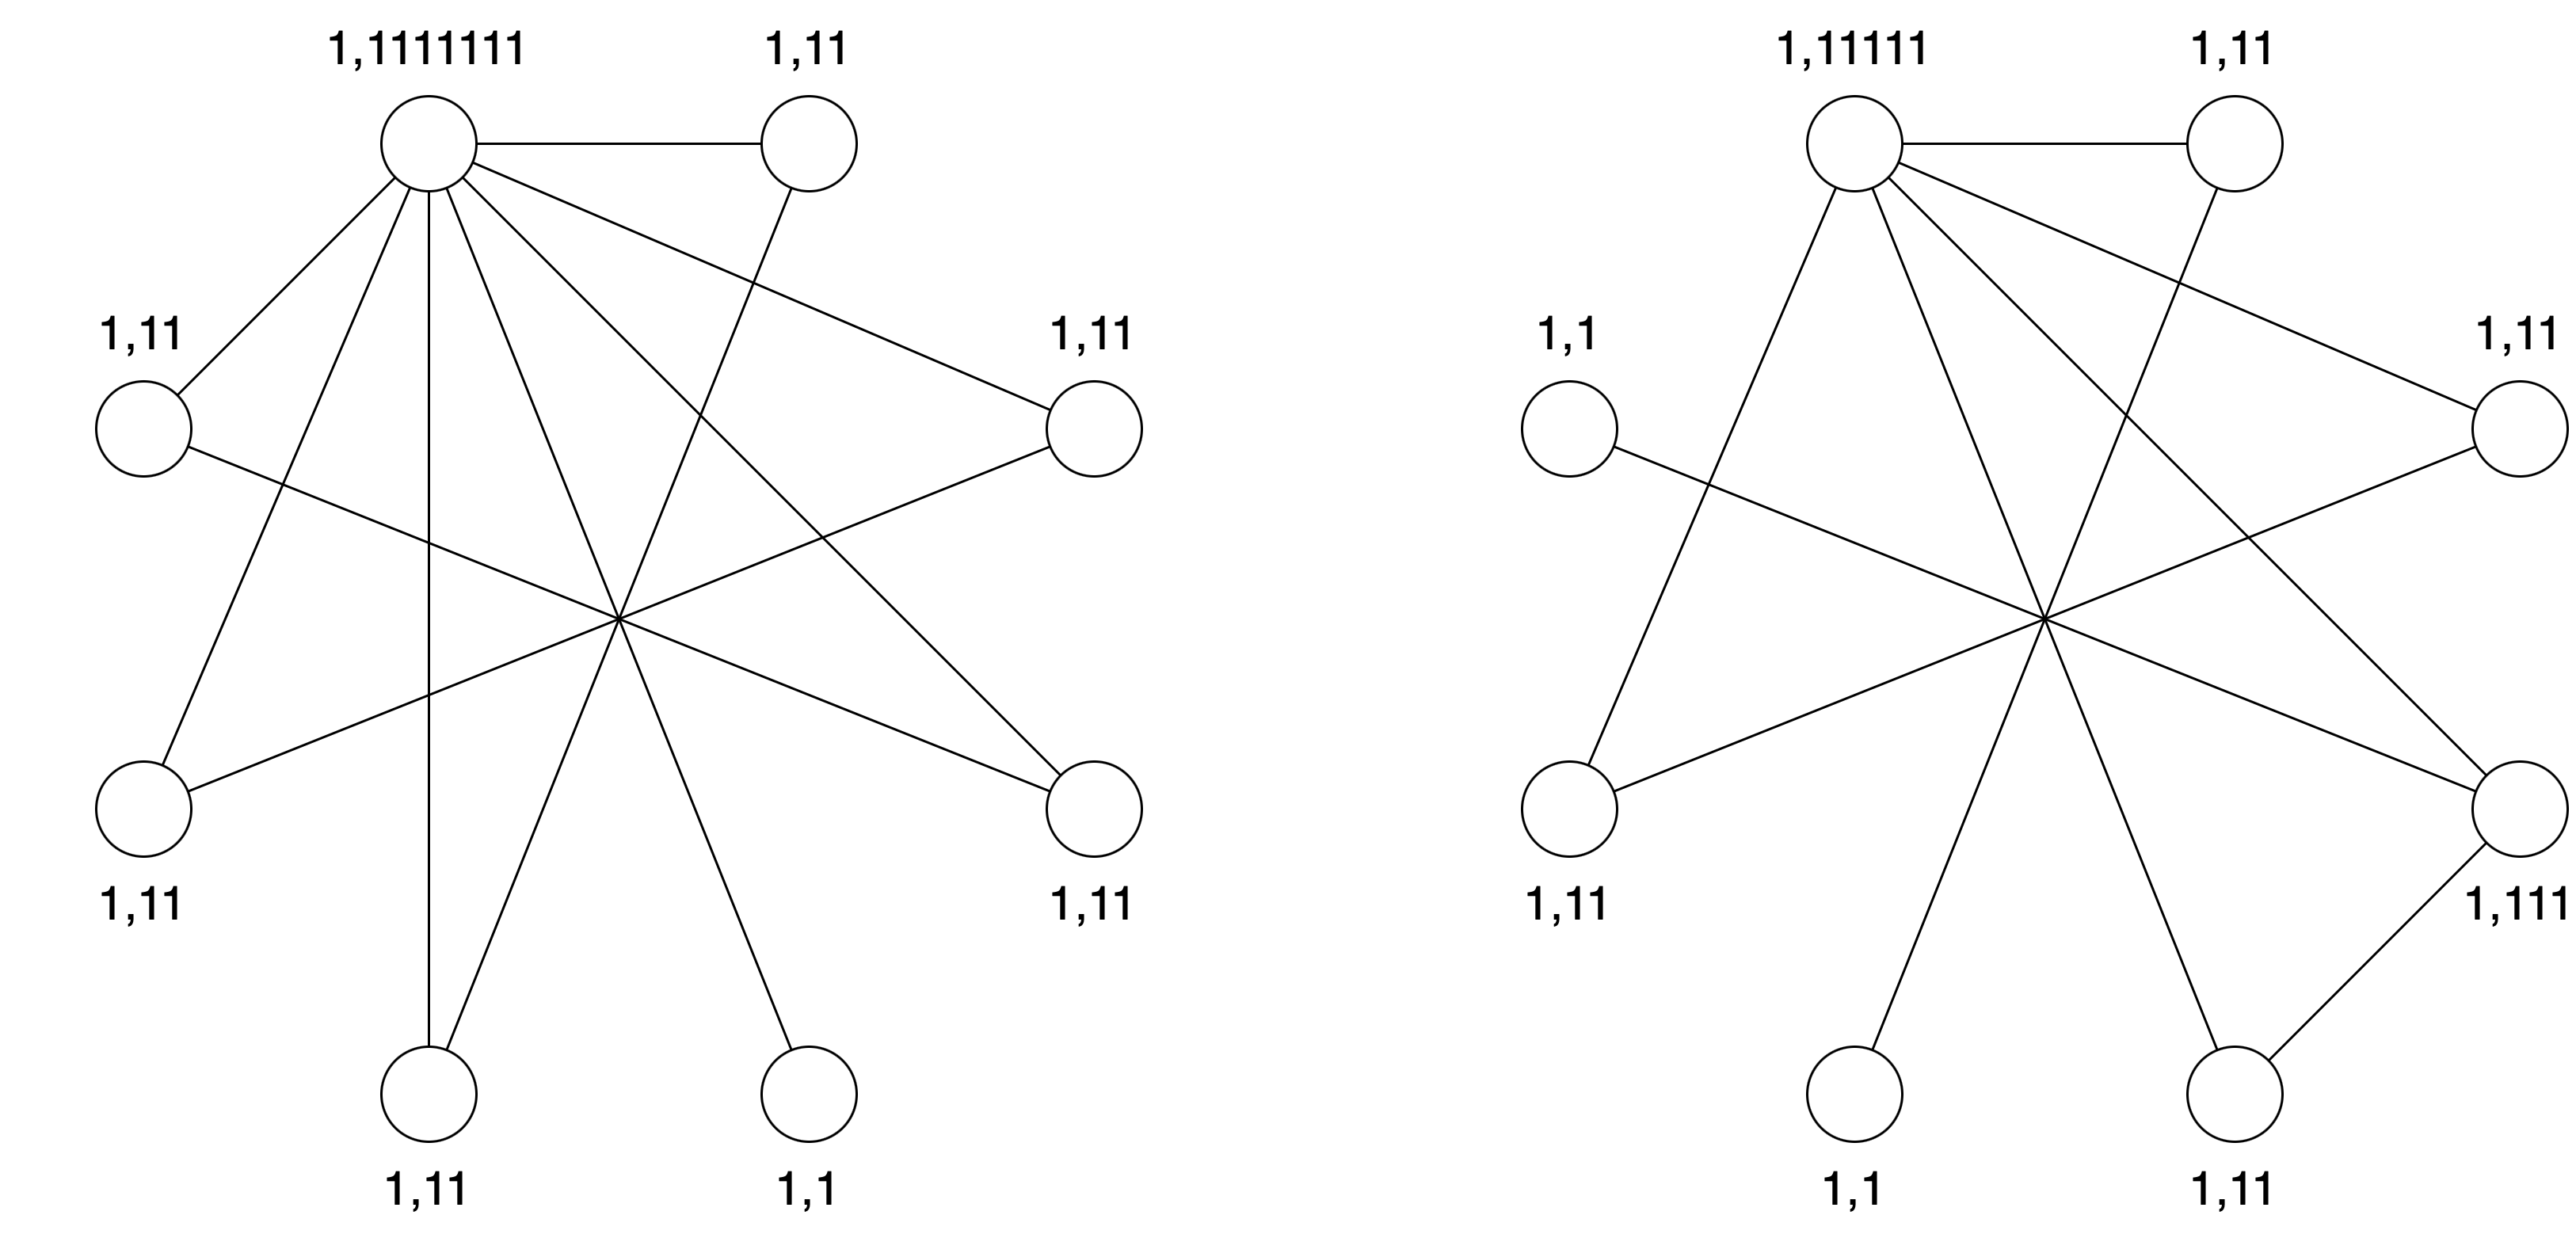
\includegraphics[width=\textwidth]{task13-1.png}
    \caption{Начальная раскраска графов и агрегирование цветов смежных вершин}
    \label{fig:13-1}
\end{figure}

Определим хэш-функцию $H$ на полученных агрегированных цветах (\ref{tbl:13-1}).
\begin{table}[h!]
    \caption{Значения хэш-функции $H$ на цветах с рисунка \ref{fig:13-1}}
    \label{tbl:13-1}
    \begin{tabularx}{\textwidth}{|X|X|}
        \hline
        Цвет $c$ & $H(c)$ \\
        \hline
        1,1 & 2 \\
        \hline
        1,11 & 3 \\
        \hline
        1,111 & 4 \\
        \hline
        1,11111 & 5 \\
        \hline
        1,1111111  & 6 \\
        \hline
    \end{tabularx}
\end{table}

Заменим старые цвета на полученные (рис. \ref{fig:13-2}) и так же сразу агрегируем цвета смежных вершин.
 
\begin{figure}[h!]
    \centering
    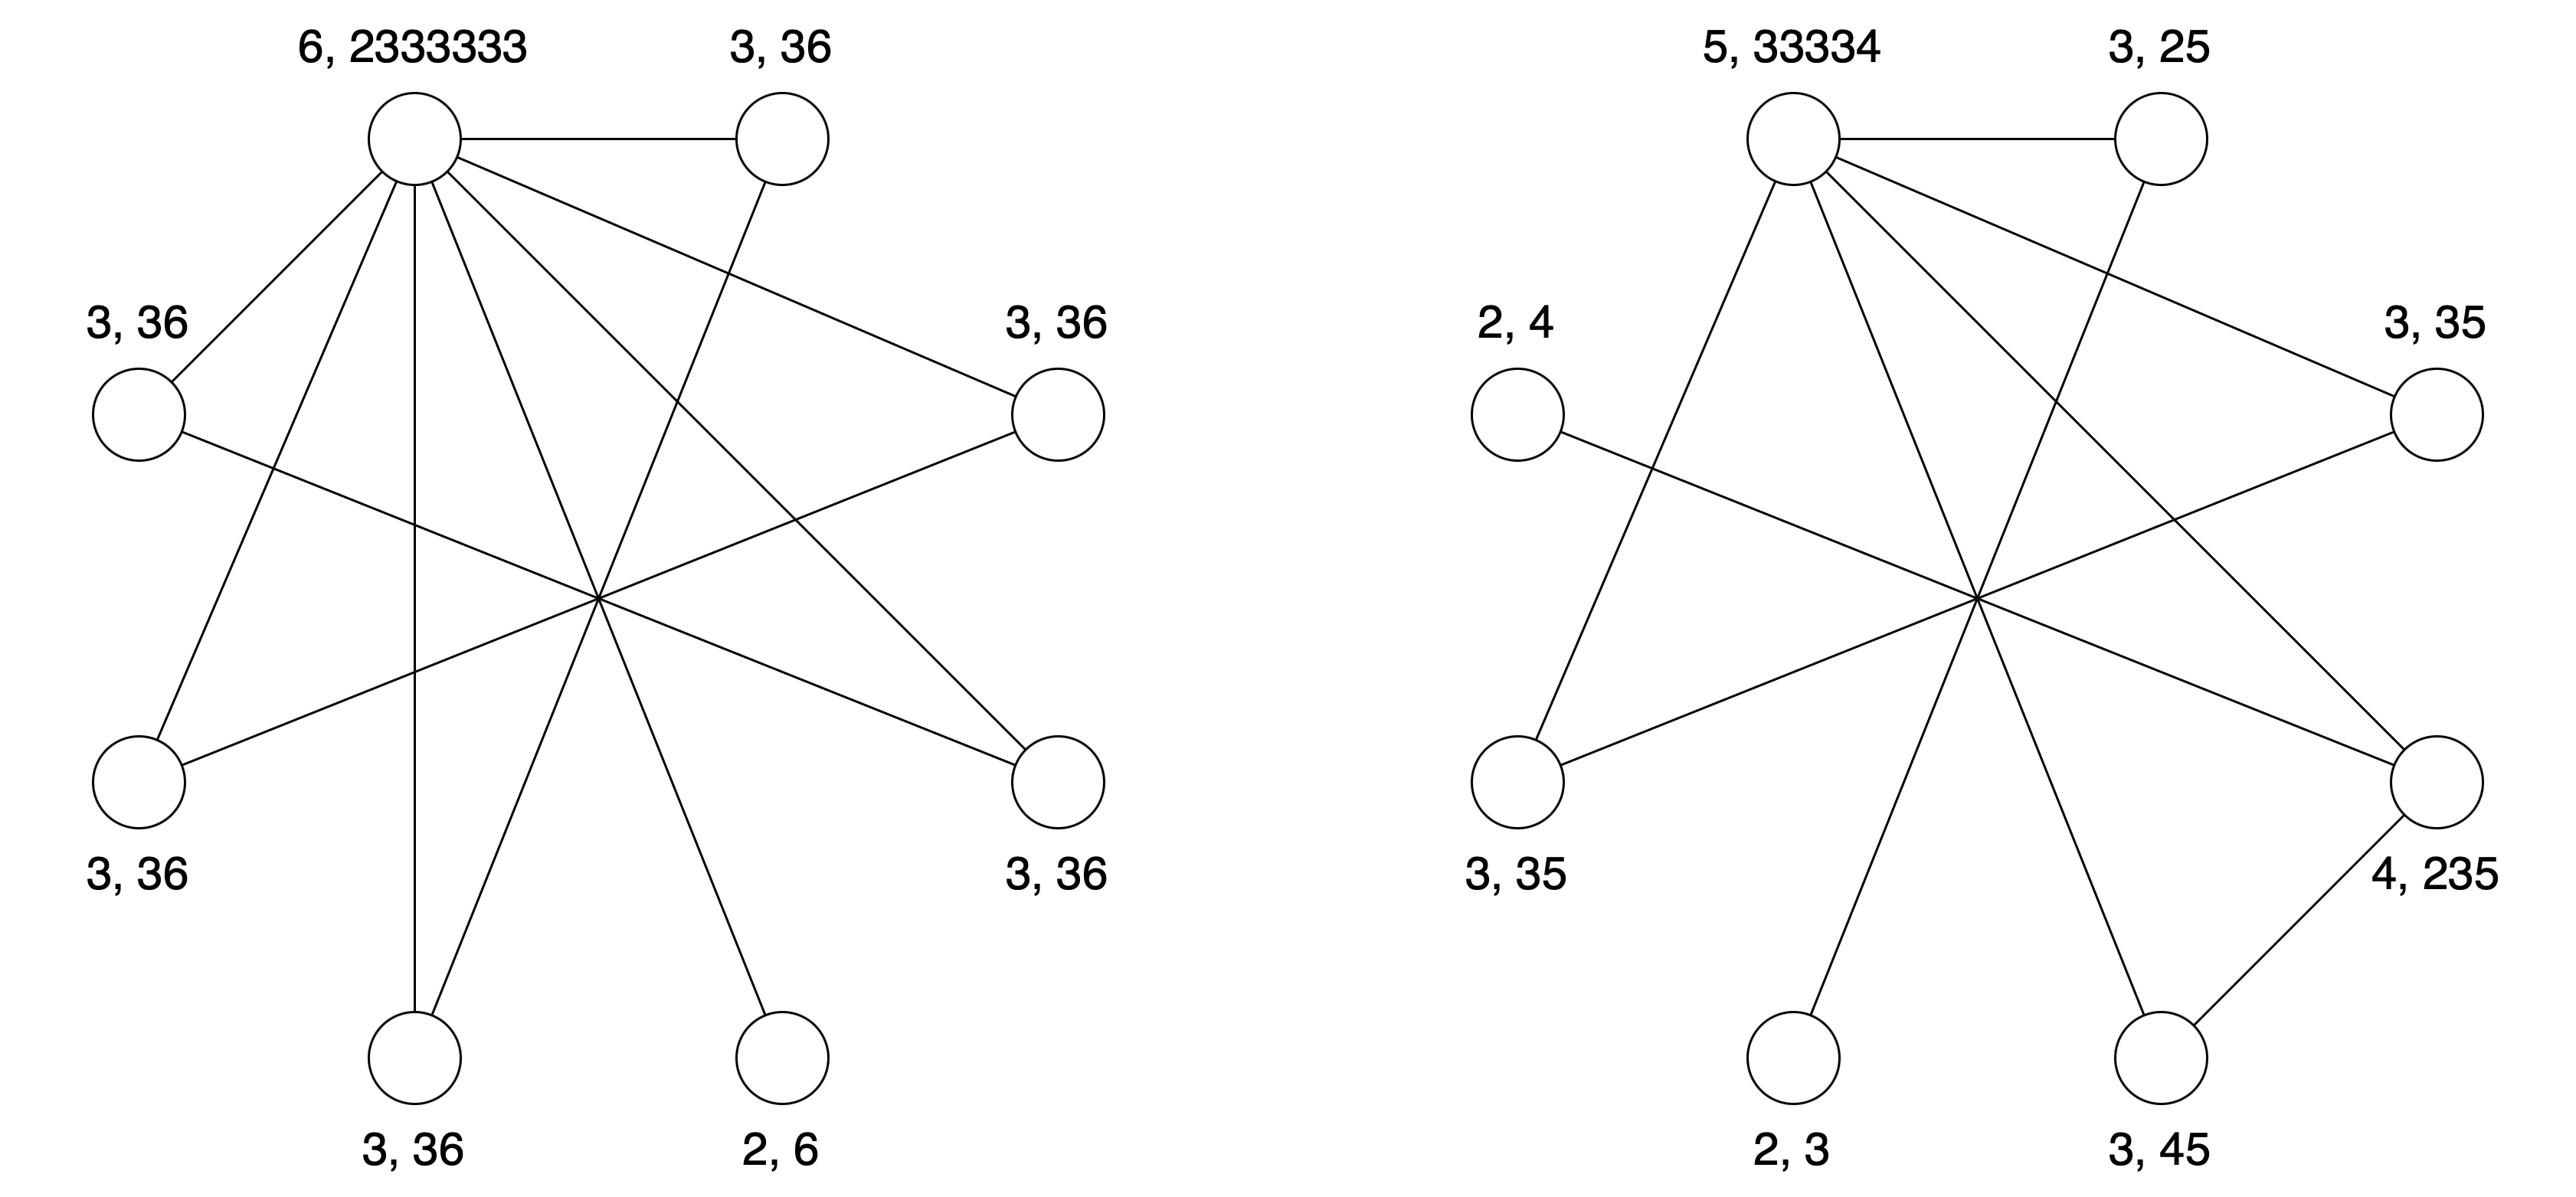
\includegraphics[width=\textwidth]{task13-2.png}
    \caption{Раскраска графов и агрегирование цветов смежных вершин на втором шаге}
    \label{fig:13-2}
\end{figure}

Доопределим хэш-функцию на полученных цветах (\ref{tbl:13-2}).
\begin{table}[h!]
    \caption{Значения хэш-функции $H$ на цветах с рисунка \ref{fig:13-2}}
    \label{tbl:13-2}
    \begin{tabularx}{\textwidth}{|X|X|}
        \hline
        Цвет $c$ & $H(c)$ \\
        \hline
        2,3 & 7\\
        \hline
        2,4 & 8\\
        \hline
        2,6 & 9\\
        \hline
        3,25 & 10\\
        \hline
        3,35 & 11\\
        \hline
        3,36 & 12\\
        \hline
        3,45 & 13\\
        \hline
        4,235 & 14\\
        \hline
        5,33334 & 15\\
        \hline
        6,2333333 & 16\\
        \hline
    \end{tabularx}
\end{table}

Повторим замену цветов (рис. \ref{fig:13-3}) и заметим, что при последующих заменах получится так, что
цвета, одинаково поменявшиеся на шаге 3, меняются одинаково и на последующих шагах, а поменявшиеся по-разному
--- меняются по-разному. Таким образом, алгоритм сошелся.
 
\begin{figure}[h!]
    \centering
    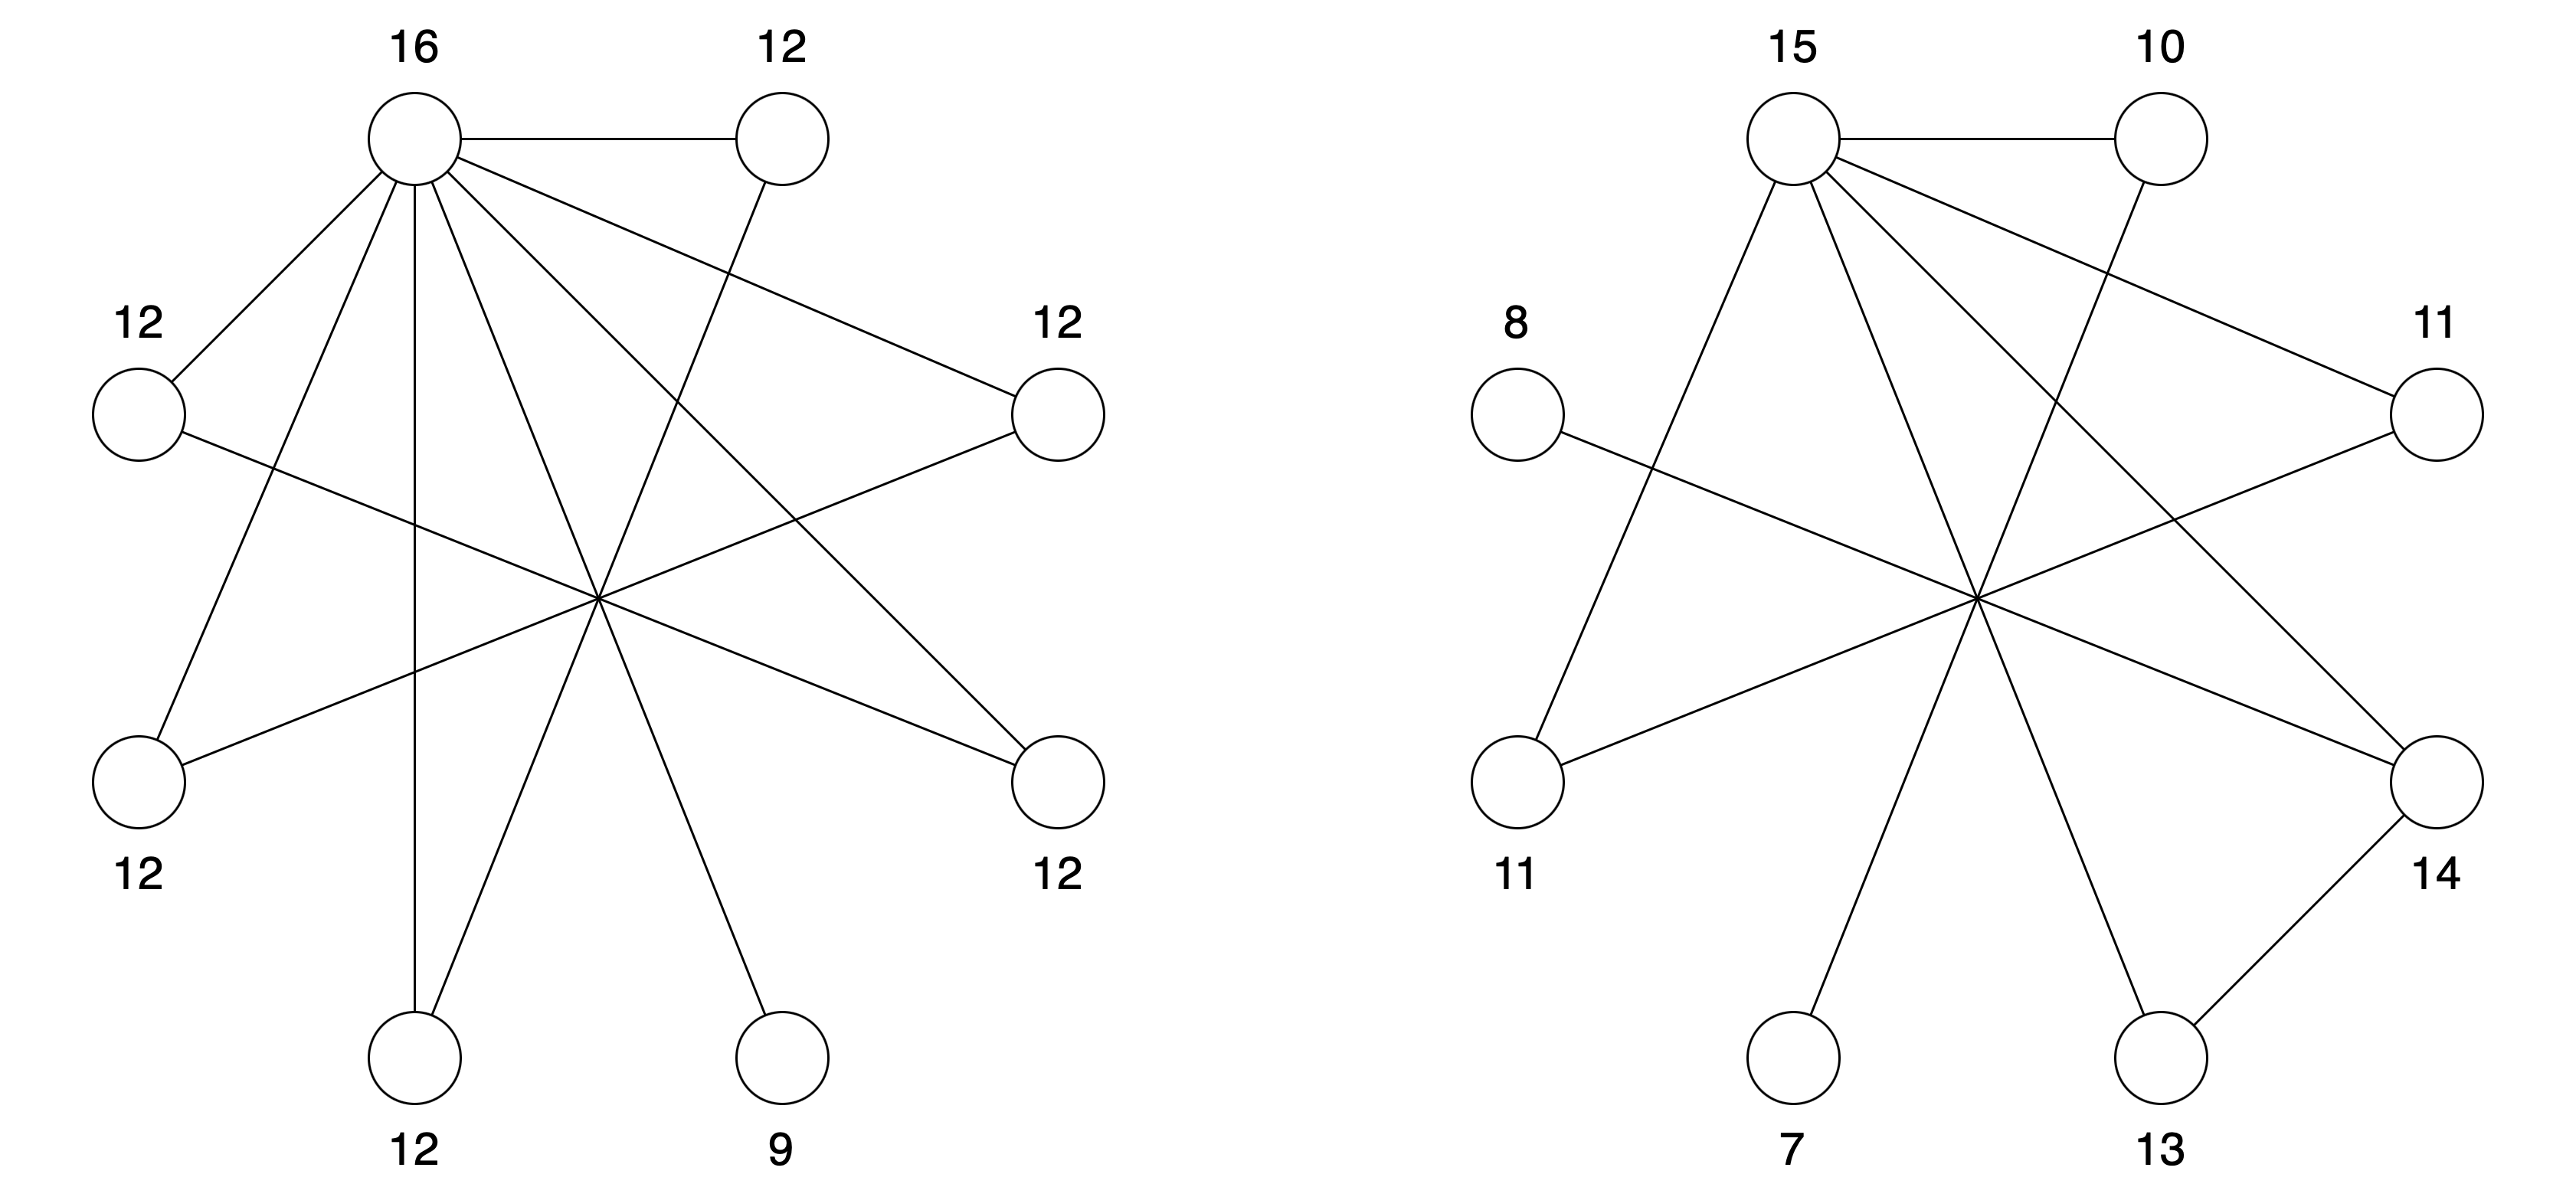
\includegraphics[width=\textwidth]{task13-3.png}
    \caption{Раскраска графов на третьем шаге}
    \label{fig:13-3}
\end{figure}

Теперь вычислим значение ядра. Для начала посчитаем количество вершин с конкретными цветами и составим
из этого векторы:
\begin{equation}
\begin{split}
    \phi_1 & = \begin{Vmatrix} 8 & 1 & 6 & 0 & 0 & 1 & 0 & 0 & 1 & 0 & 0 & 6 & 0 & 0 & 0 & 1 \end{Vmatrix} \\
    \phi_2 & = \begin{Vmatrix} 8 & 2 & 4 & 1 & 1 & 0 & 1 & 1 & 0 & 1 & 2 & 0 & 1 & 1 & 1 & 0 \end{Vmatrix}
\end{split}
\end{equation}

Непосредственно значение ядра:
\begin{equation}
    K(G_1, G_2) = \langle \phi_1, \phi_2 \rangle = 90.
\end{equation}

\Answer{$K(G_1, G_2) = 90$.}

\mysection{Задание 14}

В данном задании опишу часть моей ВКР в бакалавриате, так как она как раз посвящена обучению с подкреплением
(если точнее, то глубокому обучению с подкреплением). Решалась задача прогнозирования трех параметров 
производных финансовых инструментов (на примере фьючерсов): цены, объема и открытого интереса.

Модель содержит некоторое количество агентов --- математических моделей игроков срочного рынка, которых
характеризует неизменная в течение процесса моделирования стратегия (пара функций $(\phi_k, f_k)$, где
$k$ --- номер агента), в соответствии с ней агент выставляет заявки, и изменяющееся внутреннее состояние 
(на $t$-м шаге модельного времени вектор внутреннего состояния выглядит так: $s_k(t) = (m_k(t), z_k(t))$,
где $k$ --- номер агента, $m_k(t)$ --- остаток денег у $k$-го агента к моменту начала $t$-го шага времени,
$z_k(t)$ --- зависящие от конкретной стратегии агента значения). 

Средой является абстракция ранка (стакан, модель клирингового центра и пр.).

На каждом $t$-м шаге модельного времени $k$-й агент (для всех $k$) может разместить некоторое количество $n^+_k(t)$ 
заявок на покупку или некоторое количество $n^-_k(t)$ заявок на продажу. Данные количества не могут превысить 
максимально возможное количество заявок, которые может разместить $k$-й агент на $t$-м шаге:
\begin{equation}
    n^{max}_k(t) = \left\lfloor \frac{m_k(t)}{c} \right\rfloor,
\end{equation}
где $c$ --- величина, называемая гарантийным обеспечением (для упрощения модели она принята постоянной на
протяжении всего времени моделирования).

При помощи функции $f_k$ агент вырабатывает значение готовности $r_k(t) \in [0; 1]$, а далее желаемое количество 
заявок рассчитывается следующим образом:
\begin{itemize}
    \item если $r_k(t) \in [-1; 0)$, то: $n^-_k(t) = \lfloor n^{max}_k(t) \cdot |r_k(t)| \rfloor$, $n^+_k(t) = 0$;
    \item если $r_k(t) \in (0; 1]$, то: $n^+_k(t) = \lfloor n^{max}_k(t) \cdot r_k(t) \rfloor$, $n^-_k(t) = 0$;
    \item если $r_k(t) = 0$, то агент выходит из рынка.
\end{itemize}

Цена в заявке формируется следующим образом: $p_k(t) = \lfloor \hat{p}(t - 1) (1 + \omega r_k(t)) \rfloor$,
где $\hat{p}(t - 1)$ --- смоделированная (выход модели) на шаге $t - 1$ цена, $\omega \in (0, 1]$ --- неизменный
в течение моделирования параметр модели.

При этом в действительности на $t$-м шаге $k$-агент размещает следующее количество заявок (заметим, что оно
не всегда равно желаемому, чтобы учесть уже размещенные, но еще не закрытые):
\begin{equation}
    n_k(t) = \sgn\left(\xi_k(t)\right) \min\left(n^{max}_k(t), \xi_k(t)\right),
\end{equation}
где $\xi_k(t) = |n^{max}_k(t) |r_k(t)| - o_k(t) - n^+_k(t) + n^-_k(t)|$, $o_k(t)$ --- количество действующих
на момент начала шага $t$ контрактов для агента $k$.

На этом описание действий агента не завершается. Перед вычислением значения $r_k(t)$ агент обновляет свою внутреннее
состояние при помощи функции $\phi_k$ на основе предыдущего внутреннего состояния $s_k(t - 1)$, 
смоделированных цены $\hat{p}(t - 1)$, объема $\hat{v}(t - 1)$ и открытого интереса $\hat{a}(t - 1)$,
а также вектора параметров модели $\vec{x}_k$ (данные параметры как раз и подбираются в ходе обучения модели).

После размещения заявок наступает клиринговая фаза, и вычисляются значения смоделированных цены $\hat{p}(t)$, 
объема $\hat{v}(t)$ и открытого интереса $\hat{a}(t)$ (функции их вычисления приводить не буду в силу их 
нетривиальности).

Оптимизируется функция $L(P, V, A, \vec{x}) = \sum_t \mathcal{F}(\rho(p_t, \hat{p}(t)), \rho(v_t, \hat{v}(t)),
\rho(a_t, \hat{a}(t)))$, где $\rho$ --- метрика в $\mathbb{R} ^ 2$, $\mathcal{F}$ --- функция, которая прямо
пропорциональна каждому своему аргументу (например, среднее трех входных значений), $P$, $V$, $A$ --- исходные
временные ряды цен, объемов и открытого интереса (обучающая выборка).

Таким образом, задачей является нахождение:
\begin{equation}
    \vec{x}^\ast = \argmin_{\vec{x}} L(P, V, A, \vec{x}),
\end{equation}
где $\vec{x} = \begin{Vmatrix}
    \vec{x_1} & \cdots & \vec{x}_K
\end{Vmatrix}$.

Агенты в модели имеют различные стратегии, основанные на реальном поведении игроков на срочном рынке. Примером,
может служить использование индикаторов, например, MACD или полос Боллинджера\footnotemark. Данные стратегии
определяют вектор параметров $z_k(t)$, хранимых во внутреннем состоянии, а также конкретный вид функций
$\phi_k$ и $f_k$.

\footnotetext{Подробнее: Кауфман П. Системы и методы биржевой торговли ; Пер. с англ. --- М. : Альпина 
    Паблишер, 2017 --- 1279 с.}

Вознаграждение агента обратно пропорционально значению функции $\mathcal{F}$ на рассматриваемом шаге. При
этом если по сравнению с предыдущим шагом была улучшена точность прогнозирования, то величина является
положительной, а если точность ухудшилась, то --- отрицательной. При этом отдельно рассматривается случай
равенства нулю расстояний до обучающих данных: в этом случае вознаграждение фиксированное положительное
(использовалось значение 100).

Задача обучения решалась методом градиента стратегии, так как значения состояния фактически ограничений не
имеют. Элементы вектора действий (количества размещаемых заявок) хоть и ограничены целочисленными значениям,
но было введено допущение в виде трактовки пространства действий как $\mathbb{R}^K$, где $K$ --- количество
задействованных агентов. В силу того, что процесс моделирования может продолжаться сколь угодно долго,
задача считается непрерывной. Суть метода состоит в нахождении некоторых приближений функций ценности 
$v_\pi(s)$ (это математическое ожидание дохода при начале работы в состоянии $s$ и следовании стратегии
$\pi$) и самой стратегии $\pi(a | s)$ (выражающей вероятность принять действие $a$ при нахождении в
состоянии $s$), где через $a$ традиционно для публикаций по обучению с подкреплением обозначается действие.
Приближения находятся при помощи параметризации (а параметрами и выступают векторы $\vec{x}_k$).

В качестве <<истинной>> стратегии была выбрана многомерная гауссова: $\pi(a | s) =
\prod_{j = 1}^{K} \mathcal{N}(\mu_j(s), \sigma^2_j(s))$ (это предположение). Для решения был выбран 
метод <<исполнитель-критик>>.

При этом следует отметить, что используемые стратегии на основе индикаторов не являются дифференцируемыми
по вектору параметров (а это необходимо для метода <<исполнитель-критик>>), в связи с чем было принято 
решение аппроксимировать их при помощи нейронной сети (сеть вырабатывает на выходе весь вектор действий).
Функция ценности состояния также аппроксимируется нейронной сетью. Следует отметить, что обучение проходит
в два этапа: на первом запускается симуляция, в ходе которой нейронные сети обучаются аппроксимировать
параметризованные функцию стратегии и функцию ценности состояния (параметры являются входами нейронных
сетей), то есть устанавливается приближенная зависимость результатов функций от входных
данных и параметров модели рынка. На втором же этапе обучения (второй симуляции) происходит подбор
параметров самой модели с использованием полученных приближений (которые, несомненно, являются дифференцируемыми
по параметрам модели) по методу <<исполнитель-критик>>. Найденные на втором этапе параметры модели
считаются оптимальными и определяют оптимальную стратегию (строго говоря, --- ее приближение). \\

\mysection{Задание 15}

:(

\pagebreak
\mysection{Приложение А. Таблицы с перечислением кратчайших путей между вершинами графа из задачи 10}

\begin{table}[h!]
    \caption{Пути из вершины $1$ в другие вершины.}
    \label{tbl:10-1}
    \begin{tabularx}{\textwidth}{|X|X|X|}
        \hline 
        Целевая вершина & Кратчайшие пути & Доля путей через 18 \\
        \hline 
        $2$ & \begin{tabular}{@{}l@{}} $[1, 3, 2]$ \\ \end{tabular} & $0/1$ \\
        \hline
        $3$ & \begin{tabular}{@{}l@{}} $[1, 3]$ \\ \end{tabular} & $0/1$ \\
        \hline
        $4$ & \begin{tabular}{@{}l@{}} $[1, 3, 6, 4]$ \\ \end{tabular} & $0/1$ \\
        \hline
        $5$ & \begin{tabular}{@{}l@{}} $[1, 3, 6, 5]$ \\ \end{tabular} & $0/1$ \\
        \hline
        $6$ & \begin{tabular}{@{}l@{}} $[1, 3, 6]$ \\ \end{tabular} & $0/1$ \\
        \hline
        $7$ & \begin{tabular}{@{}l@{}} $[1, 3, 7]$ \\ \end{tabular} & $0/1$ \\
        \hline
        $8$ & \begin{tabular}{@{}l@{}} $[1, 3, 7, 8]$ \\ \end{tabular} & $0/1$ \\
        \hline
        $9$ & \begin{tabular}{@{}l@{}} $[1, 3, 9]$ \\ \end{tabular} & $0/1$ \\
        \hline
        $10$ & \begin{tabular}{@{}l@{}} $[1, 3, 6, 10]$ \\ \end{tabular} & $0/1$ \\
        \hline
        $11$ & \begin{tabular}{@{}l@{}} $[1, 3, 6, 10, 11]$ \\ \end{tabular} & $0/1$ \\
        \hline
        $12$ & \begin{tabular}{@{}l@{}} $[1, 3, 9, 13, 12]$ \\ \end{tabular} & $0/1$ \\
        \hline
        $13$ & \begin{tabular}{@{}l@{}} $[1, 3, 9, 13]$ \\ \end{tabular} & $0/1$ \\
        \hline
        $14$ & \begin{tabular}{@{}l@{}} $[1, 3, 9, 14]$ \\ \end{tabular} & $0/1$ \\
        \hline
        $15$ & \begin{tabular}{@{}l@{}} $[1, 3, 9, 13, 15]$ \\  $[1, 3, 9, 14, 15]$ \\ \end{tabular} & $0/2$ \\
        \hline
        $16$ & \begin{tabular}{@{}l@{}} $[1, 3, 6, 10, 16]$ \\ \end{tabular} & $0/1$ \\
        \hline
        $17$ & \begin{tabular}{@{}l@{}} $[1, 3, 9, 13, 15, 18, 17]$ \\  $[1, 3, 9, 14, 15, 18, 17]$ \\  $[1, 3, 9, 14, 19, 18, 17]$ \\ \end{tabular} & $3/3$ \\
        \hline
        $19$ & \begin{tabular}{@{}l@{}} $[1, 3, 9, 14, 19]$ \\ \end{tabular} & $0/1$ \\
        \hline
        $20$ & \begin{tabular}{@{}l@{}} $[1, 3, 9, 14, 19, 20]$ \\ \end{tabular} & $0/1$ \\
        \hline
    \end{tabularx}
\end{table}

\begin{table}[h!]
    \caption{Пути из вершины $2$ в другие вершины.}
    \label{tbl:10-2}
    \begin{tabularx}{\textwidth}{|X|X|X|}
        \hline 
        Целевая вершина & Кратчайшие пути & Доля путей через 18 \\
        \hline 
        $3$ & \begin{tabular}{@{}l@{}} $[2, 3]$ \\ \end{tabular} & $0/1$ \\
        \hline
        $4$ & \begin{tabular}{@{}l@{}} $[2, 3, 6, 4]$ \\ \end{tabular} & $0/1$ \\
        \hline
        $5$ & \begin{tabular}{@{}l@{}} $[2, 3, 6, 5]$ \\ \end{tabular} & $0/1$ \\
        \hline
        $6$ & \begin{tabular}{@{}l@{}} $[2, 3, 6]$ \\ \end{tabular} & $0/1$ \\
        \hline
        $7$ & \begin{tabular}{@{}l@{}} $[2, 3, 7]$ \\ \end{tabular} & $0/1$ \\
        \hline
        $8$ & \begin{tabular}{@{}l@{}} $[2, 3, 7, 8]$ \\ \end{tabular} & $0/1$ \\
        \hline
        $9$ & \begin{tabular}{@{}l@{}} $[2, 3, 9]$ \\ \end{tabular} & $0/1$ \\
        \hline
        $10$ & \begin{tabular}{@{}l@{}} $[2, 3, 6, 10]$ \\ \end{tabular} & $0/1$ \\
        \hline
        $11$ & \begin{tabular}{@{}l@{}} $[2, 3, 6, 10, 11]$ \\ \end{tabular} & $0/1$ \\
        \hline
        $12$ & \begin{tabular}{@{}l@{}} $[2, 3, 9, 13, 12]$ \\ \end{tabular} & $0/1$ \\
        \hline
        $13$ & \begin{tabular}{@{}l@{}} $[2, 3, 9, 13]$ \\ \end{tabular} & $0/1$ \\
        \hline
        $14$ & \begin{tabular}{@{}l@{}} $[2, 3, 9, 14]$ \\ \end{tabular} & $0/1$ \\
        \hline
        $15$ & \begin{tabular}{@{}l@{}} $[2, 3, 9, 13, 15]$ \\  $[2, 3, 9, 14, 15]$ \\ \end{tabular} & $0/2$ \\
        \hline
        $16$ & \begin{tabular}{@{}l@{}} $[2, 3, 6, 10, 16]$ \\ \end{tabular} & $0/1$ \\
        \hline
        $17$ & \begin{tabular}{@{}l@{}} $[2, 3, 9, 13, 15, 18, 17]$ \\  $[2, 3, 9, 14, 15, 18, 17]$ \\  $[2, 3, 9, 14, 19, 18, 17]$ \\ \end{tabular} & $3/3$ \\
        \hline
        $19$ & \begin{tabular}{@{}l@{}} $[2, 3, 9, 14, 19]$ \\ \end{tabular} & $0/1$ \\
        \hline
        $20$ & \begin{tabular}{@{}l@{}} $[2, 3, 9, 14, 19, 20]$ \\ \end{tabular} & $0/1$ \\
        \hline
    \end{tabularx}
\end{table}
\begin{table}[h!]
    \caption{Пути из вершины $3$ в другие вершины.}
    \label{tbl:10-3}
    \begin{tabularx}{\textwidth}{|X|X|X|}
        \hline 
        Целевая вершина & Кратчайшие пути & Доля путей через 18 \\
        \hline 
        $4$ & \begin{tabular}{@{}l@{}} $[3, 6, 4]$ \\ \end{tabular} & $0/1$ \\
        \hline
        $5$ & \begin{tabular}{@{}l@{}} $[3, 6, 5]$ \\ \end{tabular} & $0/1$ \\
        \hline
        $6$ & \begin{tabular}{@{}l@{}} $[3, 6]$ \\ \end{tabular} & $0/1$ \\
        \hline
        $7$ & \begin{tabular}{@{}l@{}} $[3, 7]$ \\ \end{tabular} & $0/1$ \\
        \hline
        $8$ & \begin{tabular}{@{}l@{}} $[3, 7, 8]$ \\ \end{tabular} & $0/1$ \\
        \hline
        $9$ & \begin{tabular}{@{}l@{}} $[3, 9]$ \\ \end{tabular} & $0/1$ \\
        \hline
        $10$ & \begin{tabular}{@{}l@{}} $[3, 6, 10]$ \\ \end{tabular} & $0/1$ \\
        \hline
        $11$ & \begin{tabular}{@{}l@{}} $[3, 6, 10, 11]$ \\ \end{tabular} & $0/1$ \\
        \hline
        $12$ & \begin{tabular}{@{}l@{}} $[3, 9, 13, 12]$ \\ \end{tabular} & $0/1$ \\
        \hline
        $13$ & \begin{tabular}{@{}l@{}} $[3, 9, 13]$ \\ \end{tabular} & $0/1$ \\
        \hline
        $14$ & \begin{tabular}{@{}l@{}} $[3, 9, 14]$ \\ \end{tabular} & $0/1$ \\
        \hline
        $15$ & \begin{tabular}{@{}l@{}} $[3, 9, 13, 15]$ \\  $[3, 9, 14, 15]$ \\ \end{tabular} & $0/2$ \\
        \hline
        $16$ & \begin{tabular}{@{}l@{}} $[3, 6, 10, 16]$ \\ \end{tabular} & $0/1$ \\
        \hline
        $17$ & \begin{tabular}{@{}l@{}} $[3, 9, 13, 15, 18, 17]$ \\  $[3, 9, 14, 15, 18, 17]$ \\  $[3, 9, 14, 19, 18, 17]$ \\ \end{tabular} & $3/3$ \\
        \hline
        $19$ & \begin{tabular}{@{}l@{}} $[3, 9, 14, 19]$ \\ \end{tabular} & $0/1$ \\
        \hline
        $20$ & \begin{tabular}{@{}l@{}} $[3, 9, 14, 19, 20]$ \\ \end{tabular} & $0/1$ \\
        \hline
    \end{tabularx}
\end{table}
\begin{table}[h!]
    \caption{Пути из вершины $4$ в другие вершины.}
    \label{tbl:10-4}
    \begin{tabularx}{\textwidth}{|X|X|X|}
        \hline 
        Целевая вершина & Кратчайшие пути & Доля путей через 18 \\
        \hline 
        $5$ & \begin{tabular}{@{}l@{}} $[4, 6, 5]$ \\ \end{tabular} & $0/1$ \\
        \hline
        $6$ & \begin{tabular}{@{}l@{}} $[4, 6]$ \\ \end{tabular} & $0/1$ \\
        \hline
        $7$ & \begin{tabular}{@{}l@{}} $[4, 6, 3, 7]$ \\  $[4, 6, 9, 7]$ \\ \end{tabular} & $0/2$ \\
        \hline
        $8$ & \begin{tabular}{@{}l@{}} $[4, 6, 3, 7, 8]$ \\  $[4, 6, 9, 7, 8]$ \\ \end{tabular} & $0/2$ \\
        \hline
        $9$ & \begin{tabular}{@{}l@{}} $[4, 6, 9]$ \\ \end{tabular} & $0/1$ \\
        \hline
        $10$ & \begin{tabular}{@{}l@{}} $[4, 6, 10]$ \\ \end{tabular} & $0/1$ \\
        \hline
        $11$ & \begin{tabular}{@{}l@{}} $[4, 6, 10, 11]$ \\ \end{tabular} & $0/1$ \\
        \hline
        $12$ & \begin{tabular}{@{}l@{}} $[4, 6, 9, 13, 12]$ \\ \end{tabular} & $0/1$ \\
        \hline
        $13$ & \begin{tabular}{@{}l@{}} $[4, 6, 9, 13]$ \\ \end{tabular} & $0/1$ \\
        \hline
        $14$ & \begin{tabular}{@{}l@{}} $[4, 6, 9, 14]$ \\  $[4, 6, 10, 14]$ \\ \end{tabular} & $0/2$ \\
        \hline
        $15$ & \begin{tabular}{@{}l@{}} $[4, 6, 9, 13, 15]$ \\  $[4, 6, 9, 14, 15]$ \\  $[4, 6, 10, 14, 15]$ \\  $[4, 6, 10, 16, 15]$ \\ \end{tabular} & $0/4$ \\
        \hline
        $16$ & \begin{tabular}{@{}l@{}} $[4, 6, 10, 16]$ \\ \end{tabular} & $0/1$ \\
        \hline
        $17$ & \begin{tabular}{@{}l@{}} $[4, 6, 9, 13, 15, 18, 17]$ \\  $[4, 6, 9, 14, 15, 18, 17]$ \\  $[4, 6, 10, 14, 15, 18, 17]$ \\  $[4, 6, 10, 16, 15, 18, 17]$ \\  $[4, 6, 9, 14, 19, 18, 17]$ \\  $[4, 6, 10, 14, 19, 18, 17]$ \\  $[4, 6, 10, 16, 19, 18, 17]$ \\ \end{tabular} & $7/7$ \\
        \hline
        $19$ & \begin{tabular}{@{}l@{}} $[4, 6, 9, 14, 19]$ \\  $[4, 6, 10, 14, 19]$ \\  $[4, 6, 10, 16, 19]$ \\ \end{tabular} & $0/3$ \\
        \hline
        $20$ & \begin{tabular}{@{}l@{}} $[4, 6, 9, 14, 19, 20]$ \\  $[4, 6, 10, 14, 19, 20]$ \\  $[4, 6, 10, 16, 19, 20]$ \\ \end{tabular} & $0/3$ \\
        \hline
    \end{tabularx}
\end{table}
\begin{table}[h!]
    \caption{Пути из вершины $5$ в другие вершины.}
    \label{tbl:10-5}
    \begin{tabularx}{\textwidth}{|X|X|X|}
        \hline 
        Целевая вершина & Кратчайшие пути & Доля путей через 18 \\
        \hline 
        $6$ & \begin{tabular}{@{}l@{}} $[5, 6]$ \\ \end{tabular} & $0/1$ \\
        \hline
        $7$ & \begin{tabular}{@{}l@{}} $[5, 6, 3, 7]$ \\  $[5, 6, 9, 7]$ \\ \end{tabular} & $0/2$ \\
        \hline
        $8$ & \begin{tabular}{@{}l@{}} $[5, 6, 3, 7, 8]$ \\  $[5, 6, 9, 7, 8]$ \\ \end{tabular} & $0/2$ \\
        \hline
        $9$ & \begin{tabular}{@{}l@{}} $[5, 6, 9]$ \\ \end{tabular} & $0/1$ \\
        \hline
        $10$ & \begin{tabular}{@{}l@{}} $[5, 6, 10]$ \\ \end{tabular} & $0/1$ \\
        \hline
        $11$ & \begin{tabular}{@{}l@{}} $[5, 6, 10, 11]$ \\ \end{tabular} & $0/1$ \\
        \hline
        $12$ & \begin{tabular}{@{}l@{}} $[5, 6, 9, 13, 12]$ \\ \end{tabular} & $0/1$ \\
        \hline
        $13$ & \begin{tabular}{@{}l@{}} $[5, 6, 9, 13]$ \\ \end{tabular} & $0/1$ \\
        \hline
        $14$ & \begin{tabular}{@{}l@{}} $[5, 6, 9, 14]$ \\  $[5, 6, 10, 14]$ \\ \end{tabular} & $0/2$ \\
        \hline
        $15$ & \begin{tabular}{@{}l@{}} $[5, 6, 9, 13, 15]$ \\  $[5, 6, 9, 14, 15]$ \\  $[5, 6, 10, 14, 15]$ \\  $[5, 6, 10, 16, 15]$ \\ \end{tabular} & $0/4$ \\
        \hline
        $16$ & \begin{tabular}{@{}l@{}} $[5, 6, 10, 16]$ \\ \end{tabular} & $0/1$ \\
        \hline
        $17$ & \begin{tabular}{@{}l@{}} $[5, 6, 9, 13, 15, 18, 17]$ \\  $[5, 6, 9, 14, 15, 18, 17]$ \\  $[5, 6, 10, 14, 15, 18, 17]$ \\  $[5, 6, 10, 16, 15, 18, 17]$ \\  $[5, 6, 9, 14, 19, 18, 17]$ \\  $[5, 6, 10, 14, 19, 18, 17]$ \\  $[5, 6, 10, 16, 19, 18, 17]$ \\ \end{tabular} & $7/7$ \\
        \hline
        $19$ & \begin{tabular}{@{}l@{}} $[5, 6, 9, 14, 19]$ \\  $[5, 6, 10, 14, 19]$ \\  $[5, 6, 10, 16, 19]$ \\ \end{tabular} & $0/3$ \\
        \hline
        $20$ & \begin{tabular}{@{}l@{}} $[5, 6, 9, 14, 19, 20]$ \\  $[5, 6, 10, 14, 19, 20]$ \\  $[5, 6, 10, 16, 19, 20]$ \\ \end{tabular} & $0/3$ \\
        \hline
    \end{tabularx}
\end{table}
\begin{table}[h!]
    \caption{Пути из вершины $6$ в другие вершины.}
    \label{tbl:10-6}
    \begin{tabularx}{\textwidth}{|X|X|X|}
        \hline 
        Целевая вершина & Кратчайшие пути & Доля путей через 18 \\
        \hline 
        $7$ & \begin{tabular}{@{}l@{}} $[6, 3, 7]$ \\  $[6, 9, 7]$ \\ \end{tabular} & $0/2$ \\
        \hline
        $8$ & \begin{tabular}{@{}l@{}} $[6, 3, 7, 8]$ \\  $[6, 9, 7, 8]$ \\ \end{tabular} & $0/2$ \\
        \hline
        $9$ & \begin{tabular}{@{}l@{}} $[6, 9]$ \\ \end{tabular} & $0/1$ \\
        \hline
        $10$ & \begin{tabular}{@{}l@{}} $[6, 10]$ \\ \end{tabular} & $0/1$ \\
        \hline
        $11$ & \begin{tabular}{@{}l@{}} $[6, 10, 11]$ \\ \end{tabular} & $0/1$ \\
        \hline
        $12$ & \begin{tabular}{@{}l@{}} $[6, 9, 13, 12]$ \\ \end{tabular} & $0/1$ \\
        \hline
        $13$ & \begin{tabular}{@{}l@{}} $[6, 9, 13]$ \\ \end{tabular} & $0/1$ \\
        \hline
        $14$ & \begin{tabular}{@{}l@{}} $[6, 9, 14]$ \\  $[6, 10, 14]$ \\ \end{tabular} & $0/2$ \\
        \hline
        $15$ & \begin{tabular}{@{}l@{}} $[6, 9, 13, 15]$ \\  $[6, 9, 14, 15]$ \\  $[6, 10, 14, 15]$ \\  $[6, 10, 16, 15]$ \\ \end{tabular} & $0/4$ \\
        \hline
        $16$ & \begin{tabular}{@{}l@{}} $[6, 10, 16]$ \\ \end{tabular} & $0/1$ \\
        \hline
        $17$ & \begin{tabular}{@{}l@{}} $[6, 9, 13, 15, 18, 17]$ \\  $[6, 9, 14, 15, 18, 17]$ \\  $[6, 10, 14, 15, 18, 17]$ \\  $[6, 10, 16, 15, 18, 17]$ \\  $[6, 9, 14, 19, 18, 17]$ \\  $[6, 10, 14, 19, 18, 17]$ \\  $[6, 10, 16, 19, 18, 17]$ \\ \end{tabular} & $7/7$ \\
        \hline
        $19$ & \begin{tabular}{@{}l@{}} $[6, 9, 14, 19]$ \\  $[6, 10, 14, 19]$ \\  $[6, 10, 16, 19]$ \\ \end{tabular} & $0/3$ \\
        \hline
        $20$ & \begin{tabular}{@{}l@{}} $[6, 9, 14, 19, 20]$ \\  $[6, 10, 14, 19, 20]$ \\  $[6, 10, 16, 19, 20]$ \\ \end{tabular} & $0/3$ \\
        \hline
    \end{tabularx}
\end{table}
\begin{table}[h!]
    \caption{Пути из вершины $7$ в другие вершины.}
    \label{tbl:10-7}
    \begin{tabularx}{\textwidth}{|X|X|X|}
        \hline 
        Целевая вершина & Кратчайшие пути & Доля путей через 18 \\
        \hline 
        $8$ & \begin{tabular}{@{}l@{}} $[7, 8]$ \\ \end{tabular} & $0/1$ \\
        \hline
        $9$ & \begin{tabular}{@{}l@{}} $[7, 9]$ \\ \end{tabular} & $0/1$ \\
        \hline
        $10$ & \begin{tabular}{@{}l@{}} $[7, 3, 6, 10]$ \\  $[7, 9, 6, 10]$ \\  $[7, 9, 14, 10]$ \\ \end{tabular} & $0/3$ \\
        \hline
        $11$ & \begin{tabular}{@{}l@{}} $[7, 3, 6, 10, 11]$ \\  $[7, 9, 6, 10, 11]$ \\  $[7, 9, 14, 10, 11]$ \\ \end{tabular} & $0/3$ \\
        \hline
        $12$ & \begin{tabular}{@{}l@{}} $[7, 9, 13, 12]$ \\ \end{tabular} & $0/1$ \\
        \hline
        $13$ & \begin{tabular}{@{}l@{}} $[7, 9, 13]$ \\ \end{tabular} & $0/1$ \\
        \hline
        $14$ & \begin{tabular}{@{}l@{}} $[7, 9, 14]$ \\ \end{tabular} & $0/1$ \\
        \hline
        $15$ & \begin{tabular}{@{}l@{}} $[7, 9, 13, 15]$ \\  $[7, 9, 14, 15]$ \\ \end{tabular} & $0/2$ \\
        \hline
        $16$ & \begin{tabular}{@{}l@{}} $[7, 3, 6, 10, 16]$ \\  $[7, 9, 6, 10, 16]$ \\  $[7, 9, 14, 10, 16]$ \\  $[7, 9, 13, 15, 16]$ \\  $[7, 9, 14, 15, 16]$ \\  $[7, 9, 14, 19, 16]$ \\ \end{tabular} & $0/6$ \\
        \hline
        $17$ & \begin{tabular}{@{}l@{}} $[7, 9, 13, 15, 18, 17]$ \\  $[7, 9, 14, 15, 18, 17]$ \\  $[7, 9, 14, 19, 18, 17]$ \\ \end{tabular} & $3/3$ \\
        \hline
        $19$ & \begin{tabular}{@{}l@{}} $[7, 9, 14, 19]$ \\ \end{tabular} & $0/1$ \\
        \hline
        $20$ & \begin{tabular}{@{}l@{}} $[7, 9, 14, 19, 20]$ \\ \end{tabular} & $0/1$ \\
        \hline
    \end{tabularx}
\end{table}
\begin{table}[h!]
    \caption{Пути из вершины $8$ в другие вершины.}
    \label{tbl:10-8}
    \begin{tabularx}{\textwidth}{|X|X|X|}
        \hline 
        Целевая вершина & Кратчайшие пути & Доля путей через 18 \\
        \hline 
        $9$ & \begin{tabular}{@{}l@{}} $[8, 7, 9]$ \\ \end{tabular} & $0/1$ \\
        \hline
        $10$ & \begin{tabular}{@{}l@{}} $[8, 7, 3, 6, 10]$ \\  $[8, 7, 9, 6, 10]$ \\  $[8, 7, 9, 14, 10]$ \\ \end{tabular} & $0/3$ \\
        \hline
        $11$ & \begin{tabular}{@{}l@{}} $[8, 7, 3, 6, 10, 11]$ \\  $[8, 7, 9, 6, 10, 11]$ \\  $[8, 7, 9, 14, 10, 11]$ \\ \end{tabular} & $0/3$ \\
        \hline
        $12$ & \begin{tabular}{@{}l@{}} $[8, 7, 9, 13, 12]$ \\ \end{tabular} & $0/1$ \\
        \hline
        $13$ & \begin{tabular}{@{}l@{}} $[8, 7, 9, 13]$ \\ \end{tabular} & $0/1$ \\
        \hline
        $14$ & \begin{tabular}{@{}l@{}} $[8, 7, 9, 14]$ \\ \end{tabular} & $0/1$ \\
        \hline
        $15$ & \begin{tabular}{@{}l@{}} $[8, 7, 9, 13, 15]$ \\  $[8, 7, 9, 14, 15]$ \\ \end{tabular} & $0/2$ \\
        \hline
        $16$ & \begin{tabular}{@{}l@{}} $[8, 7, 3, 6, 10, 16]$ \\  $[8, 7, 9, 6, 10, 16]$ \\  $[8, 7, 9, 14, 10, 16]$ \\  $[8, 7, 9, 13, 15, 16]$ \\  $[8, 7, 9, 14, 15, 16]$ \\  $[8, 7, 9, 14, 19, 16]$ \\ \end{tabular} & $0/6$ \\
        \hline
        $17$ & \begin{tabular}{@{}l@{}} $[8, 7, 9, 13, 15, 18, 17]$ \\  $[8, 7, 9, 14, 15, 18, 17]$ \\  $[8, 7, 9, 14, 19, 18, 17]$ \\ \end{tabular} & $3/3$ \\
        \hline
        $19$ & \begin{tabular}{@{}l@{}} $[8, 7, 9, 14, 19]$ \\ \end{tabular} & $0/1$ \\
        \hline
        $20$ & \begin{tabular}{@{}l@{}} $[8, 7, 9, 14, 19, 20]$ \\ \end{tabular} & $0/1$ \\
        \hline
    \end{tabularx}
\end{table}
\begin{table}[h!]
    \caption{Пути из вершины $9$ в другие вершины.}
    \label{tbl:10-9}
    \begin{tabularx}{\textwidth}{|X|X|X|}
        \hline 
        Целевая вершина & Кратчайшие пути & Доля путей через 18 \\
        \hline 
        $10$ & \begin{tabular}{@{}l@{}} $[9, 6, 10]$ \\  $[9, 14, 10]$ \\ \end{tabular} & $0/2$ \\
        \hline
        $11$ & \begin{tabular}{@{}l@{}} $[9, 6, 10, 11]$ \\  $[9, 14, 10, 11]$ \\ \end{tabular} & $0/2$ \\
        \hline
        $12$ & \begin{tabular}{@{}l@{}} $[9, 13, 12]$ \\ \end{tabular} & $0/1$ \\
        \hline
        $13$ & \begin{tabular}{@{}l@{}} $[9, 13]$ \\ \end{tabular} & $0/1$ \\
        \hline
        $14$ & \begin{tabular}{@{}l@{}} $[9, 14]$ \\ \end{tabular} & $0/1$ \\
        \hline
        $15$ & \begin{tabular}{@{}l@{}} $[9, 13, 15]$ \\  $[9, 14, 15]$ \\ \end{tabular} & $0/2$ \\
        \hline
        $16$ & \begin{tabular}{@{}l@{}} $[9, 6, 10, 16]$ \\  $[9, 14, 10, 16]$ \\  $[9, 13, 15, 16]$ \\  $[9, 14, 15, 16]$ \\  $[9, 14, 19, 16]$ \\ \end{tabular} & $0/5$ \\
        \hline
        $17$ & \begin{tabular}{@{}l@{}} $[9, 13, 15, 18, 17]$ \\  $[9, 14, 15, 18, 17]$ \\  $[9, 14, 19, 18, 17]$ \\ \end{tabular} & $3/3$ \\
        \hline
        $19$ & \begin{tabular}{@{}l@{}} $[9, 14, 19]$ \\ \end{tabular} & $0/1$ \\
        \hline
        $20$ & \begin{tabular}{@{}l@{}} $[9, 14, 19, 20]$ \\ \end{tabular} & $0/1$ \\
        \hline
    \end{tabularx}
\end{table}
\begin{table}[h!]
    \caption{Пути из вершины $10$ в другие вершины.}
    \label{tbl:10-10}
    \begin{tabularx}{\textwidth}{|X|X|X|}
        \hline 
        Целевая вершина & Кратчайшие пути & Доля путей через 18 \\
        \hline 
        $11$ & \begin{tabular}{@{}l@{}} $[10, 11]$ \\ \end{tabular} & $0/1$ \\
        \hline
        $12$ & \begin{tabular}{@{}l@{}} $[10, 6, 9, 13, 12]$ \\  $[10, 14, 9, 13, 12]$ \\  $[10, 14, 15, 13, 12]$ \\  $[10, 16, 15, 13, 12]$ \\ \end{tabular} & $0/4$ \\
        \hline
        $13$ & \begin{tabular}{@{}l@{}} $[10, 6, 9, 13]$ \\  $[10, 14, 9, 13]$ \\  $[10, 14, 15, 13]$ \\  $[10, 16, 15, 13]$ \\ \end{tabular} & $0/4$ \\
        \hline
        $14$ & \begin{tabular}{@{}l@{}} $[10, 14]$ \\ \end{tabular} & $0/1$ \\
        \hline
        $15$ & \begin{tabular}{@{}l@{}} $[10, 14, 15]$ \\  $[10, 16, 15]$ \\ \end{tabular} & $0/2$ \\
        \hline
        $16$ & \begin{tabular}{@{}l@{}} $[10, 16]$ \\ \end{tabular} & $0/1$ \\
        \hline
        $17$ & \begin{tabular}{@{}l@{}} $[10, 14, 15, 18, 17]$ \\  $[10, 16, 15, 18, 17]$ \\  $[10, 14, 19, 18, 17]$ \\  $[10, 16, 19, 18, 17]$ \\ \end{tabular} & $4/4$ \\
        \hline
        $19$ & \begin{tabular}{@{}l@{}} $[10, 14, 19]$ \\  $[10, 16, 19]$ \\ \end{tabular} & $0/2$ \\
        \hline
        $20$ & \begin{tabular}{@{}l@{}} $[10, 14, 19, 20]$ \\  $[10, 16, 19, 20]$ \\ \end{tabular} & $0/2$ \\
        \hline
    \end{tabularx}
\end{table}
\begin{table}[h!]
    \caption{Пути из вершины $11$ в другие вершины.}
    \label{tbl:10-11}
    \begin{tabularx}{\textwidth}{|X|X|X|}
        \hline 
        Целевая вершина & Кратчайшие пути & Доля путей через 18 \\
        \hline 
        $12$ & \begin{tabular}{@{}l@{}} $[11, 10, 6, 9, 13, 12]$ \\  $[11, 10, 14, 9, 13, 12]$ \\  $[11, 10, 14, 15, 13, 12]$ \\  $[11, 10, 16, 15, 13, 12]$ \\ \end{tabular} & $0/4$ \\
        \hline
        $13$ & \begin{tabular}{@{}l@{}} $[11, 10, 6, 9, 13]$ \\  $[11, 10, 14, 9, 13]$ \\  $[11, 10, 14, 15, 13]$ \\  $[11, 10, 16, 15, 13]$ \\ \end{tabular} & $0/4$ \\
        \hline
        $14$ & \begin{tabular}{@{}l@{}} $[11, 10, 14]$ \\ \end{tabular} & $0/1$ \\
        \hline
        $15$ & \begin{tabular}{@{}l@{}} $[11, 10, 14, 15]$ \\  $[11, 10, 16, 15]$ \\ \end{tabular} & $0/2$ \\
        \hline
        $16$ & \begin{tabular}{@{}l@{}} $[11, 10, 16]$ \\ \end{tabular} & $0/1$ \\
        \hline
        $17$ & \begin{tabular}{@{}l@{}} $[11, 10, 14, 15, 18, 17]$ \\  $[11, 10, 16, 15, 18, 17]$ \\  $[11, 10, 14, 19, 18, 17]$ \\  $[11, 10, 16, 19, 18, 17]$ \\ \end{tabular} & $4/4$ \\
        \hline
        $19$ & \begin{tabular}{@{}l@{}} $[11, 10, 14, 19]$ \\  $[11, 10, 16, 19]$ \\ \end{tabular} & $0/2$ \\
        \hline
        $20$ & \begin{tabular}{@{}l@{}} $[11, 10, 14, 19, 20]$ \\  $[11, 10, 16, 19, 20]$ \\ \end{tabular} & $0/2$ \\
        \hline
    \end{tabularx}
\end{table}
\begin{table}[h!]
    \caption{Пути из вершины $12$ в другие вершины.}
    \label{tbl:10-12}
    \begin{tabularx}{\textwidth}{|X|X|X|}
        \hline 
        Целевая вершина & Кратчайшие пути & Доля путей через 18 \\
        \hline 
        $13$ & \begin{tabular}{@{}l@{}} $[12, 13]$ \\ \end{tabular} & $0/1$ \\
        \hline
        $14$ & \begin{tabular}{@{}l@{}} $[12, 13, 9, 14]$ \\  $[12, 13, 15, 14]$ \\ \end{tabular} & $0/2$ \\
        \hline
        $15$ & \begin{tabular}{@{}l@{}} $[12, 13, 15]$ \\ \end{tabular} & $0/1$ \\
        \hline
        $16$ & \begin{tabular}{@{}l@{}} $[12, 13, 15, 16]$ \\ \end{tabular} & $0/1$ \\
        \hline
        $17$ & \begin{tabular}{@{}l@{}} $[12, 13, 15, 18, 17]$ \\ \end{tabular} & $1/1$ \\
        \hline
        $19$ & \begin{tabular}{@{}l@{}} $[12, 13, 9, 14, 19]$ \\  $[12, 13, 15, 14, 19]$ \\  $[12, 13, 15, 16, 19]$ \\  $[12, 13, 15, 18, 19]$ \\ \end{tabular} & $1/4$ \\
        \hline
        $20$ & \begin{tabular}{@{}l@{}} $[12, 13, 9, 14, 19, 20]$ \\  $[12, 13, 15, 14, 19, 20]$ \\  $[12, 13, 15, 16, 19, 20]$ \\  $[12, 13, 15, 18, 19, 20]$ \\ \end{tabular} & $1/4$ \\
        \hline
    \end{tabularx}
\end{table}
\begin{table}[h!]
    \caption{Пути из вершины $13$ в другие вершины.}
    \label{tbl:10-13}
    \begin{tabularx}{\textwidth}{|X|X|X|}
        \hline 
        Целевая вершина & Кратчайшие пути & Доля путей через 18 \\
        \hline 
        $14$ & \begin{tabular}{@{}l@{}} $[13, 9, 14]$ \\  $[13, 15, 14]$ \\ \end{tabular} & $0/2$ \\
        \hline
        $15$ & \begin{tabular}{@{}l@{}} $[13, 15]$ \\ \end{tabular} & $0/1$ \\
        \hline
        $16$ & \begin{tabular}{@{}l@{}} $[13, 15, 16]$ \\ \end{tabular} & $0/1$ \\
        \hline
        $17$ & \begin{tabular}{@{}l@{}} $[13, 15, 18, 17]$ \\ \end{tabular} & $1/1$ \\
        \hline
        $19$ & \begin{tabular}{@{}l@{}} $[13, 9, 14, 19]$ \\  $[13, 15, 14, 19]$ \\  $[13, 15, 16, 19]$ \\  $[13, 15, 18, 19]$ \\ \end{tabular} & $1/4$ \\
        \hline
        $20$ & \begin{tabular}{@{}l@{}} $[13, 9, 14, 19, 20]$ \\  $[13, 15, 14, 19, 20]$ \\  $[13, 15, 16, 19, 20]$ \\  $[13, 15, 18, 19, 20]$ \\ \end{tabular} & $1/4$ \\
        \hline
    \end{tabularx}
\end{table}
\begin{table}[h!]
    \caption{Пути из вершины $14$ в другие вершины.}
    \label{tbl:10-14}
    \begin{tabularx}{\textwidth}{|X|X|X|}
        \hline 
        Целевая вершина & Кратчайшие пути & Доля путей через 18 \\
        \hline 
        $15$ & \begin{tabular}{@{}l@{}} $[14, 15]$ \\ \end{tabular} & $0/1$ \\
        \hline
        $16$ & \begin{tabular}{@{}l@{}} $[14, 10, 16]$ \\  $[14, 15, 16]$ \\  $[14, 19, 16]$ \\ \end{tabular} & $0/3$ \\
        \hline
        $17$ & \begin{tabular}{@{}l@{}} $[14, 15, 18, 17]$ \\  $[14, 19, 18, 17]$ \\ \end{tabular} & $2/2$ \\
        \hline
        $19$ & \begin{tabular}{@{}l@{}} $[14, 19]$ \\ \end{tabular} & $0/1$ \\
        \hline
        $20$ & \begin{tabular}{@{}l@{}} $[14, 19, 20]$ \\ \end{tabular} & $0/1$ \\
        \hline
    \end{tabularx}
\end{table}
\begin{table}[h!]
    \caption{Пути из вершины $15$ в другие вершины.}
    \label{tbl:10-15}
    \begin{tabularx}{\textwidth}{|X|X|X|}
        \hline 
        Целевая вершина & Кратчайшие пути & Доля путей через 18 \\
        \hline 
        $16$ & \begin{tabular}{@{}l@{}} $[15, 16]$ \\ \end{tabular} & $0/1$ \\
        \hline
        $17$ & \begin{tabular}{@{}l@{}} $[15, 18, 17]$ \\ \end{tabular} & $1/1$ \\
        \hline
        $19$ & \begin{tabular}{@{}l@{}} $[15, 14, 19]$ \\  $[15, 16, 19]$ \\  $[15, 18, 19]$ \\ \end{tabular} & $1/3$ \\
        \hline
        $20$ & \begin{tabular}{@{}l@{}} $[15, 14, 19, 20]$ \\  $[15, 16, 19, 20]$ \\  $[15, 18, 19, 20]$ \\ \end{tabular} & $1/3$ \\
        \hline
    \end{tabularx}
\end{table}
\begin{table}[h!]
    \caption{Пути из вершины $16$ в другие вершины.}
    \label{tbl:10-16}
    \begin{tabularx}{\textwidth}{|X|X|X|}
        \hline 
        Целевая вершина & Кратчайшие пути & Доля путей через 18 \\
        \hline 
        $17$ & \begin{tabular}{@{}l@{}} $[16, 15, 18, 17]$ \\  $[16, 19, 18, 17]$ \\ \end{tabular} & $2/2$ \\
        \hline
        $19$ & \begin{tabular}{@{}l@{}} $[16, 19]$ \\ \end{tabular} & $0/1$ \\
        \hline
        $20$ & \begin{tabular}{@{}l@{}} $[16, 19, 20]$ \\ \end{tabular} & $0/1$ \\
        \hline
    \end{tabularx}
\end{table}
\begin{table}[h!]
    \caption{Пути из вершины $17$ в другие вершины.}
    \label{tbl:10-17}
    \begin{tabularx}{\textwidth}{|X|X|X|}
        \hline 
        Целевая вершина & Кратчайшие пути & Доля путей через 18 \\
        \hline 
        $19$ & \begin{tabular}{@{}l@{}} $[17, 18, 19]$ \\ \end{tabular} & $1/1$ \\
        \hline
        $20$ & \begin{tabular}{@{}l@{}} $[17, 18, 19, 20]$ \\ \end{tabular} & $1/1$ \\
        \hline
    \end{tabularx}
\end{table}
\begin{table}[h!]
    \caption{Пути из вершины $19$ в другие вершины.}
    \label{tbl:10-19}
    \begin{tabularx}{\textwidth}{|X|X|X|}
        \hline 
        Целевая вершина & Кратчайшие пути & Доля путей через 18 \\
        \hline 
        $20$ & \begin{tabular}{@{}l@{}} $[19, 20]$ \\ \end{tabular} & $0/1$ \\
        \hline
    \end{tabularx}
\end{table}

\FloatBarrier
\mysection{Приложение Б. Графлеты, содержащие исследуемую вершину, для задачи 11}

В данном приложении представлены все 195 графлетов, содержащих исследуемую вершину $u = 23$,
которая отмечена на изображениях салатовым цветом.

\begin{figure}[h!]\centering\begin{tabularx}{\textwidth}{cc}
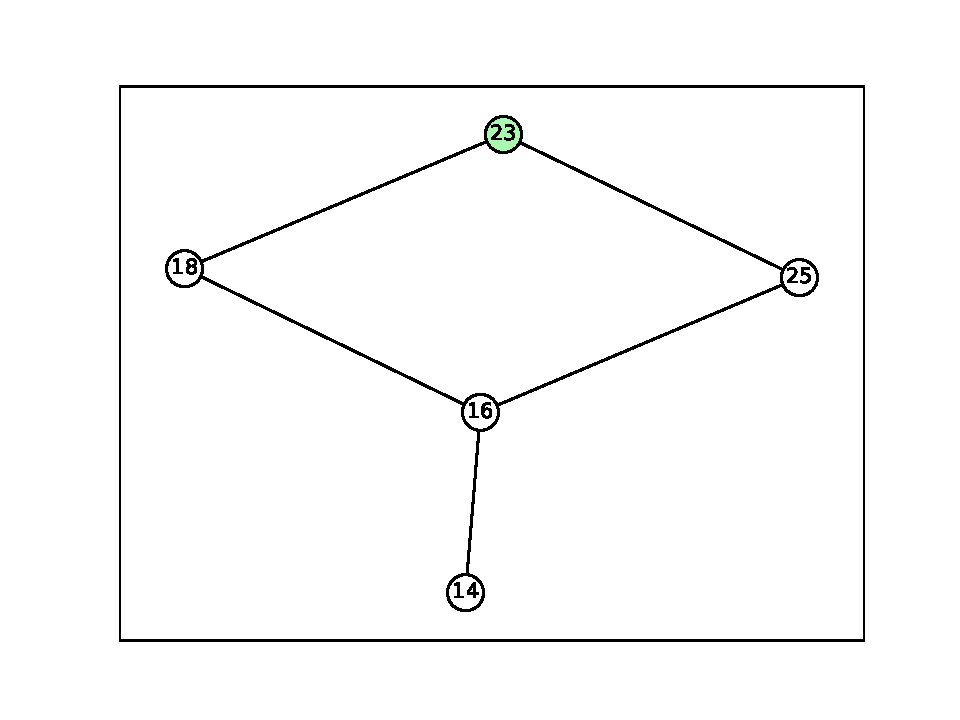
\includegraphics[width=0.5\textwidth]{task11-graphlets/5_14-16-18-25-23.pdf} &
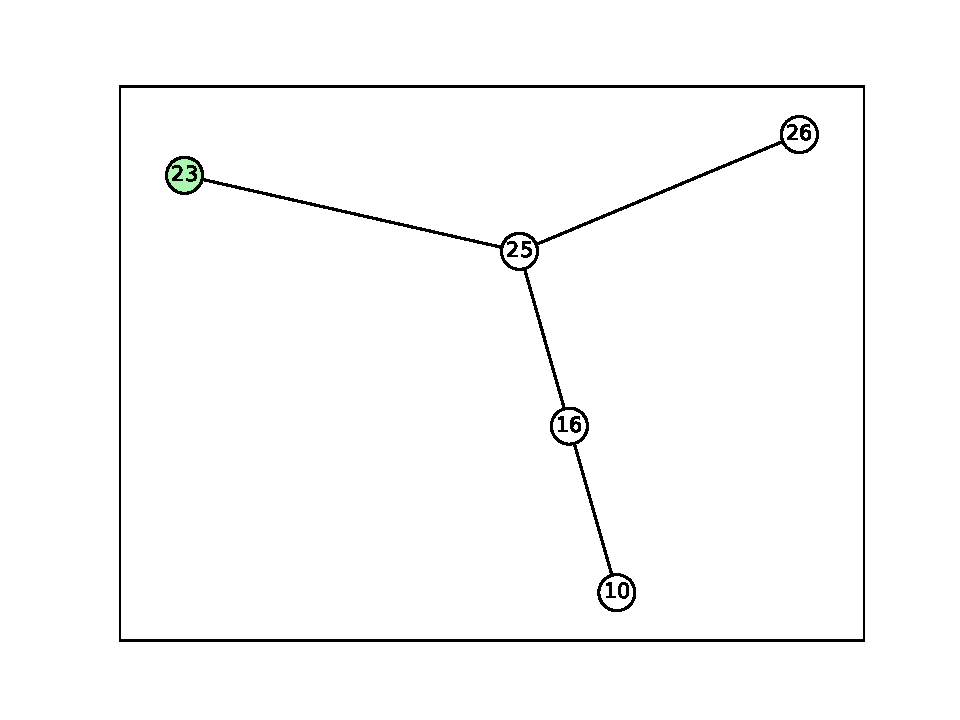
\includegraphics[width=0.5\textwidth]{task11-graphlets/5_10-16-25-23-26.pdf} \\
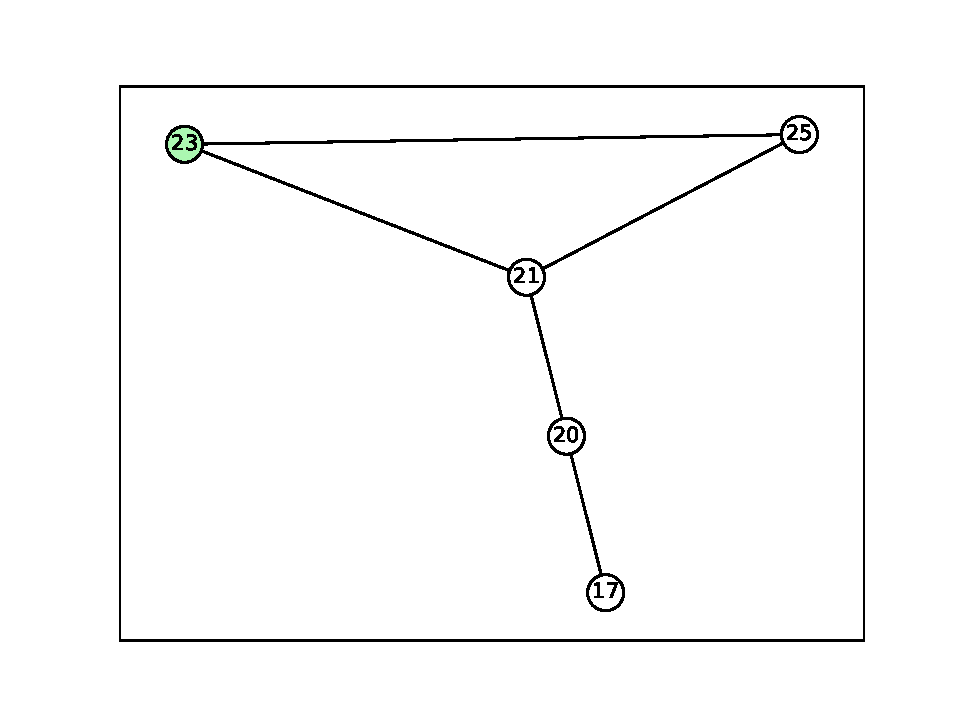
\includegraphics[width=0.5\textwidth]{task11-graphlets/5_21-17-25-20-23.pdf} &
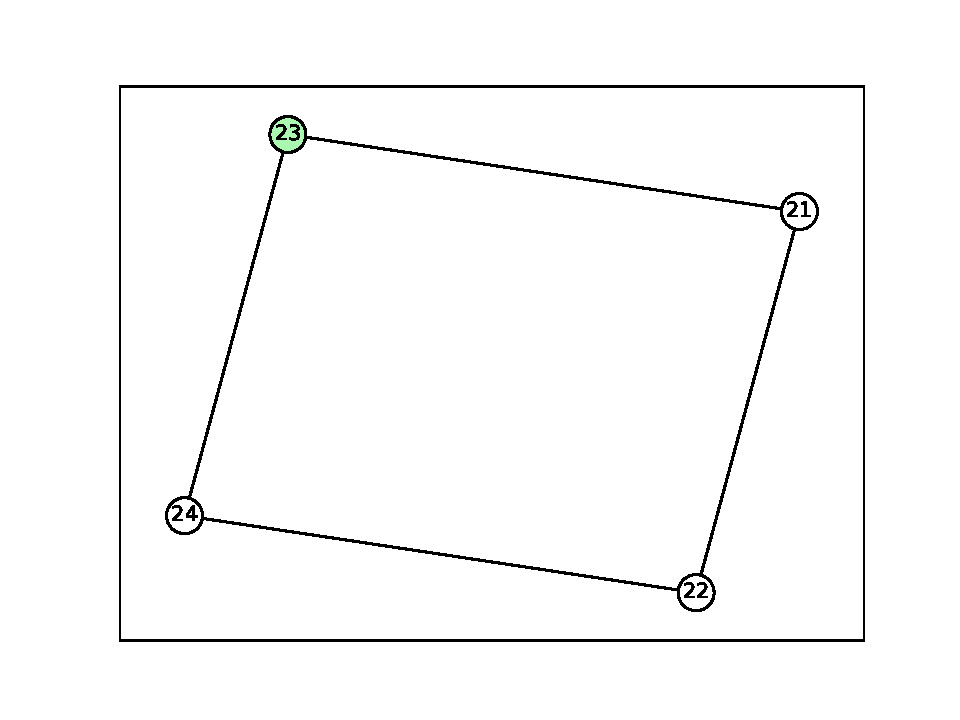
\includegraphics[width=0.5\textwidth]{task11-graphlets/4_21-22-23-24.pdf} \\
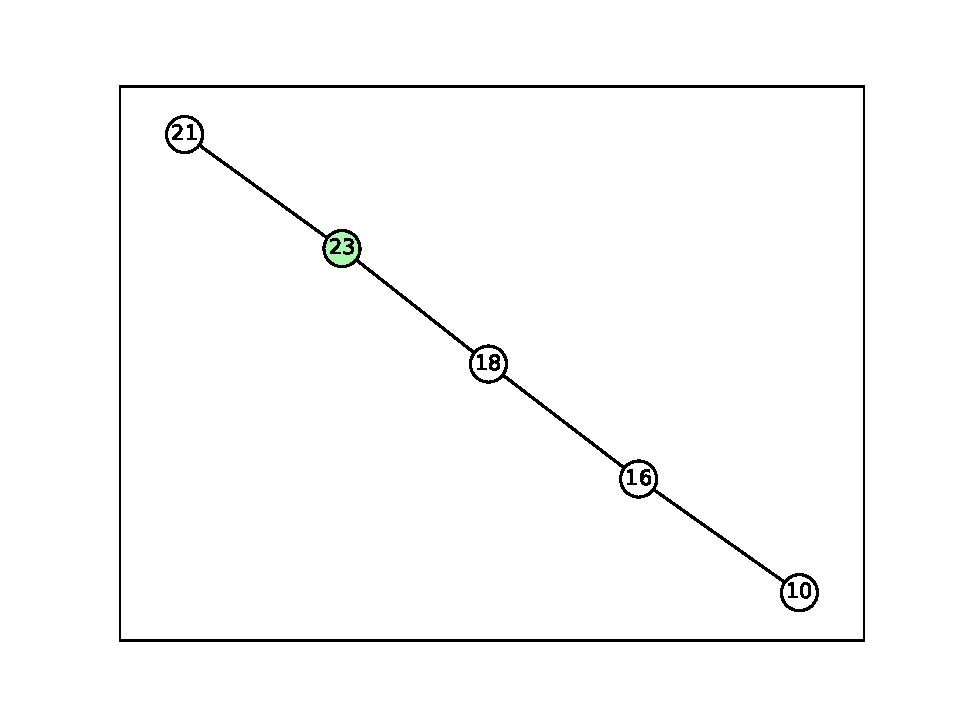
\includegraphics[width=0.5\textwidth]{task11-graphlets/5_10-16-21-18-23.pdf} &
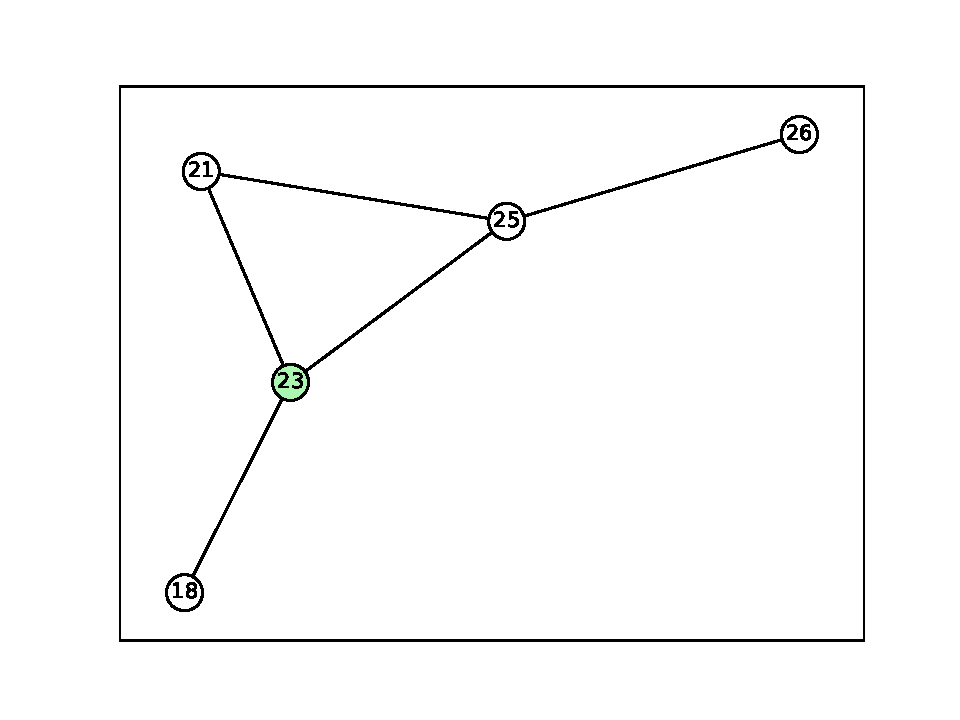
\includegraphics[width=0.5\textwidth]{task11-graphlets/5_21-18-25-23-26.pdf} \\
\end{tabularx}\end{figure}
\begin{figure}\centering\begin{tabularx}{\textwidth}{cc}
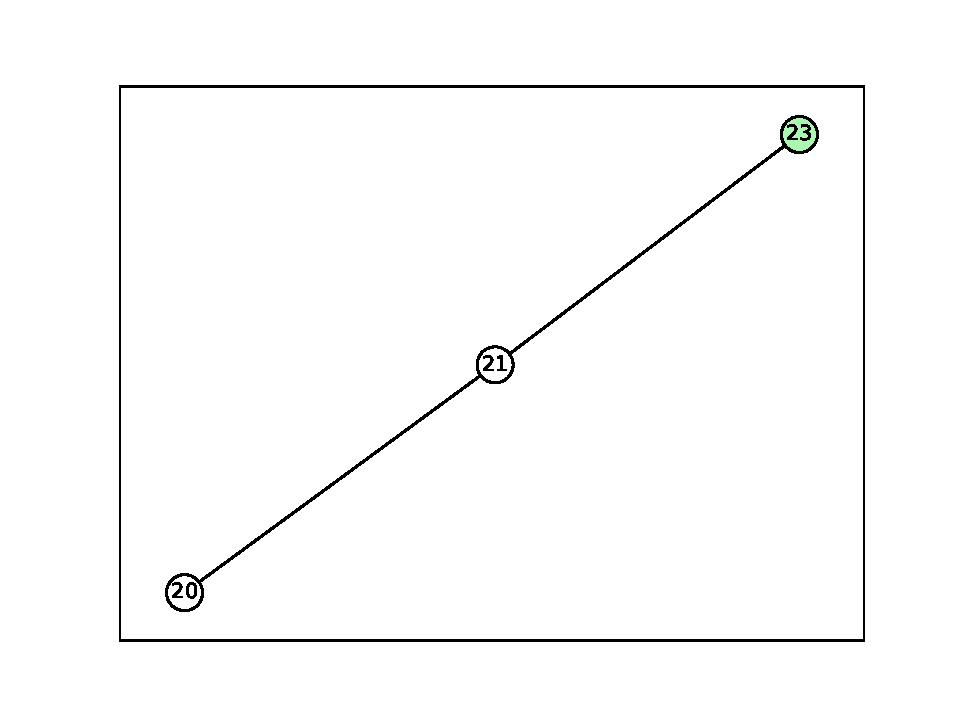
\includegraphics[width=0.5\textwidth]{task11-graphlets/3_21-20-23.pdf} &
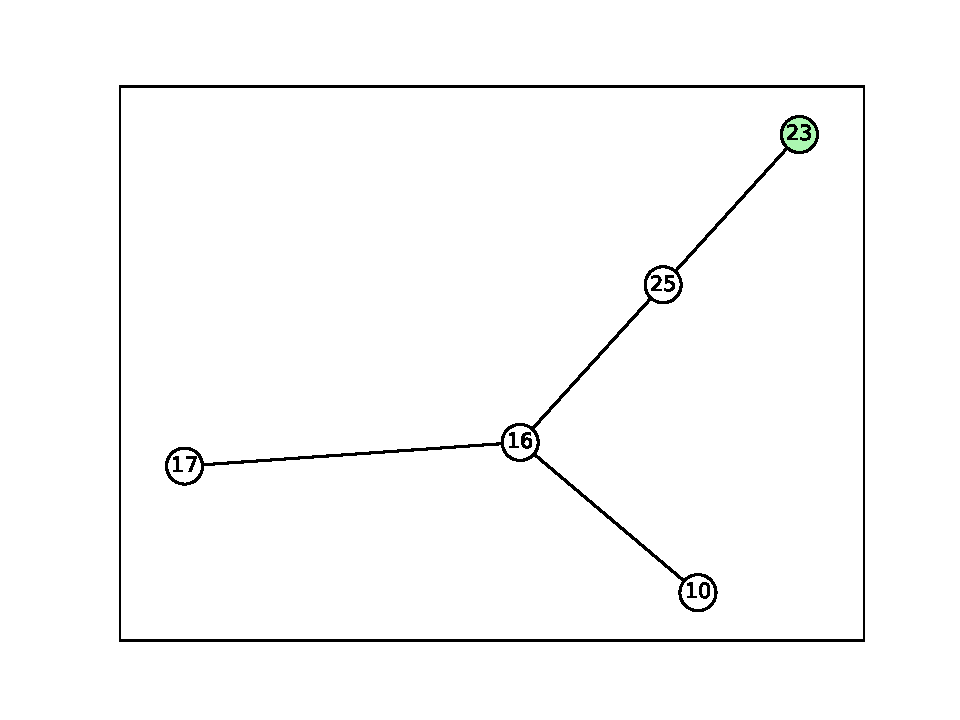
\includegraphics[width=0.5\textwidth]{task11-graphlets/5_10-16-17-25-23.pdf} \\
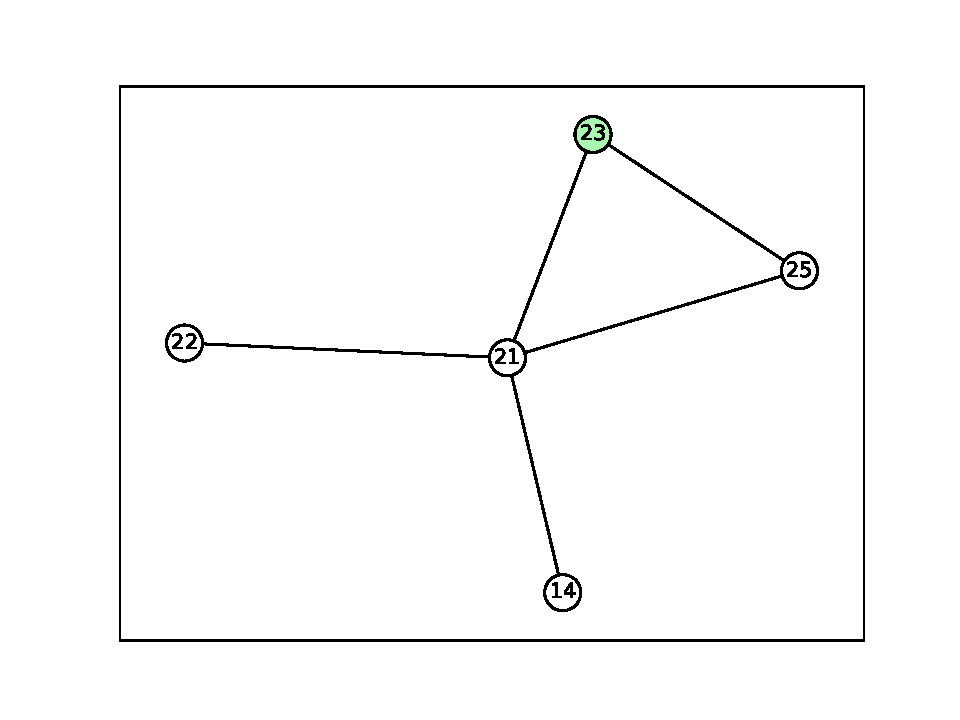
\includegraphics[width=0.5\textwidth]{task11-graphlets/5_14-21-25-22-23.pdf} &
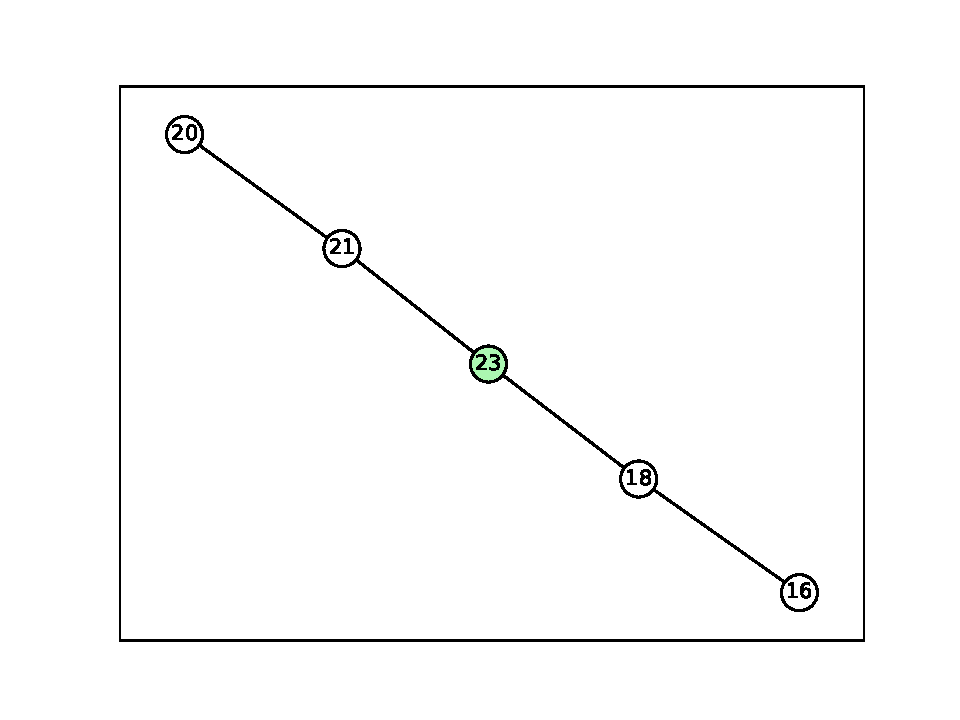
\includegraphics[width=0.5\textwidth]{task11-graphlets/5_16-21-18-20-23.pdf} \\
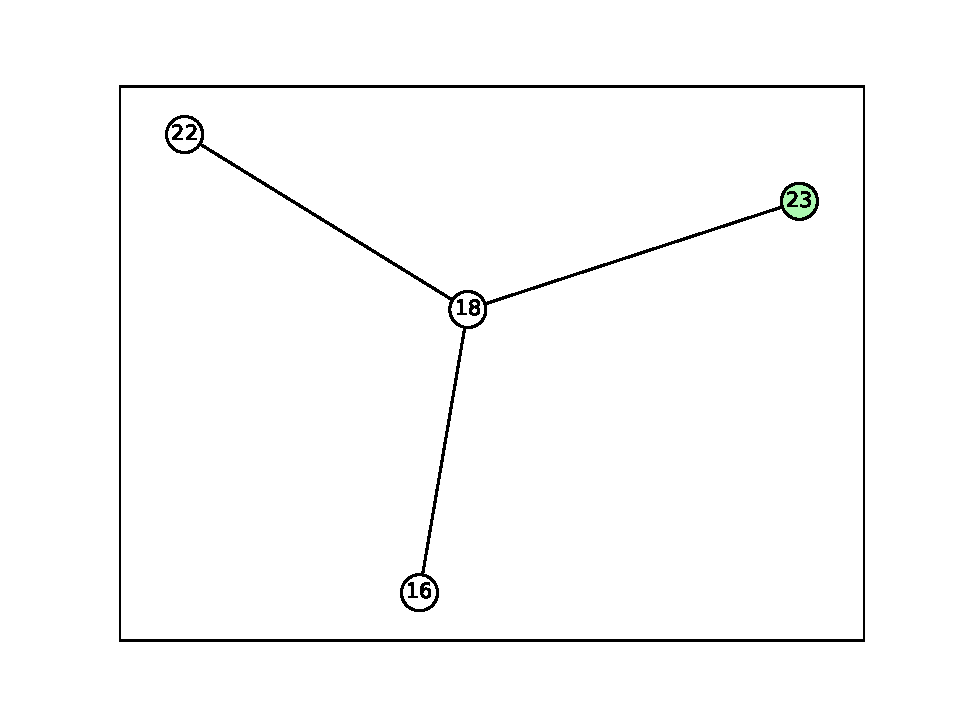
\includegraphics[width=0.5\textwidth]{task11-graphlets/4_16-18-22-23.pdf} &
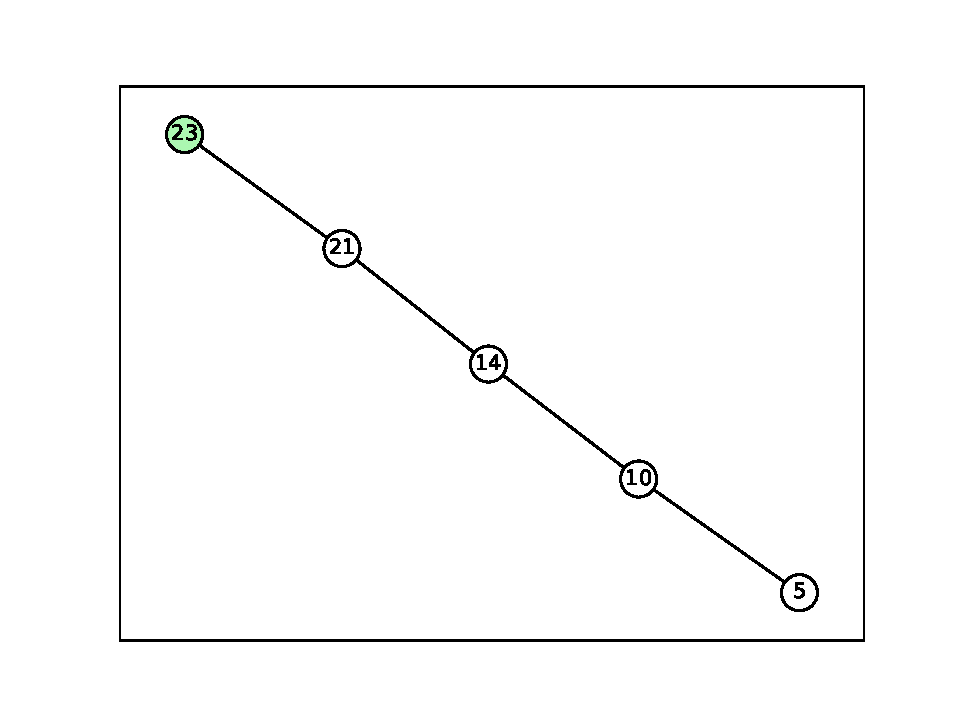
\includegraphics[width=0.5\textwidth]{task11-graphlets/5_5-10-14-21-23.pdf} \\
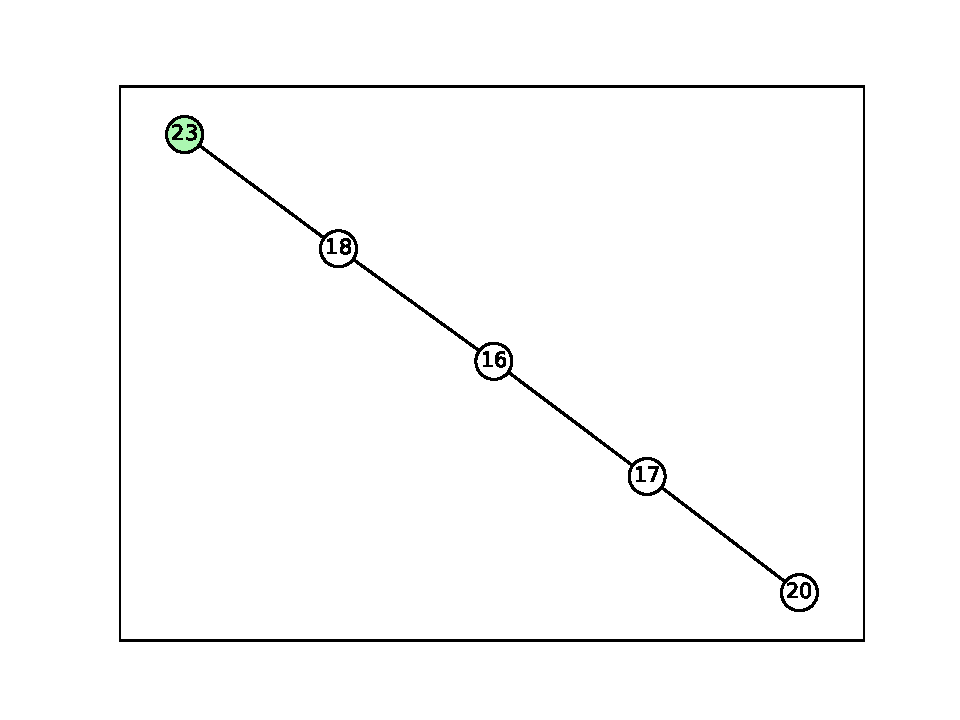
\includegraphics[width=0.5\textwidth]{task11-graphlets/5_16-17-18-20-23.pdf} &
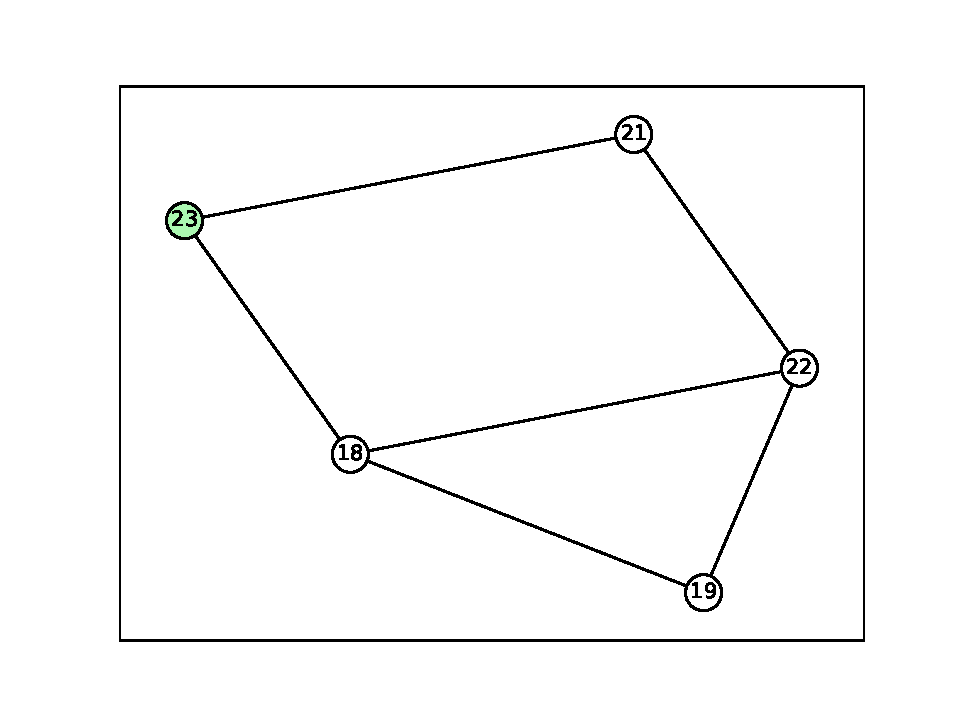
\includegraphics[width=0.5\textwidth]{task11-graphlets/5_21-18-19-22-23.pdf} \\
\end{tabularx}\end{figure}
\begin{figure}\centering\begin{tabularx}{\textwidth}{cc}
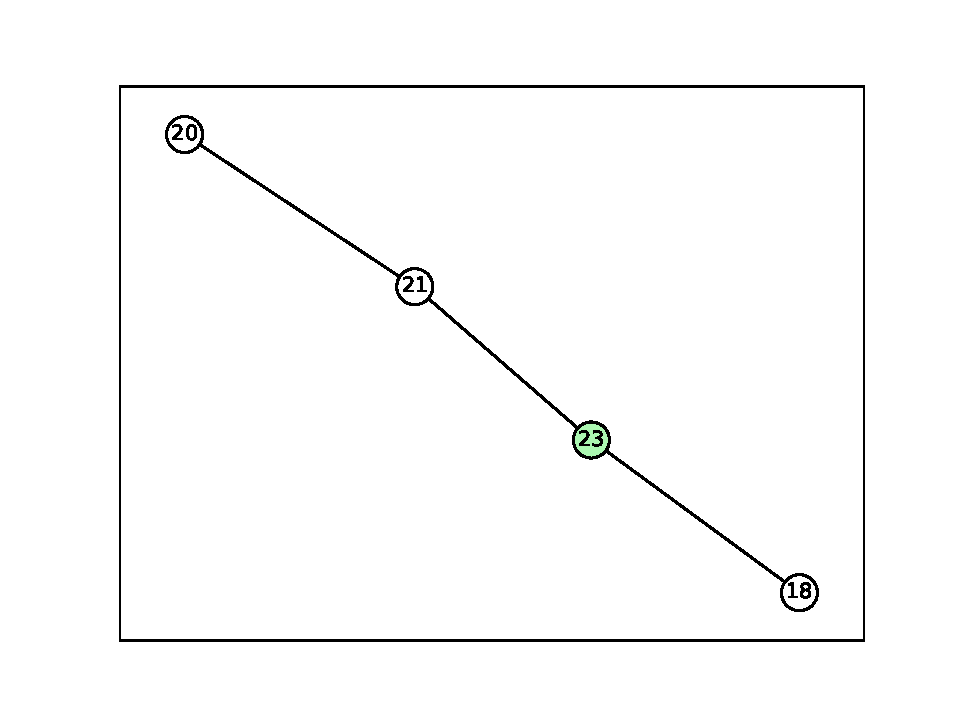
\includegraphics[width=0.5\textwidth]{task11-graphlets/4_21-18-20-23.pdf} &
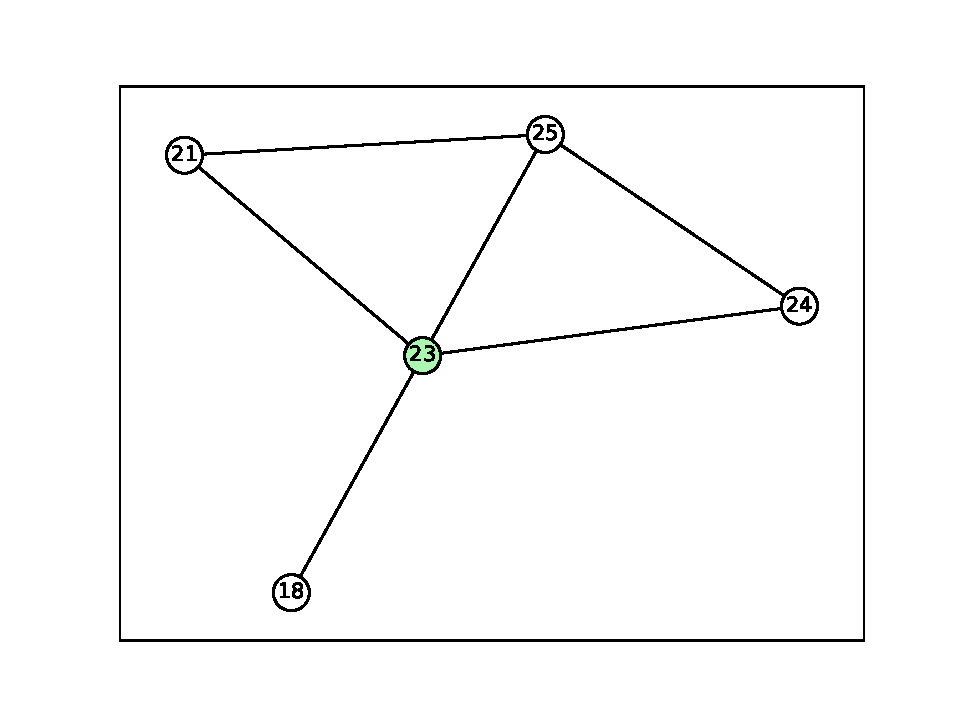
\includegraphics[width=0.5\textwidth]{task11-graphlets/5_21-18-25-23-24.pdf} \\
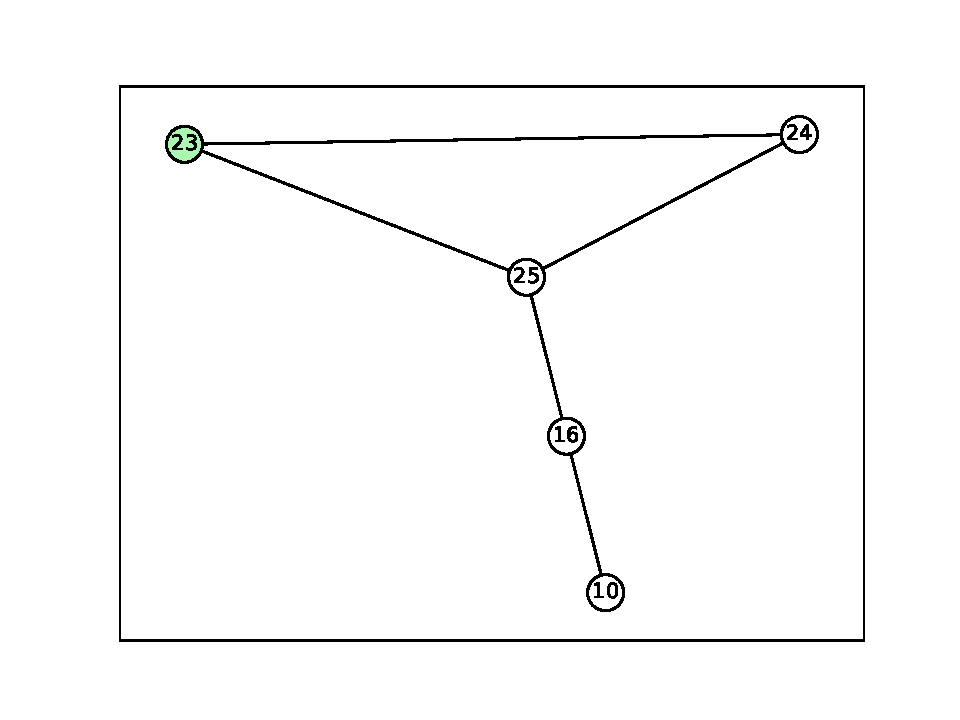
\includegraphics[width=0.5\textwidth]{task11-graphlets/5_10-16-25-23-24.pdf} &
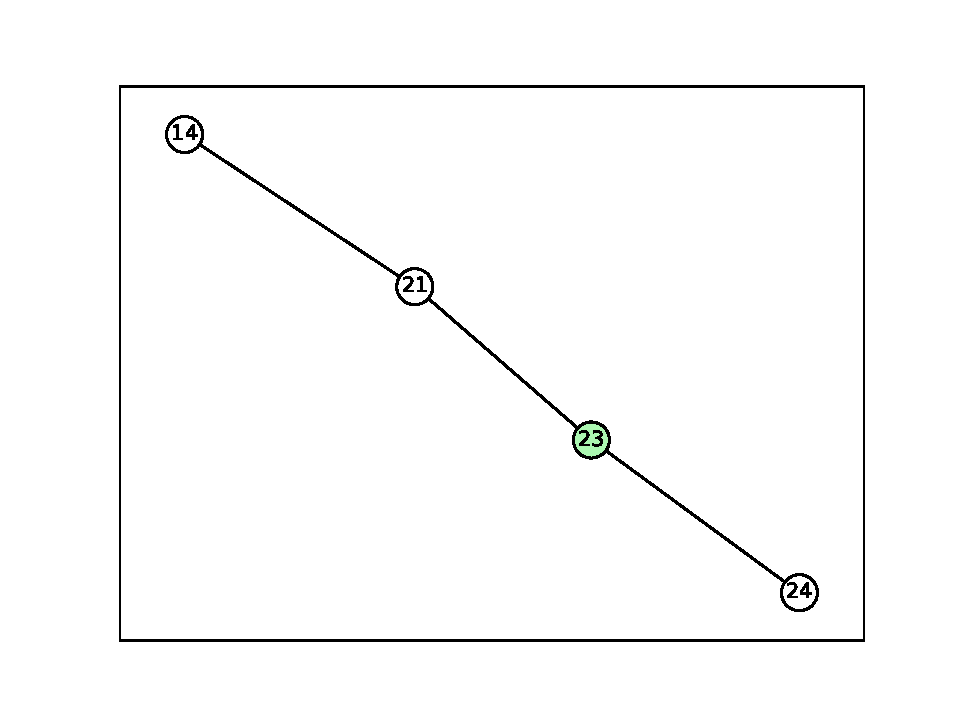
\includegraphics[width=0.5\textwidth]{task11-graphlets/4_14-21-23-24.pdf} \\
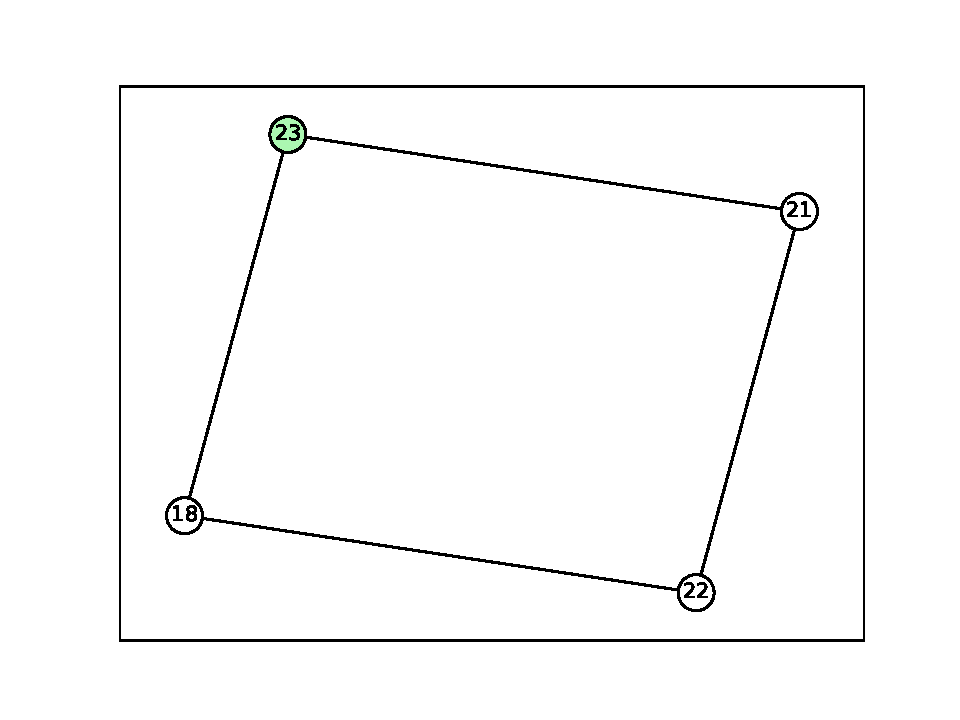
\includegraphics[width=0.5\textwidth]{task11-graphlets/4_21-18-22-23.pdf} &
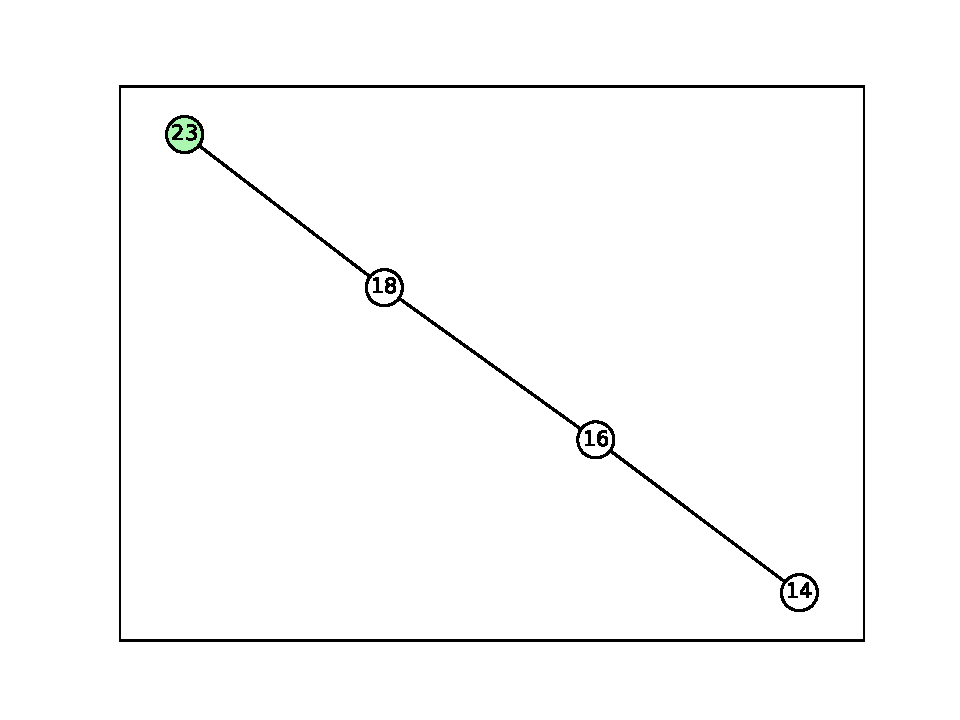
\includegraphics[width=0.5\textwidth]{task11-graphlets/4_14-16-18-23.pdf} \\
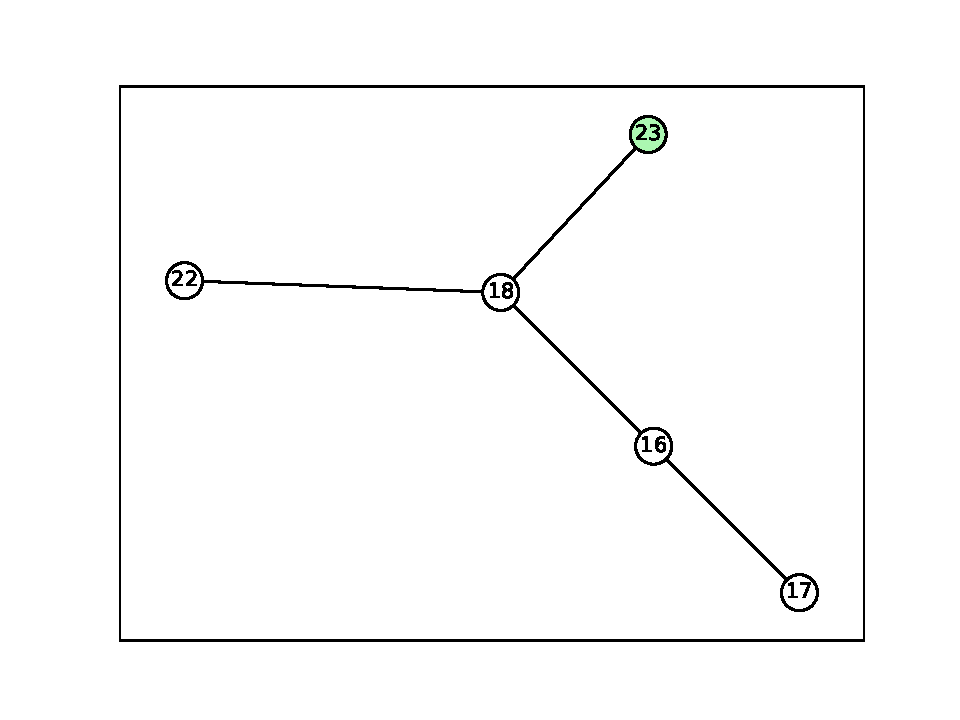
\includegraphics[width=0.5\textwidth]{task11-graphlets/5_16-17-18-22-23.pdf} &
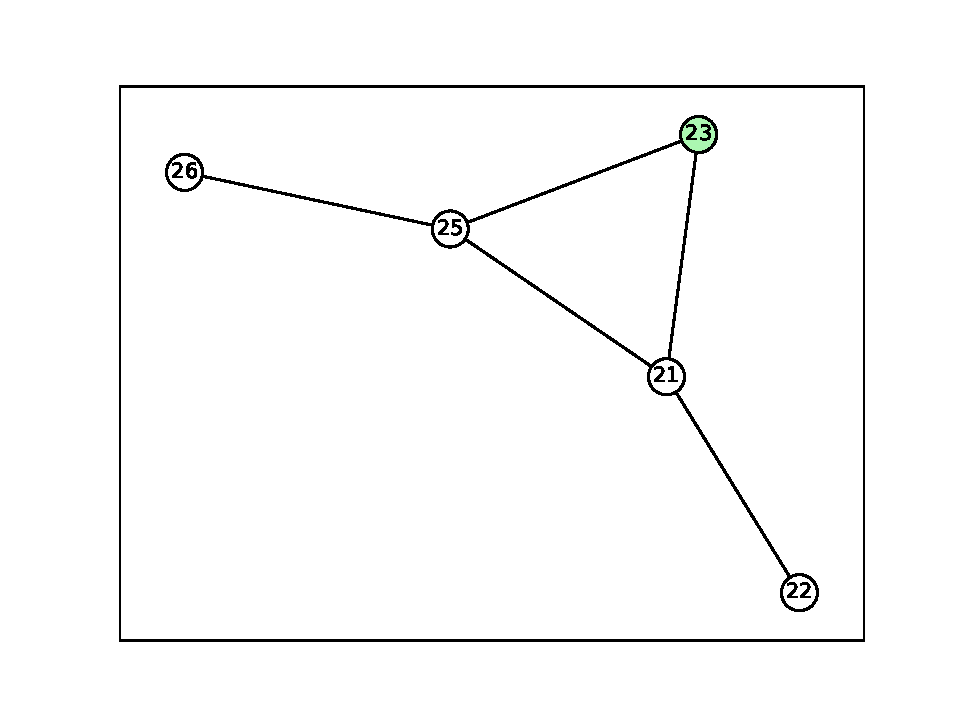
\includegraphics[width=0.5\textwidth]{task11-graphlets/5_21-25-22-23-26.pdf} \\
\end{tabularx}\end{figure}
\begin{figure}\centering\begin{tabularx}{\textwidth}{cc}
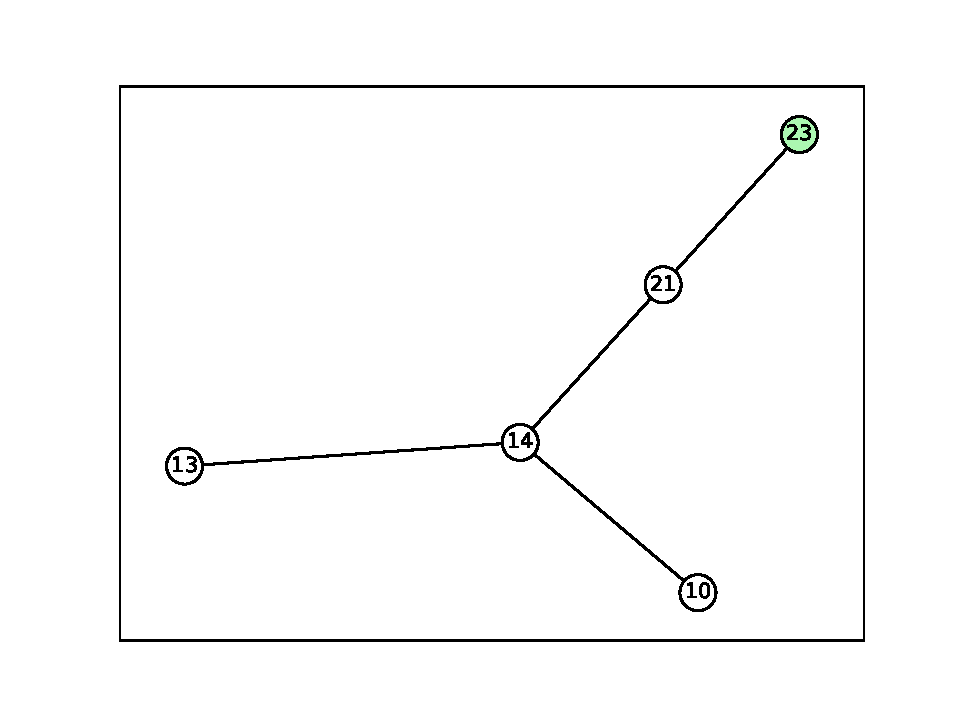
\includegraphics[width=0.5\textwidth]{task11-graphlets/5_10-14-13-21-23.pdf} &
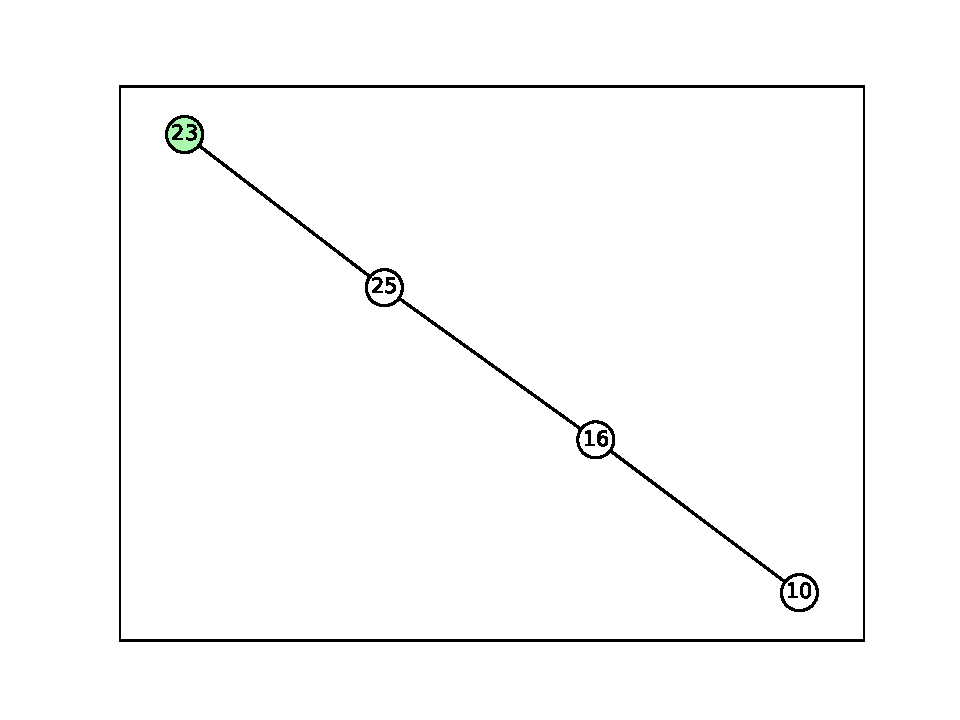
\includegraphics[width=0.5\textwidth]{task11-graphlets/4_10-16-25-23.pdf} \\
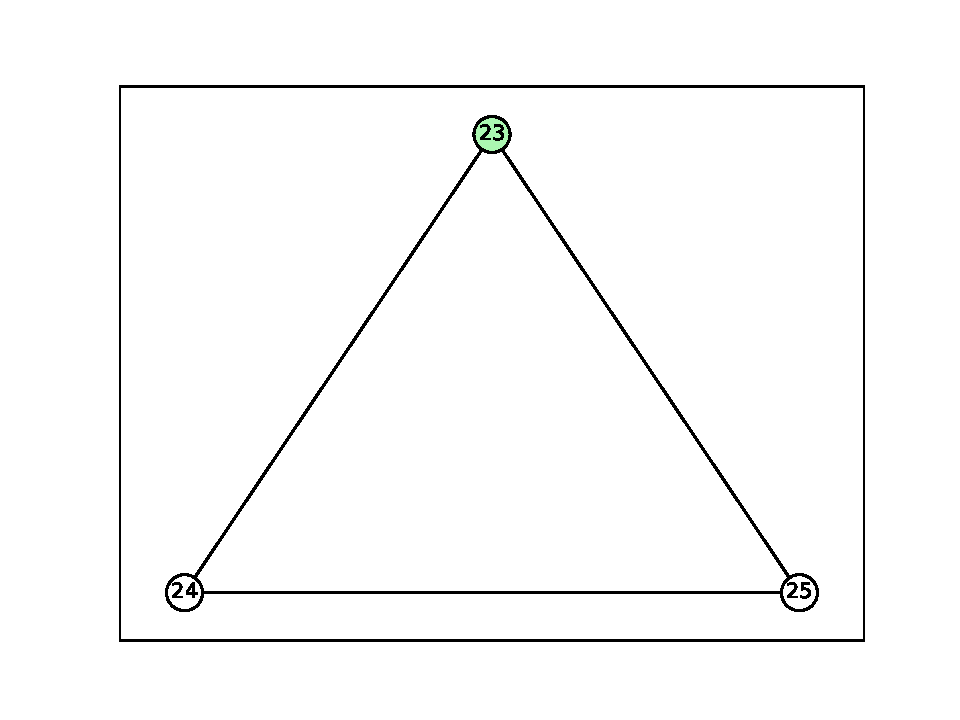
\includegraphics[width=0.5\textwidth]{task11-graphlets/3_25-23-24.pdf} &
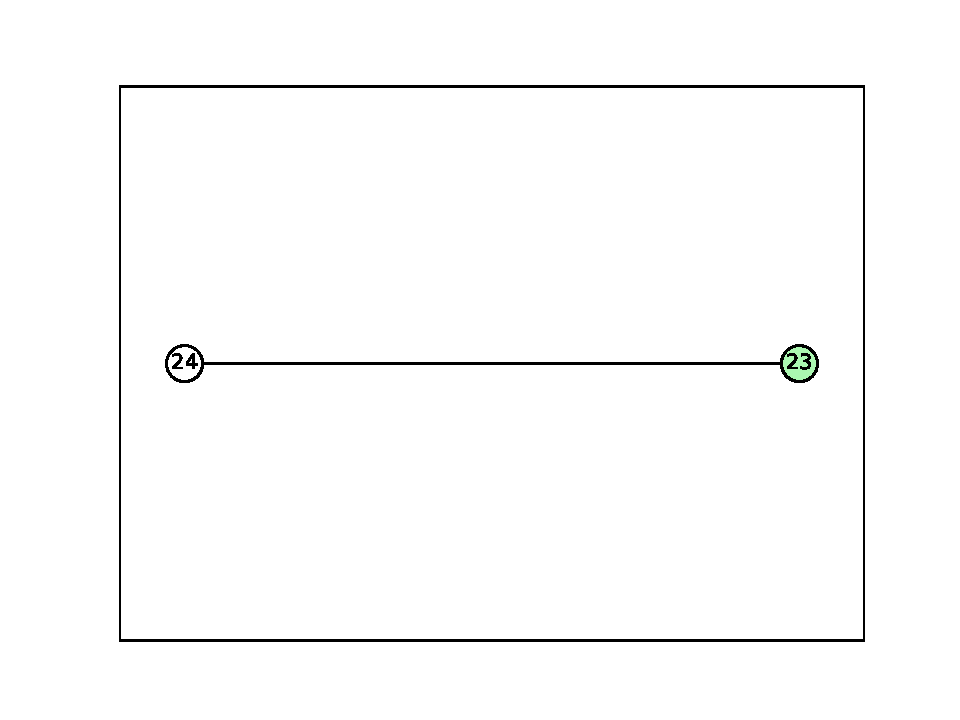
\includegraphics[width=0.5\textwidth]{task11-graphlets/2_23-24.pdf} \\
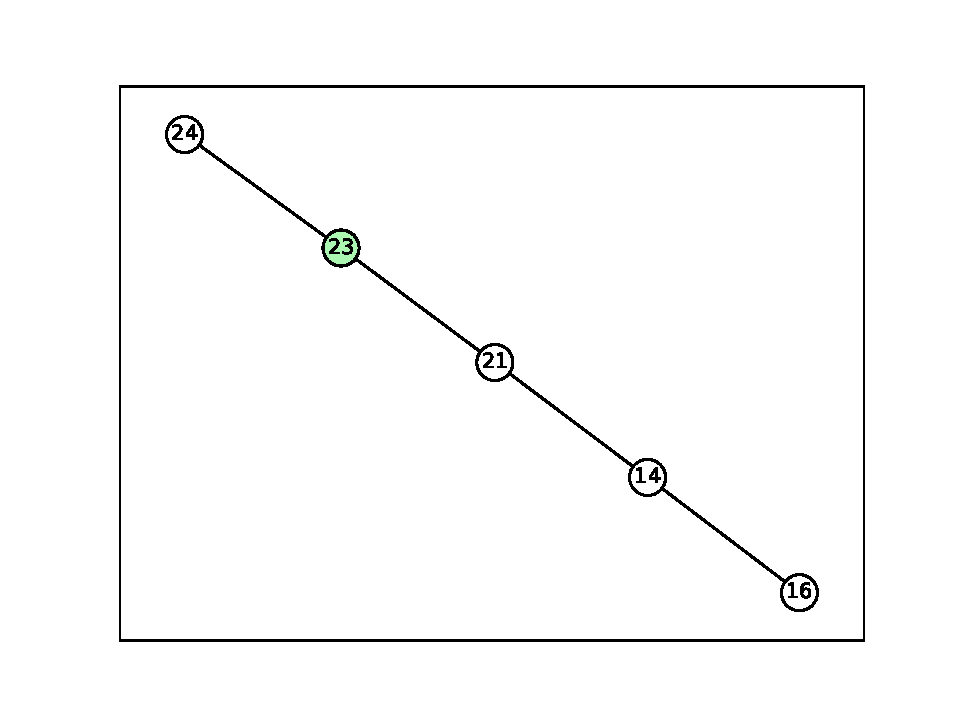
\includegraphics[width=0.5\textwidth]{task11-graphlets/5_14-16-21-23-24.pdf} &
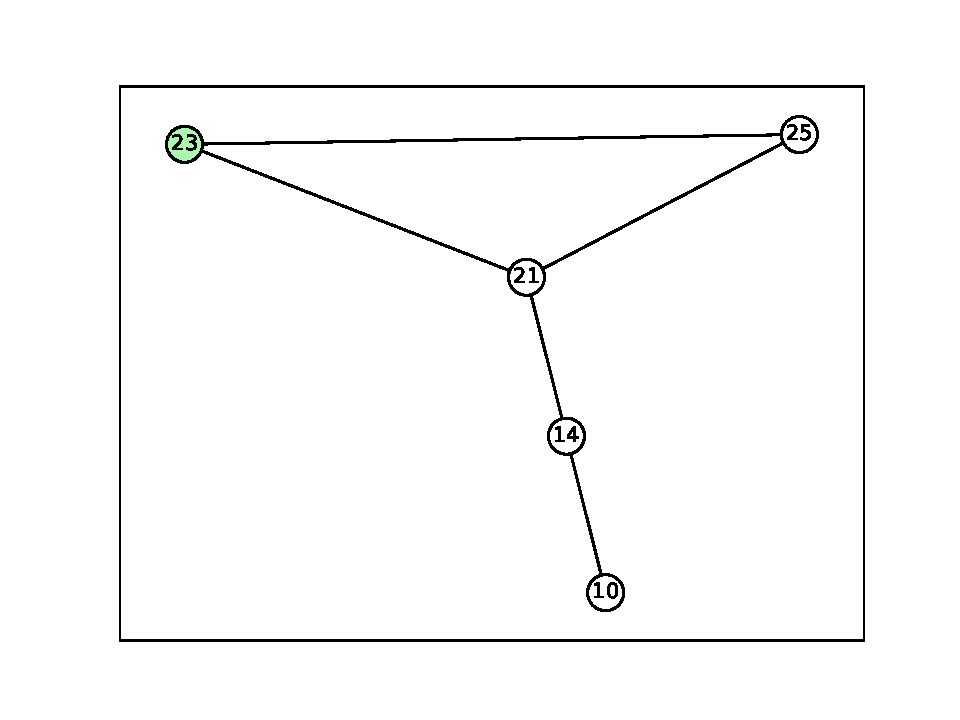
\includegraphics[width=0.5\textwidth]{task11-graphlets/5_10-14-21-25-23.pdf} \\
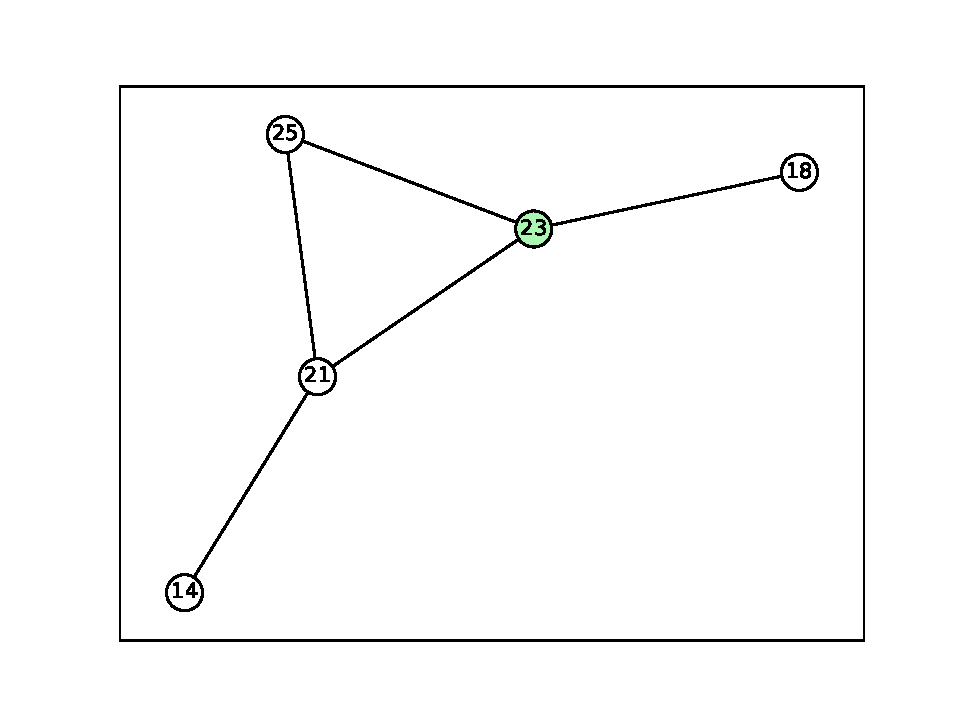
\includegraphics[width=0.5\textwidth]{task11-graphlets/5_14-21-18-25-23.pdf} &
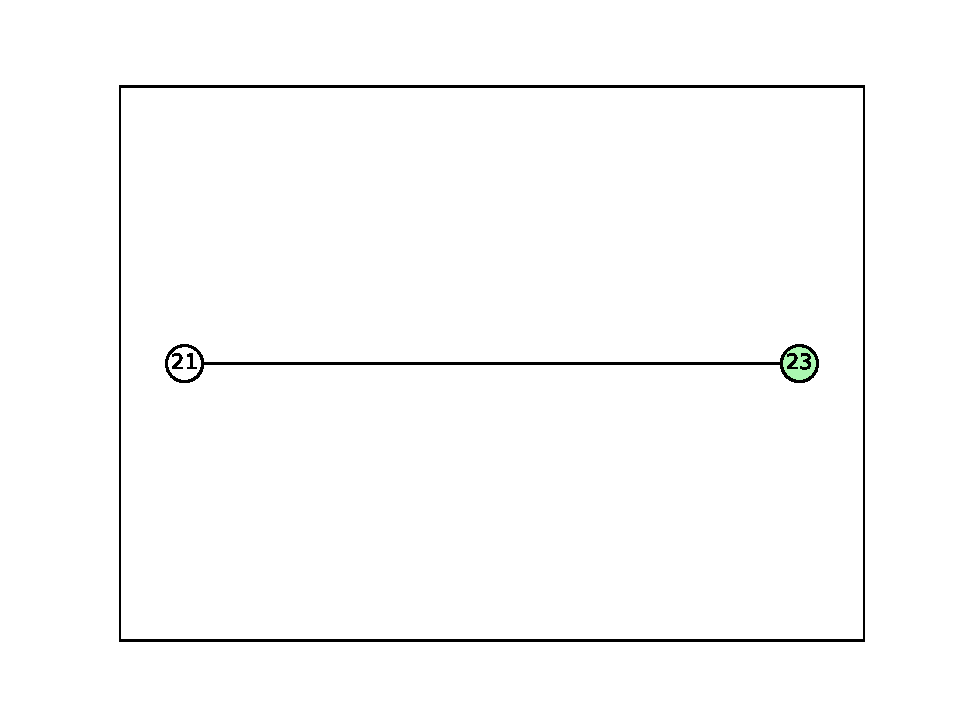
\includegraphics[width=0.5\textwidth]{task11-graphlets/2_21-23.pdf} \\
\end{tabularx}\end{figure}
\begin{figure}\centering\begin{tabularx}{\textwidth}{cc}
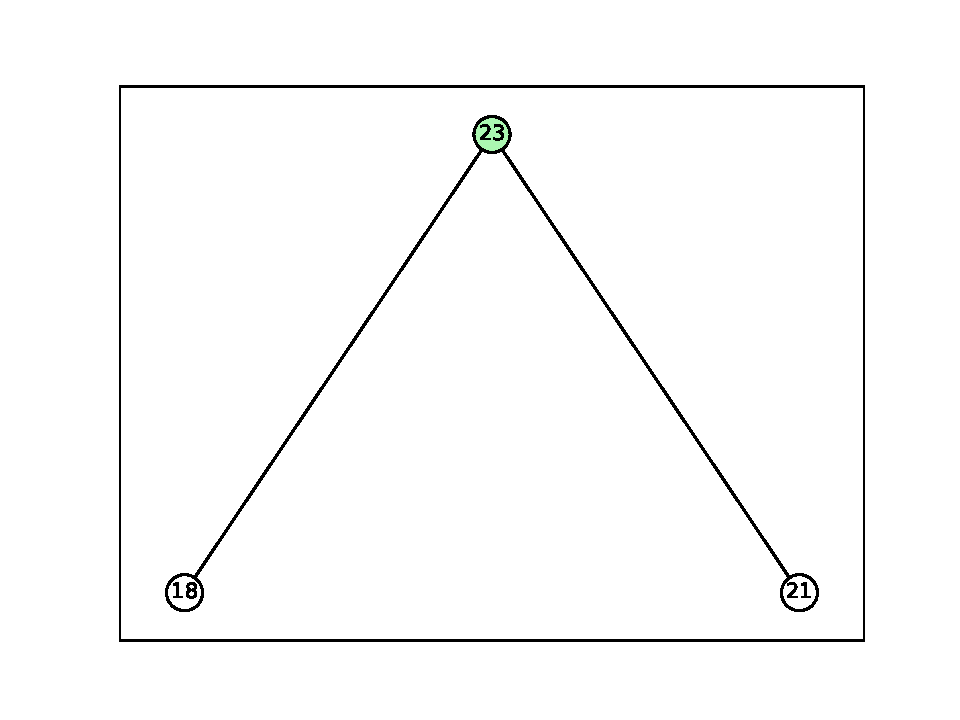
\includegraphics[width=0.5\textwidth]{task11-graphlets/3_21-18-23.pdf} &
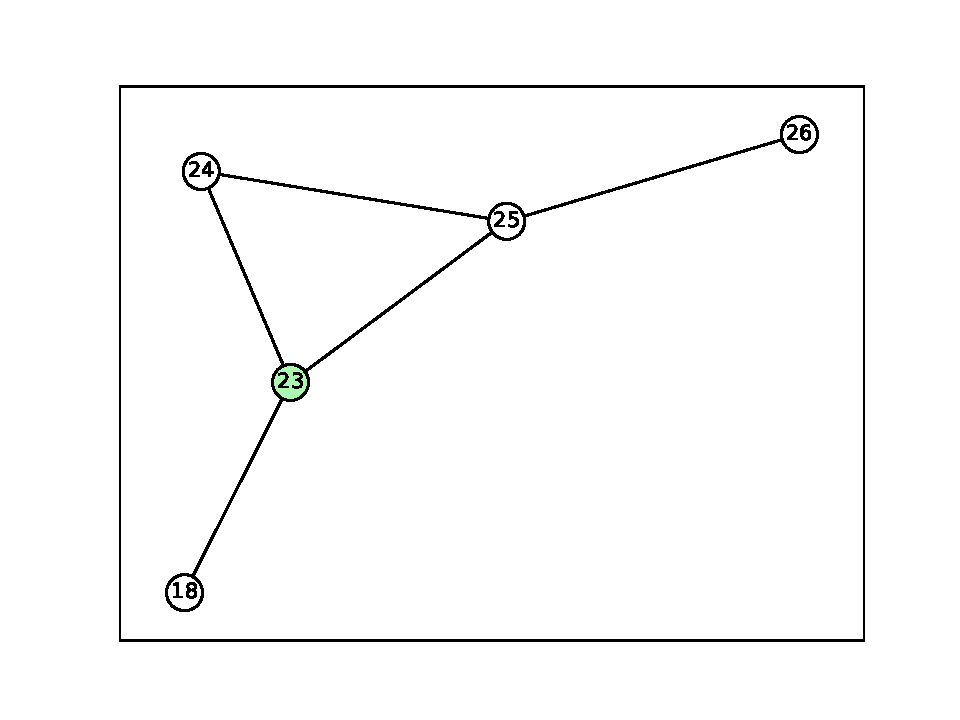
\includegraphics[width=0.5\textwidth]{task11-graphlets/5_18-25-23-24-26.pdf} \\
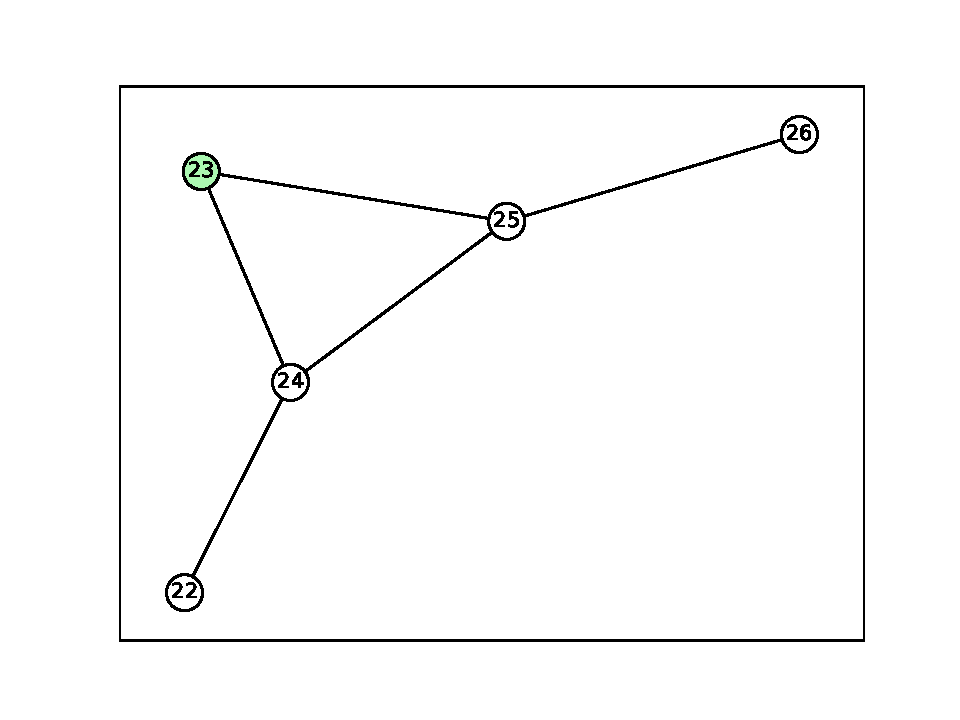
\includegraphics[width=0.5\textwidth]{task11-graphlets/5_25-22-23-24-26.pdf} &
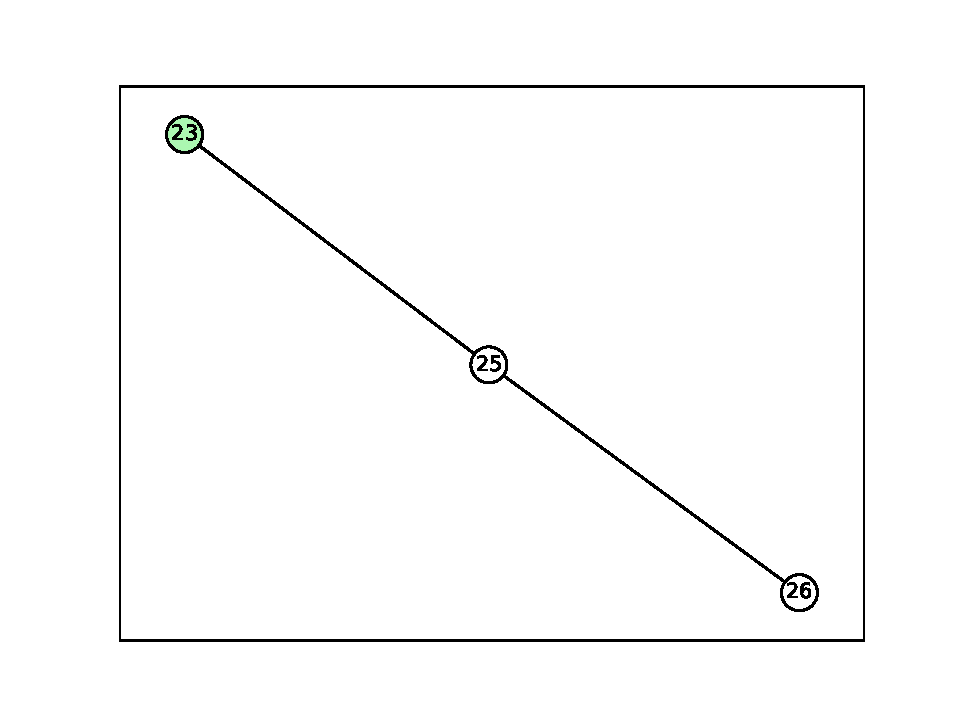
\includegraphics[width=0.5\textwidth]{task11-graphlets/3_25-23-26.pdf} \\
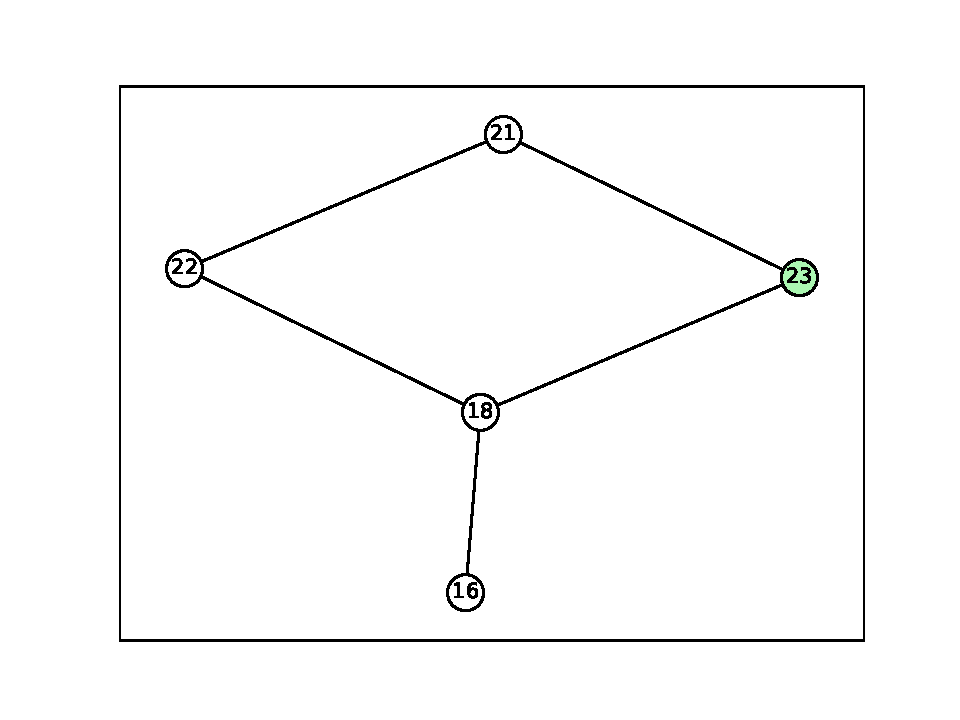
\includegraphics[width=0.5\textwidth]{task11-graphlets/5_16-21-18-22-23.pdf} &
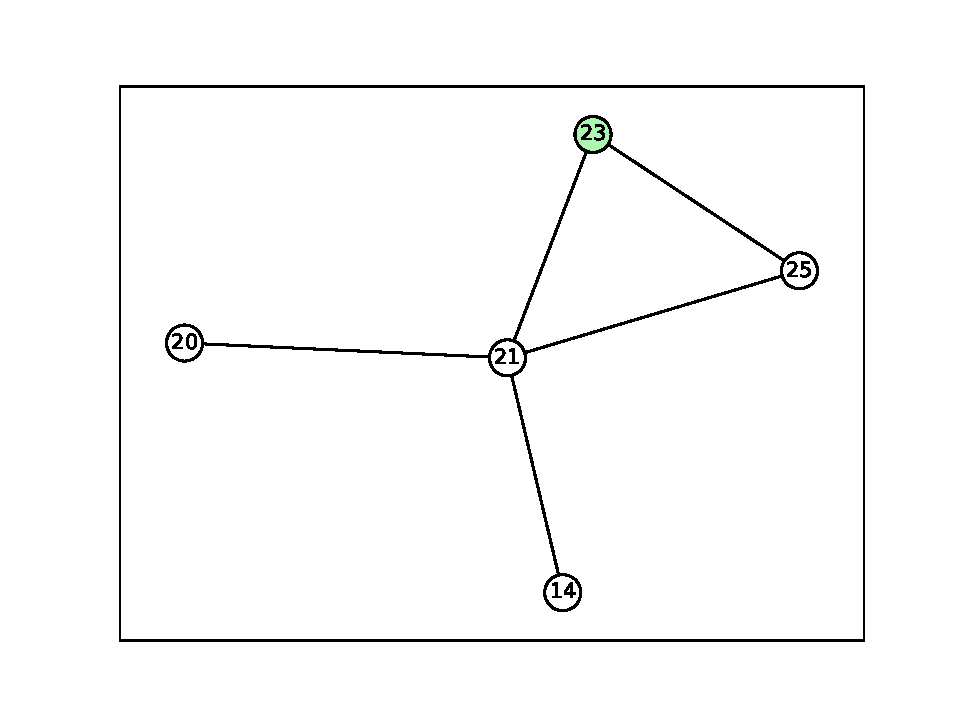
\includegraphics[width=0.5\textwidth]{task11-graphlets/5_14-21-25-20-23.pdf} \\
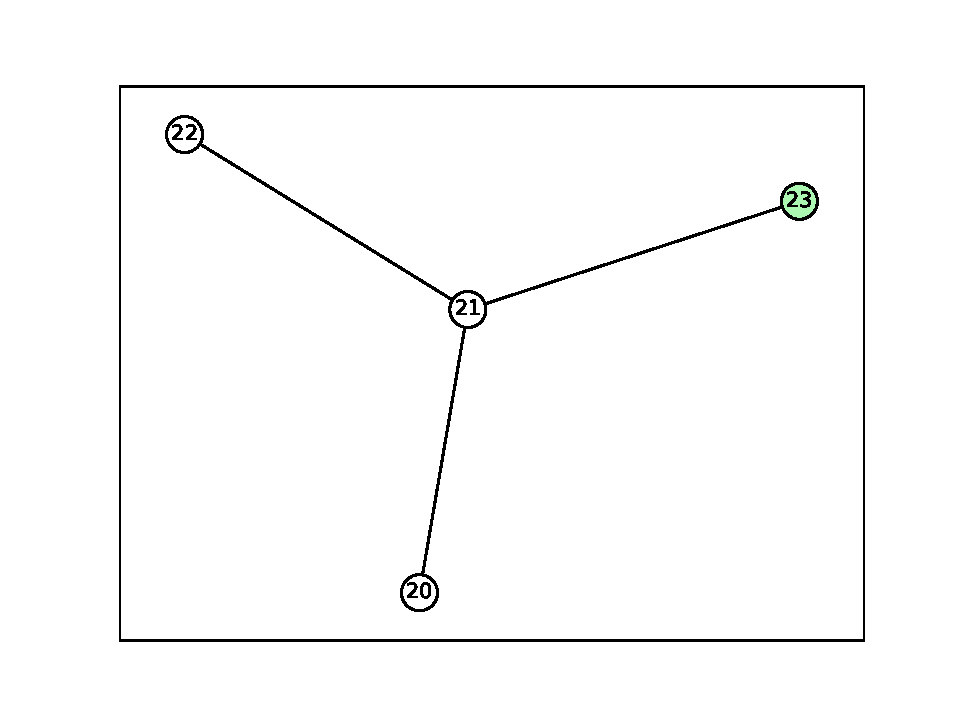
\includegraphics[width=0.5\textwidth]{task11-graphlets/4_21-20-22-23.pdf} &
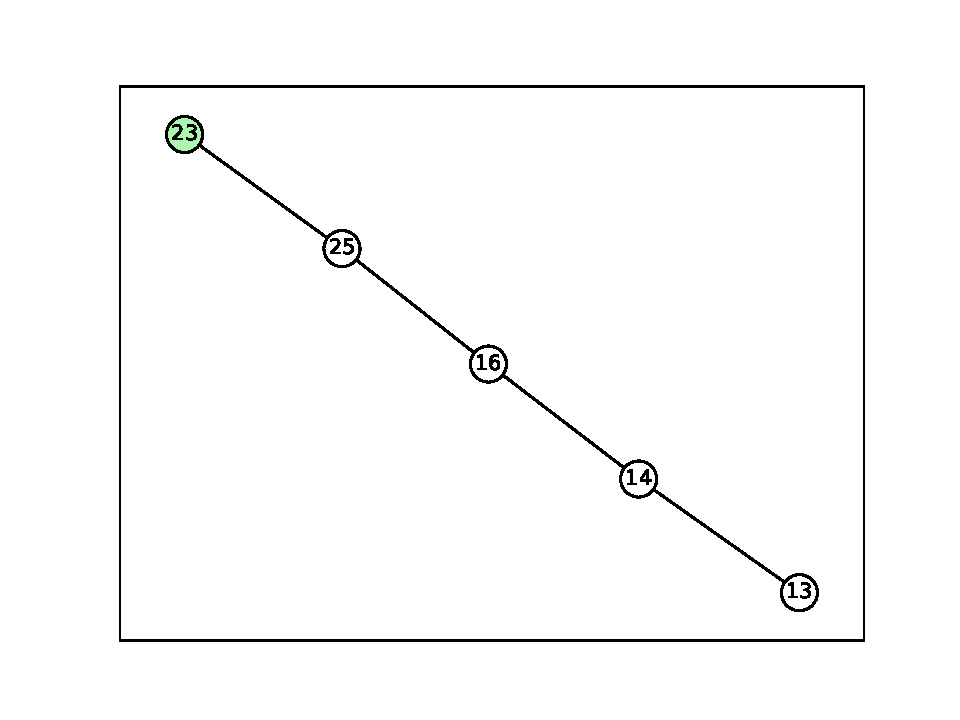
\includegraphics[width=0.5\textwidth]{task11-graphlets/5_14-16-13-25-23.pdf} \\
\end{tabularx}\end{figure}
\begin{figure}\centering\begin{tabularx}{\textwidth}{cc}
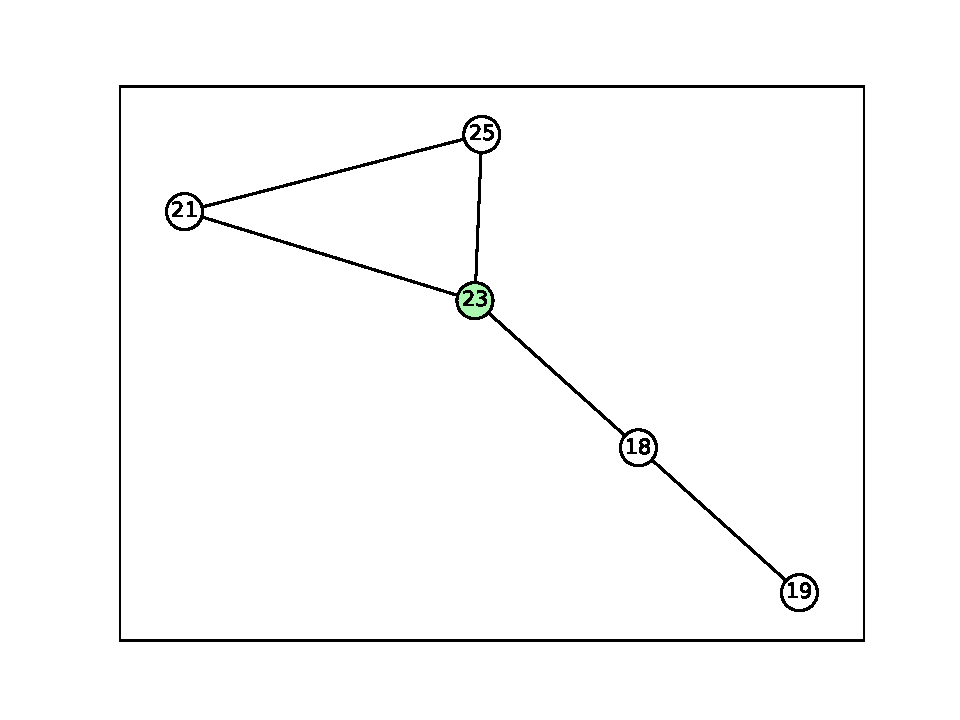
\includegraphics[width=0.5\textwidth]{task11-graphlets/5_21-18-25-19-23.pdf} &
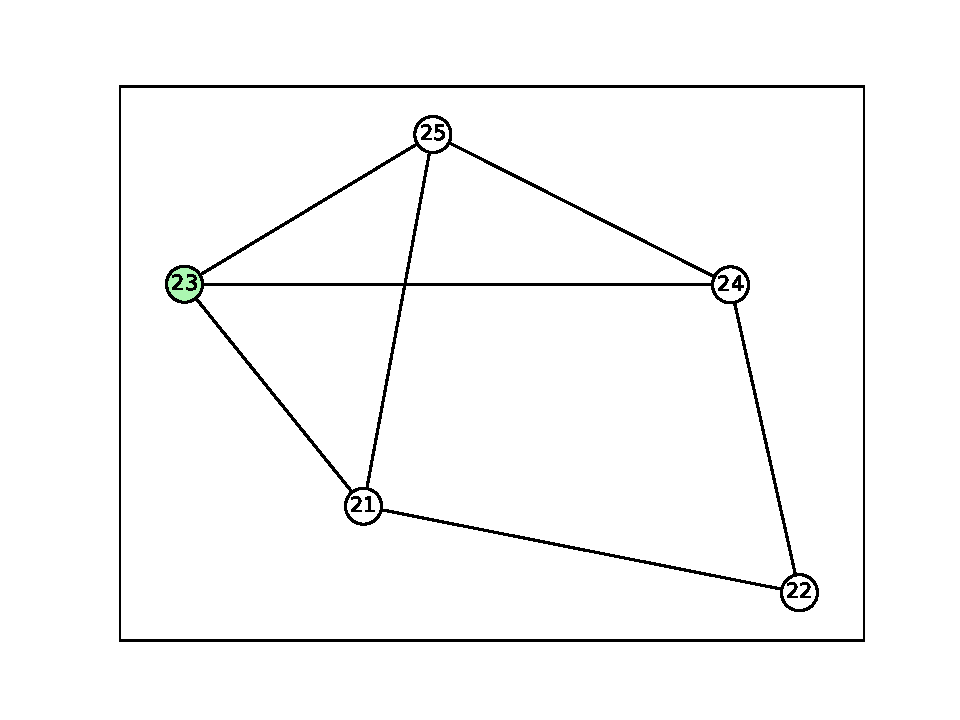
\includegraphics[width=0.5\textwidth]{task11-graphlets/5_21-25-22-23-24.pdf} \\
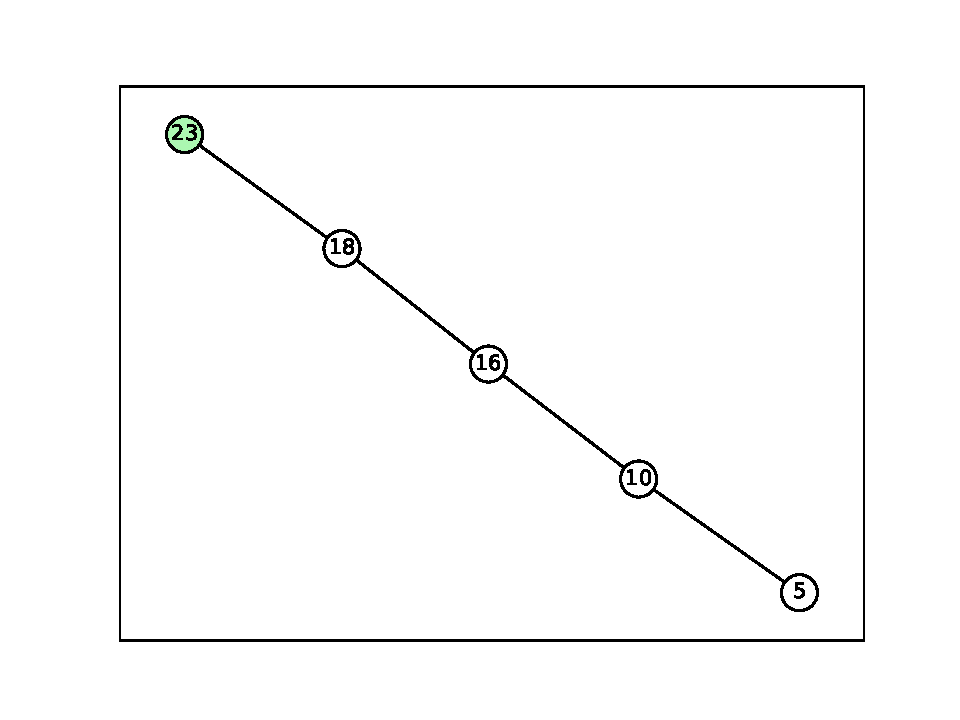
\includegraphics[width=0.5\textwidth]{task11-graphlets/5_5-10-16-18-23.pdf} &
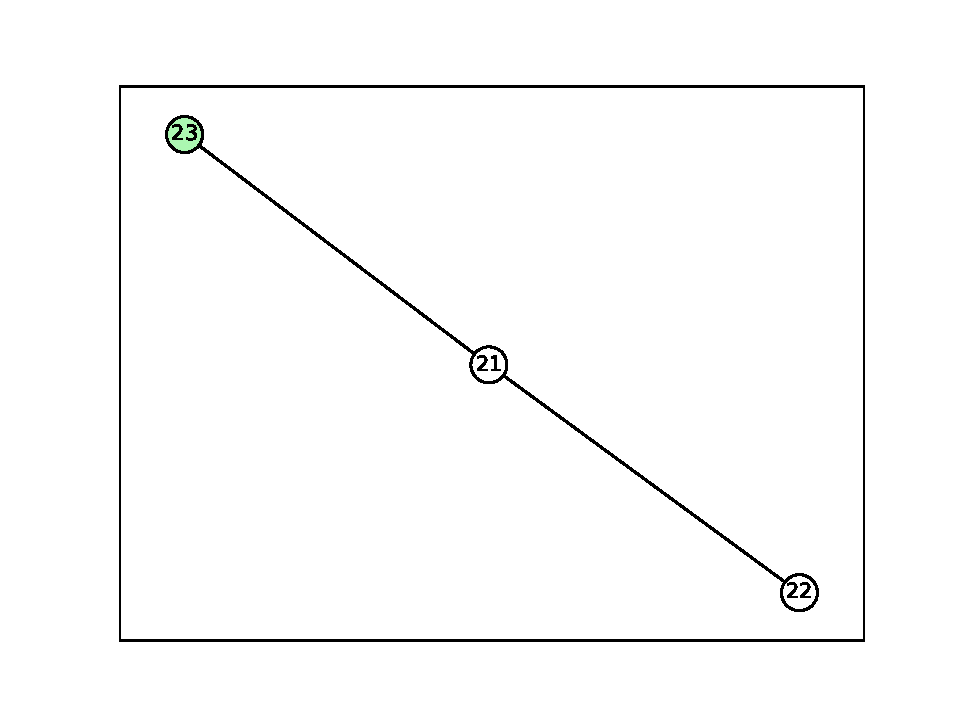
\includegraphics[width=0.5\textwidth]{task11-graphlets/3_21-22-23.pdf} \\
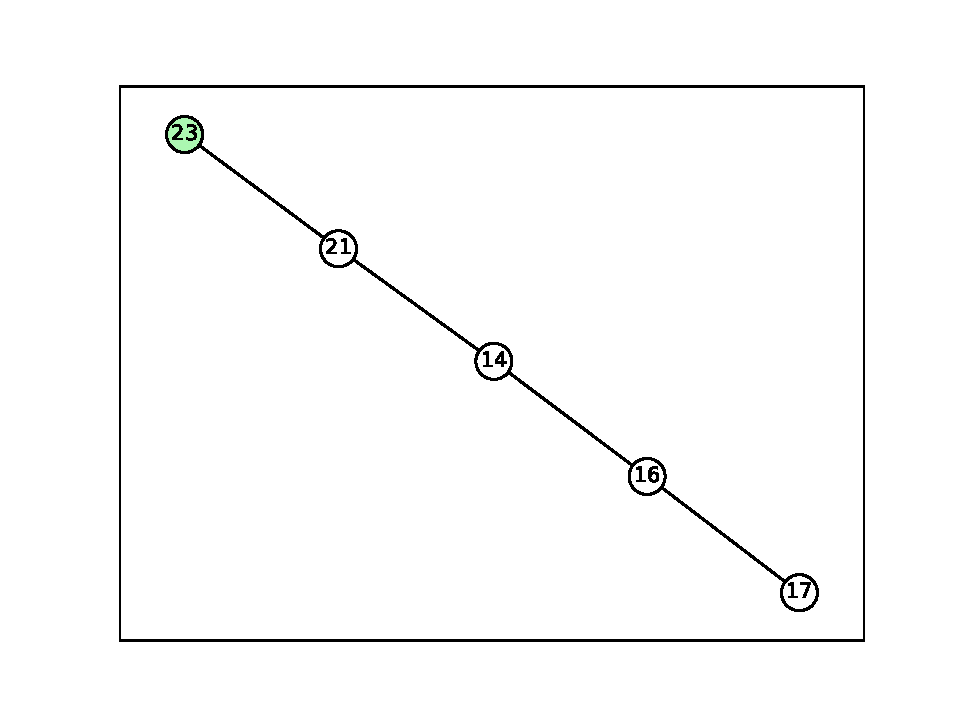
\includegraphics[width=0.5\textwidth]{task11-graphlets/5_14-16-21-17-23.pdf} &
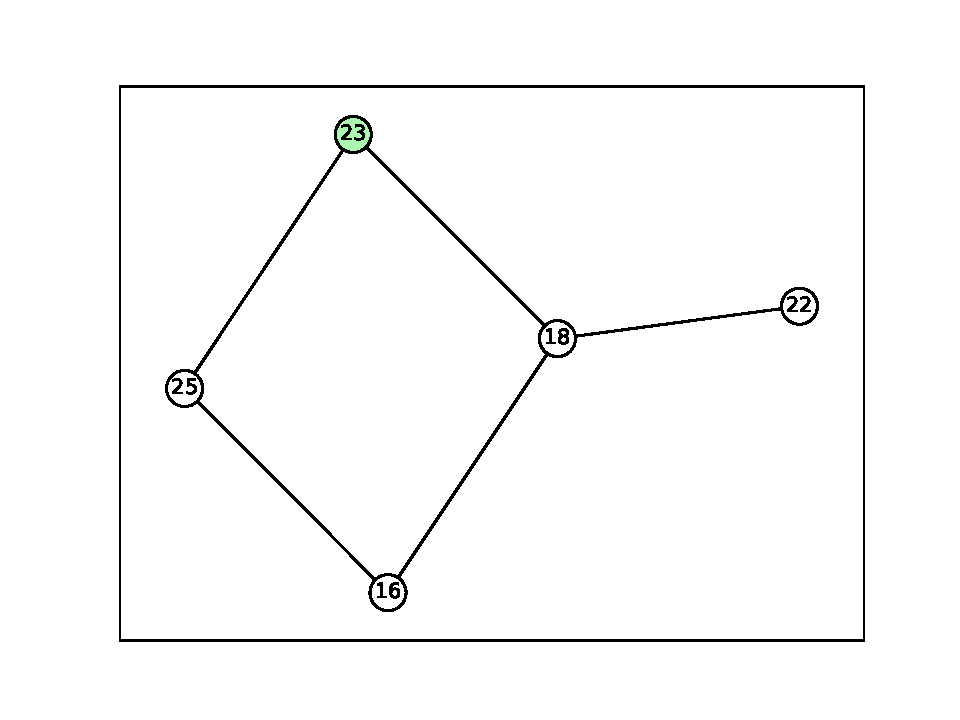
\includegraphics[width=0.5\textwidth]{task11-graphlets/5_16-18-25-22-23.pdf} \\
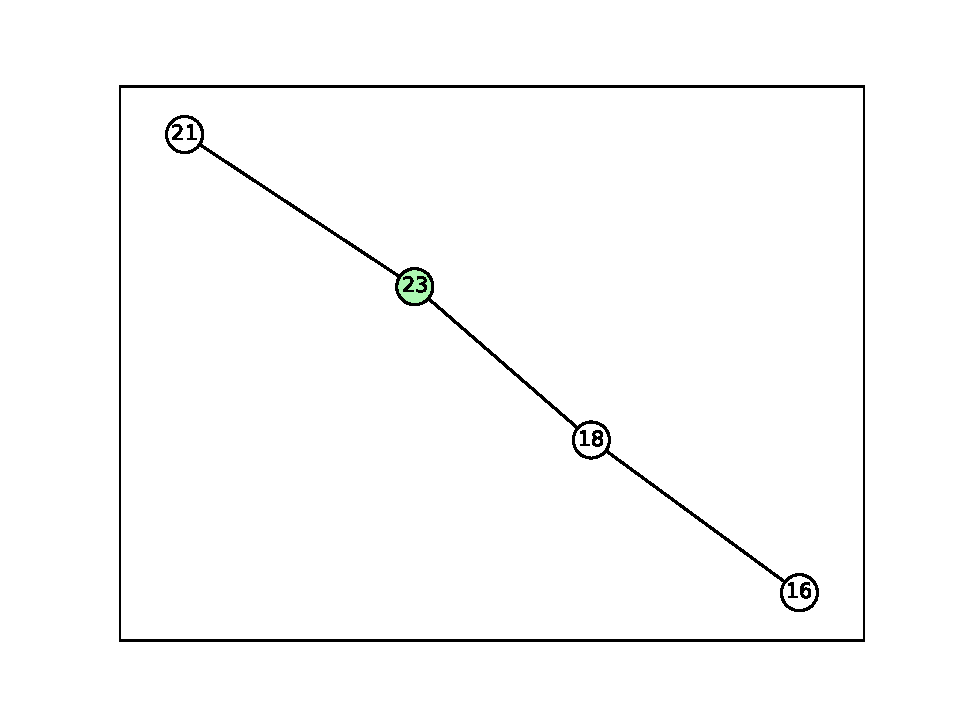
\includegraphics[width=0.5\textwidth]{task11-graphlets/4_16-21-18-23.pdf} &
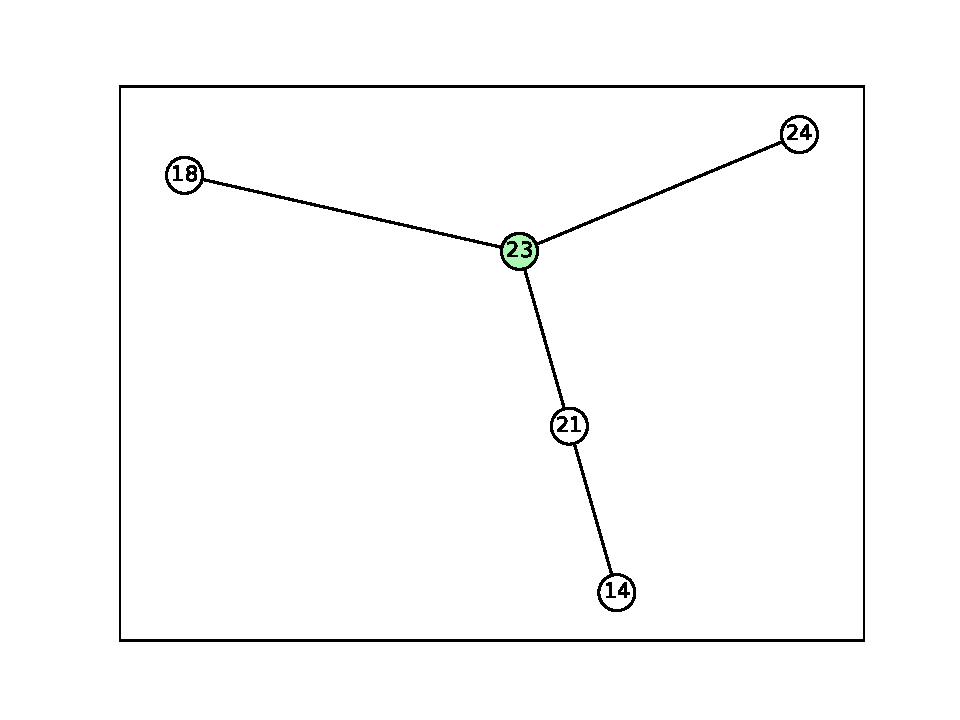
\includegraphics[width=0.5\textwidth]{task11-graphlets/5_14-21-18-23-24.pdf} \\
\end{tabularx}\end{figure}
\begin{figure}\centering\begin{tabularx}{\textwidth}{cc}
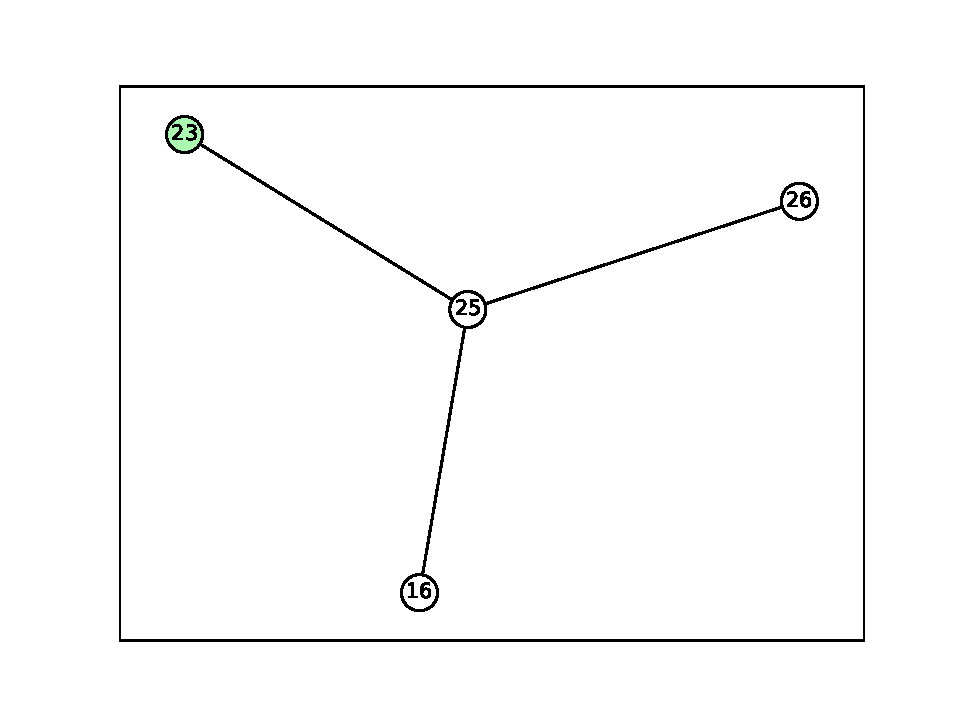
\includegraphics[width=0.5\textwidth]{task11-graphlets/4_16-25-23-26.pdf} &
\includegraphics[width=0.5\textwidth]{task11-graphlets/3_22-23-24.pdf} \\
\includegraphics[width=0.5\textwidth]{task11-graphlets/5_11-14-13-21-23.pdf} &
\includegraphics[width=0.5\textwidth]{task11-graphlets/4_16-17-25-23.pdf} \\
\includegraphics[width=0.5\textwidth]{task11-graphlets/5_21-18-20-22-23.pdf} &
\includegraphics[width=0.5\textwidth]{task11-graphlets/5_16-25-23-24-26.pdf} \\
\includegraphics[width=0.5\textwidth]{task11-graphlets/5_16-18-19-23-24.pdf} &
\includegraphics[width=0.5\textwidth]{task11-graphlets/5_10-11-16-25-23.pdf} \\
\end{tabularx}\end{figure}
\begin{figure}\centering\begin{tabularx}{\textwidth}{cc}
\includegraphics[width=0.5\textwidth]{task11-graphlets/5_14-13-21-20-23.pdf} &
\includegraphics[width=0.5\textwidth]{task11-graphlets/5_14-16-18-19-23.pdf} \\
\includegraphics[width=0.5\textwidth]{task11-graphlets/5_10-16-18-22-23.pdf} &
\includegraphics[width=0.5\textwidth]{task11-graphlets/5_14-16-17-18-23.pdf} \\
\includegraphics[width=0.5\textwidth]{task11-graphlets/4_25-23-24-26.pdf} &
\includegraphics[width=0.5\textwidth]{task11-graphlets/4_18-19-23-24.pdf} \\
\includegraphics[width=0.5\textwidth]{task11-graphlets/5_14-16-13-21-23.pdf} &
\includegraphics[width=0.5\textwidth]{task11-graphlets/4_18-25-22-23.pdf} \\
\end{tabularx}\end{figure}
\begin{figure}\centering\begin{tabularx}{\textwidth}{cc}
\includegraphics[width=0.5\textwidth]{task11-graphlets/4_16-25-23-24.pdf} &
\includegraphics[width=0.5\textwidth]{task11-graphlets/5_21-19-22-23-24.pdf} \\
\includegraphics[width=0.5\textwidth]{task11-graphlets/5_14-16-21-25-23.pdf} &
\includegraphics[width=0.5\textwidth]{task11-graphlets/2_25-23.pdf} \\
\includegraphics[width=0.5\textwidth]{task11-graphlets/5_21-25-19-22-23.pdf} &
\includegraphics[width=0.5\textwidth]{task11-graphlets/5_14-21-17-20-23.pdf} \\
\includegraphics[width=0.5\textwidth]{task11-graphlets/5_10-14-21-23-24.pdf} &
\includegraphics[width=0.5\textwidth]{task11-graphlets/5_14-21-20-23-24.pdf} \\
\end{tabularx}\end{figure}
\begin{figure}\centering\begin{tabularx}{\textwidth}{cc}
\includegraphics[width=0.5\textwidth]{task11-graphlets/5_21-17-20-23-24.pdf} &
\includegraphics[width=0.5\textwidth]{task11-graphlets/5_16-21-17-25-23.pdf} \\
\includegraphics[width=0.5\textwidth]{task11-graphlets/5_14-21-18-19-23.pdf} &
\includegraphics[width=0.5\textwidth]{task11-graphlets/4_14-13-21-23.pdf} \\
\includegraphics[width=0.5\textwidth]{task11-graphlets/3_18-22-23.pdf} &
\includegraphics[width=0.5\textwidth]{task11-graphlets/5_10-14-16-18-23.pdf} \\
\includegraphics[width=0.5\textwidth]{task11-graphlets/4_21-19-22-23.pdf} &
\includegraphics[width=0.5\textwidth]{task11-graphlets/5_18-25-19-23-26.pdf} \\
\end{tabularx}\end{figure}
\begin{figure}\centering\begin{tabularx}{\textwidth}{cc}
\includegraphics[width=0.5\textwidth]{task11-graphlets/4_21-25-23-24.pdf} &
\includegraphics[width=0.5\textwidth]{task11-graphlets/4_14-21-25-23.pdf} \\
\includegraphics[width=0.5\textwidth]{task11-graphlets/5_16-17-25-23-24.pdf} &
\includegraphics[width=0.5\textwidth]{task11-graphlets/5_10-8-16-25-23.pdf} \\
\includegraphics[width=0.5\textwidth]{task11-graphlets/5_16-21-25-23-26.pdf} &
\includegraphics[width=0.5\textwidth]{task11-graphlets/5_16-21-25-23-24.pdf} \\
\includegraphics[width=0.5\textwidth]{task11-graphlets/5_14-13-21-18-23.pdf} &
\includegraphics[width=0.5\textwidth]{task11-graphlets/5_14-16-18-23-24.pdf} \\
\end{tabularx}\end{figure}
\begin{figure}\centering\begin{tabularx}{\textwidth}{cc}
\includegraphics[width=0.5\textwidth]{task11-graphlets/5_16-17-25-23-26.pdf} &
\includegraphics[width=0.5\textwidth]{task11-graphlets/5_21-18-22-23-24.pdf} \\
\includegraphics[width=0.5\textwidth]{task11-graphlets/4_21-25-23-26.pdf} &
\includegraphics[width=0.5\textwidth]{task11-graphlets/5_18-25-19-23-24.pdf} \\
\includegraphics[width=0.5\textwidth]{task11-graphlets/5_14-13-21-22-23.pdf} &
\includegraphics[width=0.5\textwidth]{task11-graphlets/3_16-25-23.pdf} \\
\includegraphics[width=0.5\textwidth]{task11-graphlets/4_16-18-19-23.pdf} &
\includegraphics[width=0.5\textwidth]{task11-graphlets/4_18-22-23-24.pdf} \\
\end{tabularx}\end{figure}
\begin{figure}\centering\begin{tabularx}{\textwidth}{cc}
\includegraphics[width=0.5\textwidth]{task11-graphlets/4_16-17-18-23.pdf} &
\includegraphics[width=0.5\textwidth]{task11-graphlets/5_10-11-16-18-23.pdf} \\
\includegraphics[width=0.5\textwidth]{task11-graphlets/4_14-16-21-23.pdf} &
\includegraphics[width=0.5\textwidth]{task11-graphlets/5_10-8-14-21-23.pdf} \\
\includegraphics[width=0.5\textwidth]{task11-graphlets/5_14-16-25-23-24.pdf} &
\includegraphics[width=0.5\textwidth]{task11-graphlets/3_21-23-24.pdf} \\
\includegraphics[width=0.5\textwidth]{task11-graphlets/5_16-21-18-23-24.pdf} &
\includegraphics[width=0.5\textwidth]{task11-graphlets/4_16-21-25-23.pdf} \\
\end{tabularx}\end{figure}
\begin{figure}\centering\begin{tabularx}{\textwidth}{cc}
\includegraphics[width=0.5\textwidth]{task11-graphlets/4_21-17-20-23.pdf} &
\includegraphics[width=0.5\textwidth]{task11-graphlets/4_21-20-23-24.pdf} \\
\includegraphics[width=0.5\textwidth]{task11-graphlets/5_10-16-18-25-23.pdf} &
\includegraphics[width=0.5\textwidth]{task11-graphlets/2_18-23.pdf} \\
\includegraphics[width=0.5\textwidth]{task11-graphlets/5_14-16-21-18-23.pdf} &
\includegraphics[width=0.5\textwidth]{task11-graphlets/4_21-18-23-24.pdf} \\
\includegraphics[width=0.5\textwidth]{task11-graphlets/5_16-17-18-23-24.pdf} &
\includegraphics[width=0.5\textwidth]{task11-graphlets/5_16-21-17-20-23.pdf} \\
\end{tabularx}\end{figure}
\begin{figure}\centering\begin{tabularx}{\textwidth}{cc}
\includegraphics[width=0.5\textwidth]{task11-graphlets/5_14-16-25-23-26.pdf} &
\includegraphics[width=0.5\textwidth]{task11-graphlets/5_14-16-17-25-23.pdf} \\
\includegraphics[width=0.5\textwidth]{task11-graphlets/3_14-21-23.pdf} &
\includegraphics[width=0.5\textwidth]{task11-graphlets/5_14-13-15-21-23.pdf} \\
\includegraphics[width=0.5\textwidth]{task11-graphlets/5_21-18-25-20-23.pdf} &
\includegraphics[width=0.5\textwidth]{task11-graphlets/5_16-18-22-23-24.pdf} \\
\includegraphics[width=0.5\textwidth]{task11-graphlets/5_14-16-21-22-23.pdf} &
\includegraphics[width=0.5\textwidth]{task11-graphlets/4_14-21-20-23.pdf} \\
\end{tabularx}\end{figure}
\begin{figure}\centering\begin{tabularx}{\textwidth}{cc}
\includegraphics[width=0.5\textwidth]{task11-graphlets/5_21-18-19-23-24.pdf} &
\includegraphics[width=0.5\textwidth]{task11-graphlets/3_18-25-23.pdf} \\
\includegraphics[width=0.5\textwidth]{task11-graphlets/4_14-21-18-23.pdf} &
\includegraphics[width=0.5\textwidth]{task11-graphlets/4_16-18-23-24.pdf} \\
\includegraphics[width=0.5\textwidth]{task11-graphlets/5_21-25-23-24-26.pdf} &
\includegraphics[width=0.5\textwidth]{task11-graphlets/5_14-21-25-23-26.pdf} \\
\includegraphics[width=0.5\textwidth]{task11-graphlets/5_10-8-16-18-23.pdf} &
\includegraphics[width=0.5\textwidth]{task11-graphlets/5_14-16-21-20-23.pdf} \\
\end{tabularx}\end{figure}
\begin{figure}\centering\begin{tabularx}{\textwidth}{cc}
\includegraphics[width=0.5\textwidth]{task11-graphlets/5_10-11-14-21-23.pdf} &
\includegraphics[width=0.5\textwidth]{task11-graphlets/4_14-21-22-23.pdf} \\
\includegraphics[width=0.5\textwidth]{task11-graphlets/4_19-22-23-24.pdf} &
\includegraphics[width=0.5\textwidth]{task11-graphlets/5_10-14-16-25-23.pdf} \\
\includegraphics[width=0.5\textwidth]{task11-graphlets/5_16-21-18-19-23.pdf} &
\includegraphics[width=0.5\textwidth]{task11-graphlets/5_16-21-17-18-23.pdf} \\
\includegraphics[width=0.5\textwidth]{task11-graphlets/5_21-25-20-23-26.pdf} &
\includegraphics[width=0.5\textwidth]{task11-graphlets/5_21-18-25-22-23.pdf} \\
\end{tabularx}\end{figure}
\begin{figure}\centering\begin{tabularx}{\textwidth}{cc}
\includegraphics[width=0.5\textwidth]{task11-graphlets/5_18-25-22-23-24.pdf} &
\includegraphics[width=0.5\textwidth]{task11-graphlets/4_21-18-19-23.pdf} \\
\includegraphics[width=0.5\textwidth]{task11-graphlets/5_18-25-22-23-26.pdf} &
\includegraphics[width=0.5\textwidth]{task11-graphlets/5_16-17-18-19-23.pdf} \\
\includegraphics[width=0.5\textwidth]{task11-graphlets/5_21-25-20-23-24.pdf} &
\includegraphics[width=0.5\textwidth]{task11-graphlets/5_14-21-19-22-23.pdf} \\
\includegraphics[width=0.5\textwidth]{task11-graphlets/3_16-18-23.pdf} &
\includegraphics[width=0.5\textwidth]{task11-graphlets/5_14-21-25-23-24.pdf} \\
\end{tabularx}\end{figure}
\begin{figure}\centering\begin{tabularx}{\textwidth}{cc}
\includegraphics[width=0.5\textwidth]{task11-graphlets/5_14-13-21-25-23.pdf} &
\includegraphics[width=0.5\textwidth]{task11-graphlets/5_21-20-19-22-23.pdf} \\
\includegraphics[width=0.5\textwidth]{task11-graphlets/5_14-16-18-22-23.pdf} &
\includegraphics[width=0.5\textwidth]{task11-graphlets/5_10-16-17-18-23.pdf} \\
\includegraphics[width=0.5\textwidth]{task11-graphlets/4_10-14-21-23.pdf} &
\includegraphics[width=0.5\textwidth]{task11-graphlets/5_10-16-18-19-23.pdf} \\
\includegraphics[width=0.5\textwidth]{task11-graphlets/5_10-14-16-21-23.pdf} &
\includegraphics[width=0.5\textwidth]{task11-graphlets/5_16-21-25-22-23.pdf} \\
\end{tabularx}\end{figure}
\begin{figure}\centering\begin{tabularx}{\textwidth}{cc}
\includegraphics[width=0.5\textwidth]{task11-graphlets/5_14-21-18-20-23.pdf} &
\includegraphics[width=0.5\textwidth]{task11-graphlets/4_25-22-23-24.pdf} \\
\includegraphics[width=0.5\textwidth]{task11-graphlets/4_18-25-19-23.pdf} &
\includegraphics[width=0.5\textwidth]{task11-graphlets/5_10-16-21-25-23.pdf} \\
\includegraphics[width=0.5\textwidth]{task11-graphlets/5_18-25-19-22-23.pdf} &
\includegraphics[width=0.5\textwidth]{task11-graphlets/5_25-19-22-23-24.pdf} \\
\includegraphics[width=0.5\textwidth]{task11-graphlets/5_18-19-22-23-24.pdf} &
\includegraphics[width=0.5\textwidth]{task11-graphlets/5_14-13-21-23-24.pdf} \\
\end{tabularx}\end{figure}
\begin{figure}\centering\begin{tabularx}{\textwidth}{cc}
\includegraphics[width=0.5\textwidth]{task11-graphlets/4_16-18-25-23.pdf} &
\includegraphics[width=0.5\textwidth]{task11-graphlets/5_16-18-25-19-23.pdf} \\
\includegraphics[width=0.5\textwidth]{task11-graphlets/5_16-25-22-23-24.pdf} &
\includegraphics[width=0.5\textwidth]{task11-graphlets/5_21-17-20-22-23.pdf} \\
\includegraphics[width=0.5\textwidth]{task11-graphlets/3_18-23-24.pdf} &
\includegraphics[width=0.5\textwidth]{task11-graphlets/5_14-21-22-23-24.pdf} \\
\includegraphics[width=0.5\textwidth]{task11-graphlets/5_21-20-22-23-24.pdf} &
\includegraphics[width=0.5\textwidth]{task11-graphlets/5_21-18-20-19-23.pdf} \\
\end{tabularx}\end{figure}
\begin{figure}\centering\begin{tabularx}{\textwidth}{cc}
\includegraphics[width=0.5\textwidth]{task11-graphlets/4_21-25-22-23.pdf} &
\includegraphics[width=0.5\textwidth]{task11-graphlets/5_10-14-21-20-23.pdf} \\
\includegraphics[width=0.5\textwidth]{task11-graphlets/4_21-18-25-23.pdf} &
\includegraphics[width=0.5\textwidth]{task11-graphlets/5_10-14-21-18-23.pdf} \\
\includegraphics[width=0.5\textwidth]{task11-graphlets/4_18-19-22-23.pdf} &
\includegraphics[width=0.5\textwidth]{task11-graphlets/5_16-17-18-25-23.pdf} \\
\includegraphics[width=0.5\textwidth]{task11-graphlets/5_10-16-18-23-24.pdf} &
\includegraphics[width=0.5\textwidth]{task11-graphlets/5_16-17-25-20-23.pdf} \\
\end{tabularx}\end{figure}
\begin{figure}\centering\begin{tabularx}{\textwidth}{cc}
\includegraphics[width=0.5\textwidth]{task11-graphlets/5_16-18-25-23-26.pdf} &
\includegraphics[width=0.5\textwidth]{task11-graphlets/5_12-14-13-21-23.pdf} \\
\includegraphics[width=0.5\textwidth]{task11-graphlets/4_21-25-20-23.pdf} &
\includegraphics[width=0.5\textwidth]{task11-graphlets/4_14-16-25-23.pdf} \\
\includegraphics[width=0.5\textwidth]{task11-graphlets/5_14-21-20-22-23.pdf} &
\includegraphics[width=0.5\textwidth]{task11-graphlets/5_10-14-21-22-23.pdf} \\
\includegraphics[width=0.5\textwidth]{task11-graphlets/4_18-25-23-24.pdf} &
\includegraphics[width=0.5\textwidth]{task11-graphlets/4_10-16-18-23.pdf} \\
\end{tabularx}\end{figure}
\begin{figure}\centering\begin{tabularx}{\textwidth}{cc}
\includegraphics[width=0.5\textwidth]{task11-graphlets/3_18-19-23.pdf} &
\includegraphics[width=0.5\textwidth]{task11-graphlets/5_14-16-13-18-23.pdf} \\
\includegraphics[width=0.5\textwidth]{task11-graphlets/5_14-21-18-22-23.pdf} &
\includegraphics[width=0.5\textwidth]{task11-graphlets/5_16-21-25-20-23.pdf} \\
\includegraphics[width=0.5\textwidth]{task11-graphlets/4_18-25-23-26.pdf} &
\includegraphics[width=0.5\textwidth]{task11-graphlets/5_16-18-25-23-24.pdf} \\
\includegraphics[width=0.5\textwidth]{task11-graphlets/5_5-10-16-25-23.pdf} &
\includegraphics[width=0.5\textwidth]{task11-graphlets/5_16-21-18-25-23.pdf} \\
\end{tabularx}\end{figure}
\begin{figure}\centering\begin{tabularx}{\textwidth}{cc}
\includegraphics[width=0.5\textwidth]{task11-graphlets/5_21-17-18-20-23.pdf} &
\includegraphics[width=0.5\textwidth]{task11-graphlets/5_16-18-19-22-23.pdf} \\
\includegraphics[width=0.5\textwidth]{task11-graphlets/5_21-18-20-23-24.pdf} &
\includegraphics[width=0.5\textwidth]{task11-graphlets/3_21-25-23.pdf} \\
\multicolumn{2}{c}{
\includegraphics[width=0.5\textwidth]{task11-graphlets/5_21-25-20-22-23.pdf}}
\end{tabularx}\end{figure}
\end{document}
